
% Copyright (c)  2007-2012  Tim Niemueller, RWTH Aachen University
%
% Created: Mon Aug 13 16:55:22 2012

%aspectratio=169
\documentclass[compress,xcolor=table,nominiframes,notitlehead,noframetitlebg,addurl]{beamer}
% add handout to optional args for handout version

%\usepackage{hyperref}
\usepackage{beamerthemesplit}
\usepackage[utf8]{inputenc}
\usepackage[T1]{fontenc}
\usepackage[german]{babel}
\usepackage{german}
\usepackage{graphicx}
\usepackage{subfigure}
\usepackage{epsfig}
\usepackage{tabularx}
\usepackage{latexsym}
\usepackage{url}
\usepackage{tikz}
\usepackage{multimedia}
\usepackage{xcolor}
\usepackage{listings}
\usepackage{verbatim}
\usepackage{colortbl}
\usepackage{psfrag}
\usepackage{xifthen}
\usepackage[absolute,overlay]{textpos}
\usepackage{palatino}
\usepackage{enumitem}

\graphicspath{{../},{./images/},{./images/},{./figures/}}

%% Mulberry Color for highlighting
\definecolor{Mulberry}{cmyk}{0.34,0.90,0,0.02}
\definecolor{Lavender}{cmyk}{0,0.48,0,0}
\definecolor{Melon}{cmyk}{0,0.46,0.50,0}
\definecolor{Peach}{cmyk}{0,0.50,0.70,0}
\definecolor{RedOrange}{cmyk}{0,0.77,0.87,0}
\definecolor{BrickRed}{cmyk}{0,0.89,0.94,0.28}
\definecolor{Mahogany}{cmyk}{0,0.85,0.87,0.35}
\definecolor{BurntOrange}{cmyk}{0,0.51,1,0}
\definecolor{BitterSweet}{cmyk}{0,0.75,1,0.24}
\definecolor{RosBlue}{rgb}{0.19,0.25,0.38}


\mode<presentation>
{
  \usetheme{FawkesMinimal}

  % to hide nav bar uncomment this line
  \setbeamertemplate{navigation symbols}{}

  %\setbeamercovered{transparent}
  \setbeamercovered{%
    invisible,
    again covered={\opaqueness<1->{40}}
  }

  \setbeamerfont{author}{size=\footnotesize,family=\rmfamily,parent=structure}
}

% Usage notes for handout version:
% Compile the beamer version immediately before you build the handout version,
% otherwise page numbers etc. will be wrong! The .aux files are *not* updated
% in handout mode, see PGF Manual for details why this is necessary.
% Comment out below one of the two pgfuselayout lines for either 2 or 4 slides
% per page. To have a very light grey background uncomment the background canvas
% color line. The logical page options are used to draw borders around each
% slide.
\mode<handout>
{
  \usetheme{Fawkes}

  % to hide nav bar uncomment this line
  \setbeamertemplate{navigation symbols}{}

  %\setbeamercovered{transparent}
  \setbeamercovered{%
    again covered={\opaqueness<1->{40}}
  }

  % Very slight grey background, can be used instead of borders
  %\setbeamercolor{background canvas}{bg=black!5}

  \usepackage{pgfpages}
  \pgfpagesuselayout{4 on 1}[a4paper,border shrink=5mm,landscape]
  %\pgfpagesuselayout{2 on 1}[a4paper,border shrink=5mm]

  \pgfpageslogicalpageoptions{1}{border code=\pgfstroke}
  \pgfpageslogicalpageoptions{2}{border code=\pgfstroke}
  \pgfpageslogicalpageoptions{3}{border code=\pgfstroke}
  \pgfpageslogicalpageoptions{4}{border code=\pgfstroke}
  \nofiles
}


% Declare layers
\pgfdeclarelayer{background}
\pgfsetlayers{background,main} 

% Load PGF libraries
\usetikzlibrary{patterns}
\usetikzlibrary{arrows}
\usetikzlibrary{topaths}
\usetikzlibrary{snakes}
\usetikzlibrary{calc}
\usetikzlibrary{positioning}
\usetikzlibrary{shadows}
\usetikzlibrary{shapes.multipart}
\usetikzlibrary{arrows.meta}
\usetikzlibrary{fit,arrows,decorations.pathreplacing,decorations.text}


% set lengths for textpos package
\setlength{\TPHorizModule}{10mm}
\setlength{\TPVertModule}{\TPHorizModule}
\textblockorigin{8mm}{16mm} % start everything near the top-left corner
\setbeamercolor{textblock color}{fg=blue!50,bg=white}

\institute{%
  %\vspace{1cm}
  \begin{minipage}{\textwidth}\centering
  
\includegraphics[height=0.6cm]{common/images/logos/rwth-logo}
  \quad\quad
  
\includegraphics[height=0.6cm]{common/images/logos/kbsg}
  \end{minipage}
}

\setlist[itemize]{leftmargin=12pt,label=\usebeamerfont*{itemize item}%
  \usebeamercolor[fg]{itemize item}
  \usebeamertemplate{itemize item}}
\setlist[description]{leftmargin=4pt,itemindent=0pt,font=\color{FawkesOrange}}
\setenumerate[1]{%
  leftmargin=12pt,%
  label=\protect\usebeamerfont{enumerate item}%
        \protect\usebeamercolor[fg]{enumerate item}%
        \insertenumlabel.}

%numbers=left, numberstyle=\tiny, stepnumber=2, numbersep=5pt
\lstset{language=[GNU]C++,
        basicstyle=\small,
        escapeinside={/*(*/}{/*)*/},
        breaklines=true,
        showstringspaces=false
        }

% Uncomment the listings styles you need
\lstdefinelanguage{Lua}
{
  morekeywords={and,break,do,else,elseif,end,false,for,function,
                if,in,local,nil,not,or,repeat,return,then,true,until,while},
  sensitive=true,
  morecomment=[l]{--},
  morecomment=[s]{--[[}{--]]},
  morestring=[b]{"},
  morestring=[s]{[==[}{]==]},
}

% default style
\lstdefinestyle{Lua}
{
  language=Lua,
  basicstyle=\ttfamily,
  breaklines=true,
  showstringspaces=false,
  %keywordstyle=\bfseries,
  keywordstyle=\color{Mulberry},
  %frame=lines,
  %belowcaptionskip=8pt,
  emphstyle=\itshape,
  %numbers=left,
  stepnumber=1,
  %backgroundcolor=\color{blue!10},
  rulecolor=\color{blue!50},
  fillcolor=\color{blue!20},
  %framexleftmargin=18pt,
  %xleftmargin=18pt,
  stringstyle=\color{BitterSweet},
  %stringstyle=\color{BrickRed},
  commentstyle=\color{BrickRed},
  escapechar=\%
  % emph={getup, servo, depends_skills},
  %emphstyle=\underbar,
  %numbers=left,
  %stepnumber=1,
  %%stringstyle=\ttfamily, % typewriter type for strings
}
\lstdefinestyle{SmallLua}{
  style=Lua,
  basicstyle=\ttfamily\footnotesize,
  numbersep=6pt,
}
\lstdefinestyle{ReallySmallLua}{
  style=Lua,
  basicstyle=\ttfamily\tiny,
  numbersep=5pt,
}

\lstdefinelanguage{Yaml}
{
  keywords={true,false,null,y,n},
  sensitive=false,
  comment=[l]{\#},
  morecomment=[s]{/*}{*/},
  morestring=[b]',
  morestring=[b]",
}

% default style
\lstdefinestyle{Yaml}
{
  language=Yaml,
  basicstyle=\YAMLkeystyle,
  breaklines=true,
  showstringspaces=false,
  %keywordstyle=\bfseries,
  keywordstyle=\color{Mulberry},
  %frame=lines,
  %belowcaptionskip=8pt,
  emphstyle=\itshape,
  %numbers=left,
  stepnumber=1,
  %backgroundcolor=\color{blue!10},
  rulecolor=\color{blue!50},
  fillcolor=\color{blue!20},
  %framexleftmargin=18pt,
  %xleftmargin=18pt,
  stringstyle=\color{BitterSweet},
  %stringstyle=\color{BrickRed},
  commentstyle=\color{BrickRed},
  escapechar=\%
  % emph={getup, servo, depends_skills},
  %emphstyle=\underbar,
  %numbers=left,
  %stepnumber=1,
  %%stringstyle=\ttfamily, % typewriter type for strings
}
\lstdefinestyle{SmallYaml}{
  style=Yaml,
  basicstyle=\ttfamily\footnotesize,
  numbersep=6pt,
}
\lstdefinestyle{ReallySmallYaml}{
  style=Yaml,
  basicstyle=\ttfamily\tiny,
  numbersep=5pt,
}

%\lstdefinelanguage{OpenPRS}{
  keywordsprefix=\$,
  %keywordsprefix=\$,
  alsoletter={?!=-<>*\$^~},
  keywordstyle=\color{Mulberry!80!black}\bfseries,
  keywords=[2]{:invocation, :context, :call, :body, :action,
    :setting, :documentation, :effects, defop},
  keywordstyle=[2]\color{BrickRed!70!blue}\bfseries,
  keywords=[3]{?, !, ^, ~, =>, ~>, =, if, else, elseif, do, while, //},
  keywordstyle=[3]\color{darkgray}\bfseries,
  keywords=[4]{start-critical-section, end-critical-section, equal,
    print, printf},%
  keywordstyle=[4]\color{gray}\bfseries,
  %identifierstyle=\color{black},
  sensitive=false,
  comment=[l]{;},
  commentstyle=\color{purple}\ttfamily,
  stringstyle=\color{red}\ttfamily,
  morestring=[b]"
}


\lstdefinestyle{OpenPRS}
{
  language=OpenPRS,
  basicstyle=\footnotesize\ttfamily\vspace{0.2cm},
  breaklines=true,
  showstringspaces=false,
  %keywordstyle=\bfseries,
  %keywordstyle=\color{Mulberry},
  frame=lines,
  belowcaptionskip=8pt,
  emphstyle=\itshape,
  numbers=left,
  stepnumber=1,
  backgroundcolor=\color{blue!10},
  rulecolor=\color{blue!50},
  fillcolor=\color{blue!20},
  framexleftmargin=16pt,
  xleftmargin=16pt,
  %stringstyle=\color{BitterSweet},
  stringstyle=\color{BrickRed},
  commentstyle=\color{BrickRed},
  escapechar=\%
  % emph={getup, servo, depends_skills},
  %emphstyle=\underbar,
  %numbers=left,
  %stepnumber=1,
  %%stringstyle=\ttfamily, % typewriter type for strings
}

\lstdefinestyle{SmallOpenPRS}{
  style=OpenPRS,
  basicstyle=\ttfamily\footnotesize,
  numbersep=6pt,
}
\lstdefinestyle{ReallySmallOpenPRS}{
  style=OpenPRS,
  basicstyle=\ttfamily\scriptsize,
  numbersep=5pt,
}

\lstdefinestyle{ReallySmallOpenPRSNoFrame}{
  style=OpenPRS,
  basicstyle=\ttfamily\scriptsize,
  numbersep=5pt,
  frame=none,
  backgroundcolor=\color{white},
  framextopmargin=0pt,
  framexbottommargin=0pt
}

\lstdefinestyle{SuperSmallOpenPRSNoFrame}{
  style=OpenPRS,
  basicstyle=\ttfamily\fontsize{10pt}{10pt}\selectfont,
  numbers=none,
  frame=none,
  backgroundcolor=\color{white},
  framextopmargin=0pt,
  framexbottommargin=0pt,
  framexleftmargin=-2pt, xleftmargin=-2pt,
}

\lstdefinestyle{SmallOpenPRSNoFrame}{
  style=OpenPRS,
  basicstyle=\ttfamily\footnotesize,
  numbersep=5pt,
  frame=none,
  backgroundcolor=\color{white},
  framextopmargin=0pt,
  framexbottommargin=0pt
}

\lstdefinelanguage{CLIPS}{
  keywordsprefix=?,
  %keywordsprefix=\$,
  alsoletter={?=-<>*\$},
  keywordstyle=\color{Mulberry!80!black}\bfseries,
  keywords=[2]{deffunction, deftemplate, defrule, deffacts, defgeneric,
    defmodule, defadvice, defglobal, defmethod, definstance, defclass},
  keywordstyle=[2]\color{BrickRed!70!blue}\bfseries,
  keywords=[3]{slot, multislot, type, default, default-dynamic,
                      extends, crlf, range, nil, if, then, else, while,
                      not, or, switch, case, and, reset,
                      assert, test, declare, salience, return, bind, modify,
                      retract, explicit, unique, node-index-hash,
                      halt, printout, =>, <-},
  keywordstyle=[3]\color{darkgray}\bfseries,
  keywords=[4]{subsetp,progn, progn$, not, node-index-hash, create$,
    append$, length$, printout},%
  keywordstyle=[4]\color{gray}\bfseries,
  %identifierstyle=\color{black},
  sensitive=false,
  comment=[l]{;},
  commentstyle=\color{purple}\ttfamily,
  stringstyle=\color{red}\ttfamily,
  morestring=[b]"
}


\lstdefinestyle{CLIPS}
{
  language=CLIPS,
  basicstyle=\footnotesize\ttfamily\vspace{0.2cm},
  breaklines=true,
  showstringspaces=false,
  %keywordstyle=\bfseries,
  %keywordstyle=\color{Mulberry},
  frame=lines,
  belowcaptionskip=-3pt,
  emphstyle=\itshape,
  numbers=left,
  stepnumber=1,
  backgroundcolor=\color{gray!10},
  rulecolor=\color{gray!80},
  fillcolor=\color{gray!10},
  framexleftmargin=16pt,
  xleftmargin=16pt,
  %stringstyle=\color{BitterSweet},
  stringstyle=\color{BrickRed},
  commentstyle=\color{BrickRed},
  escapechar=\%,
  % emph={getup, servo, depends_skills},
  %emphstyle=\underbar,
  %numbers=left,
  %stepnumber=1,
  %%stringstyle=\ttfamily, % typewriter type for strings
  %float,
  captionpos=b
}

\lstdefinestyle{SmallCLIPS}{
  style=CLIPS,
  basicstyle=\ttfamily\footnotesize,
  numbersep=6pt,
}
\lstdefinestyle{ReallySmallCLIPS}{
  style=CLIPS,
  basicstyle=\ttfamily\scriptsize,
  numbersep=5pt,
}

\lstdefinestyle{ReallySmallCLIPSNoFrame}{
  style=CLIPS,
  basicstyle=\ttfamily\scriptsize,
  numbersep=5pt,
  frame=none,
  backgroundcolor=\color{white},
  framextopmargin=0pt,
  framexbottommargin=0pt
}

\lstdefinestyle{SuperSmallCLIPSNoFrame}{
  style=CLIPS,
  basicstyle=\ttfamily\fontsize{10pt}{10pt}\selectfont,
  numbers=none,
  frame=none,
  backgroundcolor=\color{white},
  framextopmargin=0pt,
  framexbottommargin=0pt,
  framexleftmargin=-2pt, xleftmargin=-2pt,
}

\lstdefinestyle{SmallCLIPSNoFrame}{
  style=CLIPS,
  basicstyle=\ttfamily\footnotesize,
  numbersep=5pt,
  frame=none,
  backgroundcolor=\color{white},
  framextopmargin=0pt,
  framexbottommargin=0pt
}

%\lstdefinelanguage{JavaScript}{
  keywords={typeof, new, true, false, catch, function, return, null, catch, switch, var, if, in, while, do, else, case, break},
  keywordstyle=\color{blue}\bfseries,
  ndkeywords={class, export, boolean, throw, implements, import}, %, this
  ndkeywordstyle=\color{darkgray}\bfseries,
  identifierstyle=\color{black},
  sensitive=false,
  comment=[l]{//},
  morecomment=[s]{/*}{*/},
  commentstyle=\color{purple}\ttfamily,
  stringstyle=\color{red}\ttfamily,
  morestring=[b]',
  morestring=[b]"
}

\lstdefinestyle{JSON}
{
  language=JavaScript,
  morekeywords={interface,field,message,comment},
  basicstyle=\footnotesize\ttfamily\vspace{0.2cm},
  breaklines=true,
  showstringspaces=false,
  %keywordstyle=\bfseries,
  keywordstyle=\color{Mulberry},
  frame=lines,
  belowcaptionskip=8pt,
  emphstyle=\itshape,
  numbers=left,
  stepnumber=1,
  backgroundcolor=\color{blue!10},
  rulecolor=\color{blue!50},
  fillcolor=\color{blue!20},
  framexleftmargin=16pt,
  xleftmargin=16pt,
  %stringstyle=\color{BitterSweet},
  stringstyle=\color{BrickRed},
  commentstyle=\color{BrickRed},
  escapechar=\%,
  % emph={getup, servo, depends_skills},
  %emphstyle=\underbar,
  %numbers=left,
  %stepnumber=1,
  %%stringstyle=\ttfamily, % typewriter type for strings
  captionpos=b
}

\lstdefinestyle{SmallJSON}{
  style=JSON,
  basicstyle=\ttfamily\footnotesize,
  numbersep=6pt,
}
\lstdefinestyle{ReallySmallJSON}{
  style=JSON,
  basicstyle=\ttfamily\tiny,
  numbersep=5pt,
}

\definecolor{dkgreen}{rgb}{0,0.6,0}
\definecolor{gray}{rgb}{0.5,0.5,0.5}
\definecolor{mauve}{rgb}{0.58,0,0.82}
\definecolor{gray}{rgb}{0.4,0.4,0.4}
\definecolor{darkblue}{rgb}{0.0,0.0,0.6}
\definecolor{lightblue}{rgb}{0.0,0.0,0.9}
\definecolor{cyan}{rgb}{0.0,0.6,0.6}
\definecolor{darkred}{rgb}{0.6,0.0,0.0}


\lstdefinelanguage{XML}
{
  basicstyle=\ttfamily\footnotesize,
  columns=fullflexible,
  showstringspaces=false,
  numbers=left,                   % where to put the line-numbers
  numberstyle=\tiny\color{gray},  % the style that is used for the line-numbers
  stepnumber=1,
  numbersep=5pt,                  % how far the line-numbers are from the code
  backgroundcolor=\color{white},      % choose the background color. You must add \usepackage{color}
  showspaces=false,               % show spaces adding particular underscores
  showstringspaces=false,         % underline spaces within strings
  showtabs=false,                 % show tabs within strings adding particular underscores
  frame=none,                   % adds a frame around the code
  rulecolor=\color{black},        % if not set, the frame-color may be changed on line-breaks within not-black text (e.g. commens (green here))
  tabsize=2,                      % sets default tabsize to 2 spaces
  captionpos=b,                   % sets the caption-position to bottom
  breaklines=true,                % sets automatic line breaking
  breakatwhitespace=false,        % sets if automatic breaks should only happen at whitespace
  title=\lstname,                   % show the filename of files included with \lstinputlisting;
                                  % also try caption instead of title  
  commentstyle=\color{gray}\upshape,
  morestring=[s][\color{mauve}]{"}{"},
  morestring=[s][\color{black}]{>}{<},
  morecomment=[s]{<?}{?>},
  morecomment=[s][\color{dkgreen}]{<!--}{-->},
  stringstyle=\color{black},
  identifierstyle=\color{lightblue},
  keywordstyle=\color{red},
  morekeywords={xmlns,xsi,noNamespaceSchemaLocation,type,id,x,y,source,target,version,tool,transRef,roleRef,objective,eventually},
  basicstyle=\ttfamily\scriptsize,
  backgroundcolor=\color{blue!10},
  numbers=none,
  numbersep=5pt
}


% Default style
\lstset{style=Lua}

% Hyphenation of words with hyphen
\def\hyph{-\penalty0\hskip0pt\relax}

% define an anchor in the frame
\newcommand{\tikzref}[1]{%
  \tikz[remember picture]{%
    \coordinate (#1) at (0,0.5ex);%
  }%
}%


%%% Local Variables: 
%%% mode: latex
%%% TeX-master: "aaai-spring2013-clips-agent"
%%% End: 

\lstdefinelanguage{CLIPS}{
  keywordsprefix=?,
  %keywordsprefix=\$,
  alsoletter={?=-<>*\$},
  keywordstyle=\color{Mulberry!80!black}\bfseries,
  keywords=[2]{deffunction, deftemplate, defrule, deffacts, defgeneric,
    defmodule, defadvice, defglobal, defmethod, definstance, defclass},
  keywordstyle=[2]\color{BrickRed!70!blue}\bfseries,
  keywords=[3]{slot, multislot, type, default, default-dynamic,
                      extends, crlf, range, nil, if, then, else, while,
                      not, or, switch, case, and, reset,
                      assert, test, declare, salience, return, bind, modify,
                      retract, explicit, unique, node-index-hash,
                      halt, printout, =>, <-},
  keywordstyle=[3]\color{darkgray}\bfseries,
  keywords=[4]{subsetp,progn, progn$, not, node-index-hash, create$,
    append$, length$, printout},%
  keywordstyle=[4]\color{gray}\bfseries,
  %identifierstyle=\color{black},
  sensitive=false,
  comment=[l]{;},
  commentstyle=\color{purple}\ttfamily,
  stringstyle=\color{red}\ttfamily,
  morestring=[b]"
}


\lstdefinestyle{CLIPS}
{
  language=CLIPS,
  basicstyle=\footnotesize\ttfamily\vspace{0.2cm},
  breaklines=true,
  showstringspaces=false,
  %keywordstyle=\bfseries,
  %keywordstyle=\color{Mulberry},
  frame=lines,
  belowcaptionskip=-3pt,
  emphstyle=\itshape,
  numbers=left,
  stepnumber=1,
  backgroundcolor=\color{gray!10},
  rulecolor=\color{gray!80},
  fillcolor=\color{gray!10},
  framexleftmargin=16pt,
  xleftmargin=16pt,
  %stringstyle=\color{BitterSweet},
  stringstyle=\color{BrickRed},
  commentstyle=\color{BrickRed},
  escapechar=\%,
  % emph={getup, servo, depends_skills},
  %emphstyle=\underbar,
  %numbers=left,
  %stepnumber=1,
  %%stringstyle=\ttfamily, % typewriter type for strings
  %float,
  captionpos=b
}

\lstdefinestyle{SmallCLIPS}{
  style=CLIPS,
  basicstyle=\ttfamily\footnotesize,
  numbersep=6pt,
}
\lstdefinestyle{ReallySmallCLIPS}{
  style=CLIPS,
  basicstyle=\ttfamily\scriptsize,
  numbersep=5pt,
}

\lstdefinestyle{ReallySmallCLIPSNoFrame}{
  style=CLIPS,
  basicstyle=\ttfamily\scriptsize,
  numbersep=5pt,
  frame=none,
  backgroundcolor=\color{white},
  framextopmargin=0pt,
  framexbottommargin=0pt
}

\lstdefinestyle{SuperSmallCLIPSNoFrame}{
  style=CLIPS,
  basicstyle=\ttfamily\fontsize{10pt}{10pt}\selectfont,
  numbers=none,
  frame=none,
  backgroundcolor=\color{white},
  framextopmargin=0pt,
  framexbottommargin=0pt,
  framexleftmargin=-2pt, xleftmargin=-2pt,
}

\lstdefinestyle{SmallCLIPSNoFrame}{
  style=CLIPS,
  basicstyle=\ttfamily\footnotesize,
  numbersep=5pt,
  frame=none,
  backgroundcolor=\color{white},
  framextopmargin=0pt,
  framexbottommargin=0pt
}

\lstdefinelanguage{JavaScript}{
  keywords={typeof, new, true, false, catch, function, return, null, catch, switch, var, if, in, while, do, else, case, break},
  keywordstyle=\color{blue}\bfseries,
  ndkeywords={class, export, boolean, throw, implements, import}, %, this
  ndkeywordstyle=\color{darkgray}\bfseries,
  identifierstyle=\color{black},
  sensitive=false,
  comment=[l]{//},
  morecomment=[s]{/*}{*/},
  commentstyle=\color{purple}\ttfamily,
  stringstyle=\color{red}\ttfamily,
  morestring=[b]',
  morestring=[b]"
}

\lstdefinestyle{JSON}
{
  language=JavaScript,
  morekeywords={interface,field,message,comment},
  basicstyle=\footnotesize\ttfamily\vspace{0.2cm},
  breaklines=true,
  showstringspaces=false,
  %keywordstyle=\bfseries,
  keywordstyle=\color{Mulberry},
  frame=lines,
  belowcaptionskip=8pt,
  emphstyle=\itshape,
  numbers=left,
  stepnumber=1,
  backgroundcolor=\color{blue!10},
  rulecolor=\color{blue!50},
  fillcolor=\color{blue!20},
  framexleftmargin=16pt,
  xleftmargin=16pt,
  %stringstyle=\color{BitterSweet},
  stringstyle=\color{BrickRed},
  commentstyle=\color{BrickRed},
  escapechar=\%,
  % emph={getup, servo, depends_skills},
  %emphstyle=\underbar,
  %numbers=left,
  %stepnumber=1,
  %%stringstyle=\ttfamily, % typewriter type for strings
  captionpos=b
}

\lstdefinestyle{SmallJSON}{
  style=JSON,
  basicstyle=\ttfamily\footnotesize,
  numbersep=6pt,
}
\lstdefinestyle{ReallySmallJSON}{
  style=JSON,
  basicstyle=\ttfamily\tiny,
  numbersep=5pt,
}

\lstdefinelanguage{PDDL}{
  keywordsprefix=:,
  keywords={define, problem},
  keywordstyle=\color{blue}\bfseries,
  ndkeywords={}, %, this
  ndkeywordstyle=\color{darkgray}\bfseries,
  identifierstyle=\color{black},
  sensitive=false,
  comment=[l]{//},
  morecomment=[s]{<<}{>>},
  commentstyle=\color{darkgray}\ttfamily,
  stringstyle=\color{red}\ttfamily,
  morestring=[b]',
  morestring=[b]"
}

\lstdefinestyle{PDDL}
{
  language=PDDL,
  morekeywords={interface,field,message,comment},
  basicstyle=\footnotesize\ttfamily\vspace{0.2cm},
  breaklines=true,
  showstringspaces=false,
  %keywordstyle=\bfseries,
  keywordstyle=\color{Mulberry},
  frame=lines,
  belowcaptionskip=8pt,
  emphstyle=\itshape,
  numbers=left,
  stepnumber=1,
  backgroundcolor=\color{blue!10},
  rulecolor=\color{blue!50},
  fillcolor=\color{blue!20},
  framexleftmargin=16pt,
  xleftmargin=16pt,
  %stringstyle=\color{BitterSweet},
  stringstyle=\color{BrickRed},
  commentstyle=\color{darkgray},
  escapechar=\%,
  % emph={getup, servo, depends_skills},
  %emphstyle=\underbar,
  %numbers=left,
  %stepnumber=1,
  %%stringstyle=\ttfamily, % typewriter type for strings
  captionpos=b
}

\lstdefinestyle{SmallPDDL}{
  style=PDDL,
  basicstyle=\ttfamily\footnotesize,
  numbersep=6pt,
}
\lstdefinestyle{SmallSlidePDDL}{
  style=PDDL,
  basicstyle=\ttfamily\footnotesize,
  numbersep=6pt,
  backgroundcolor=\color{gray!10},
  rulecolor=\color{gray!80},
  fillcolor=\color{gray!10},
}
\lstdefinestyle{ReallySmallPDDL}{
  style=PDDL,
  basicstyle=\ttfamily\tiny,
  numbersep=5pt,
}


\usepackage{todonotes}
\usepackage{booktabs}
\newcommand{\tabitem}{~~\llap{\textcolor{FawkesOrange}{\textbullet}}~~}


\hypersetup{
  pdftitle      = {Robot Memory-Master Thesis Presentation},
  pdfauthor     = {Frederik Zwilling},
  pdfkeywords   = {robotics, artificial intelligence, robot memory, logistics, RCLL, @Home},
  pdfsubject    = {Master Thesis Presentation}
  %hidelinks    = true
}

\title[Robot Memory] {A Document-Oriented Robot Memory\\ for
  Knowledge Sharing and Hybrid Reasoning\\ on Mobile Robots}
\author[Zwilling]{
  \textbf{Frederik Zwilling}\\
  ~Supervisors: Prof. Lakemeyer, PhD., Prof. Dr. Jarke\\
  ~Adviser: Tim Niemueller
}
\def\projecturl{}

\date[Mar 15th 2017]{Mar 15th 2017 -- Master Thesis Presentation}

\begin{document}
\shorthandoff{"} % aus "o kein ö machen

\frame[plain]{\titlepage}
\addtocounter{framenumber}{-1}

\begin{frame}[plain]
  \frametitle{Robot Memory at a Glance}
  \textbf{\large Database to store information of a robot about its environment}
  \bigskip
  \begin{itemize}
  \item \textbf{Domain:} Logistics and domestic service robots
  \item \textbf{Purpose:} Scalable storage and rich querying
  \item \textbf{Focus:} Knowledge sharing and hybrid reasoning\\ for knowledge-based systems
  \end{itemize}
\end{frame}

\addtocounter{framenumber}{-1}

\section{Motivation}
\begin{frame}[plain]
  \tableofcontents[currentsection]
\end{frame}
\addtocounter{framenumber}{-1}

\begin{frame}
  \frametitle{Why do robots need a memory?}
  \vspace{1cm}
  \begin{columns}
    \begin{column}{0.5\textwidth}
    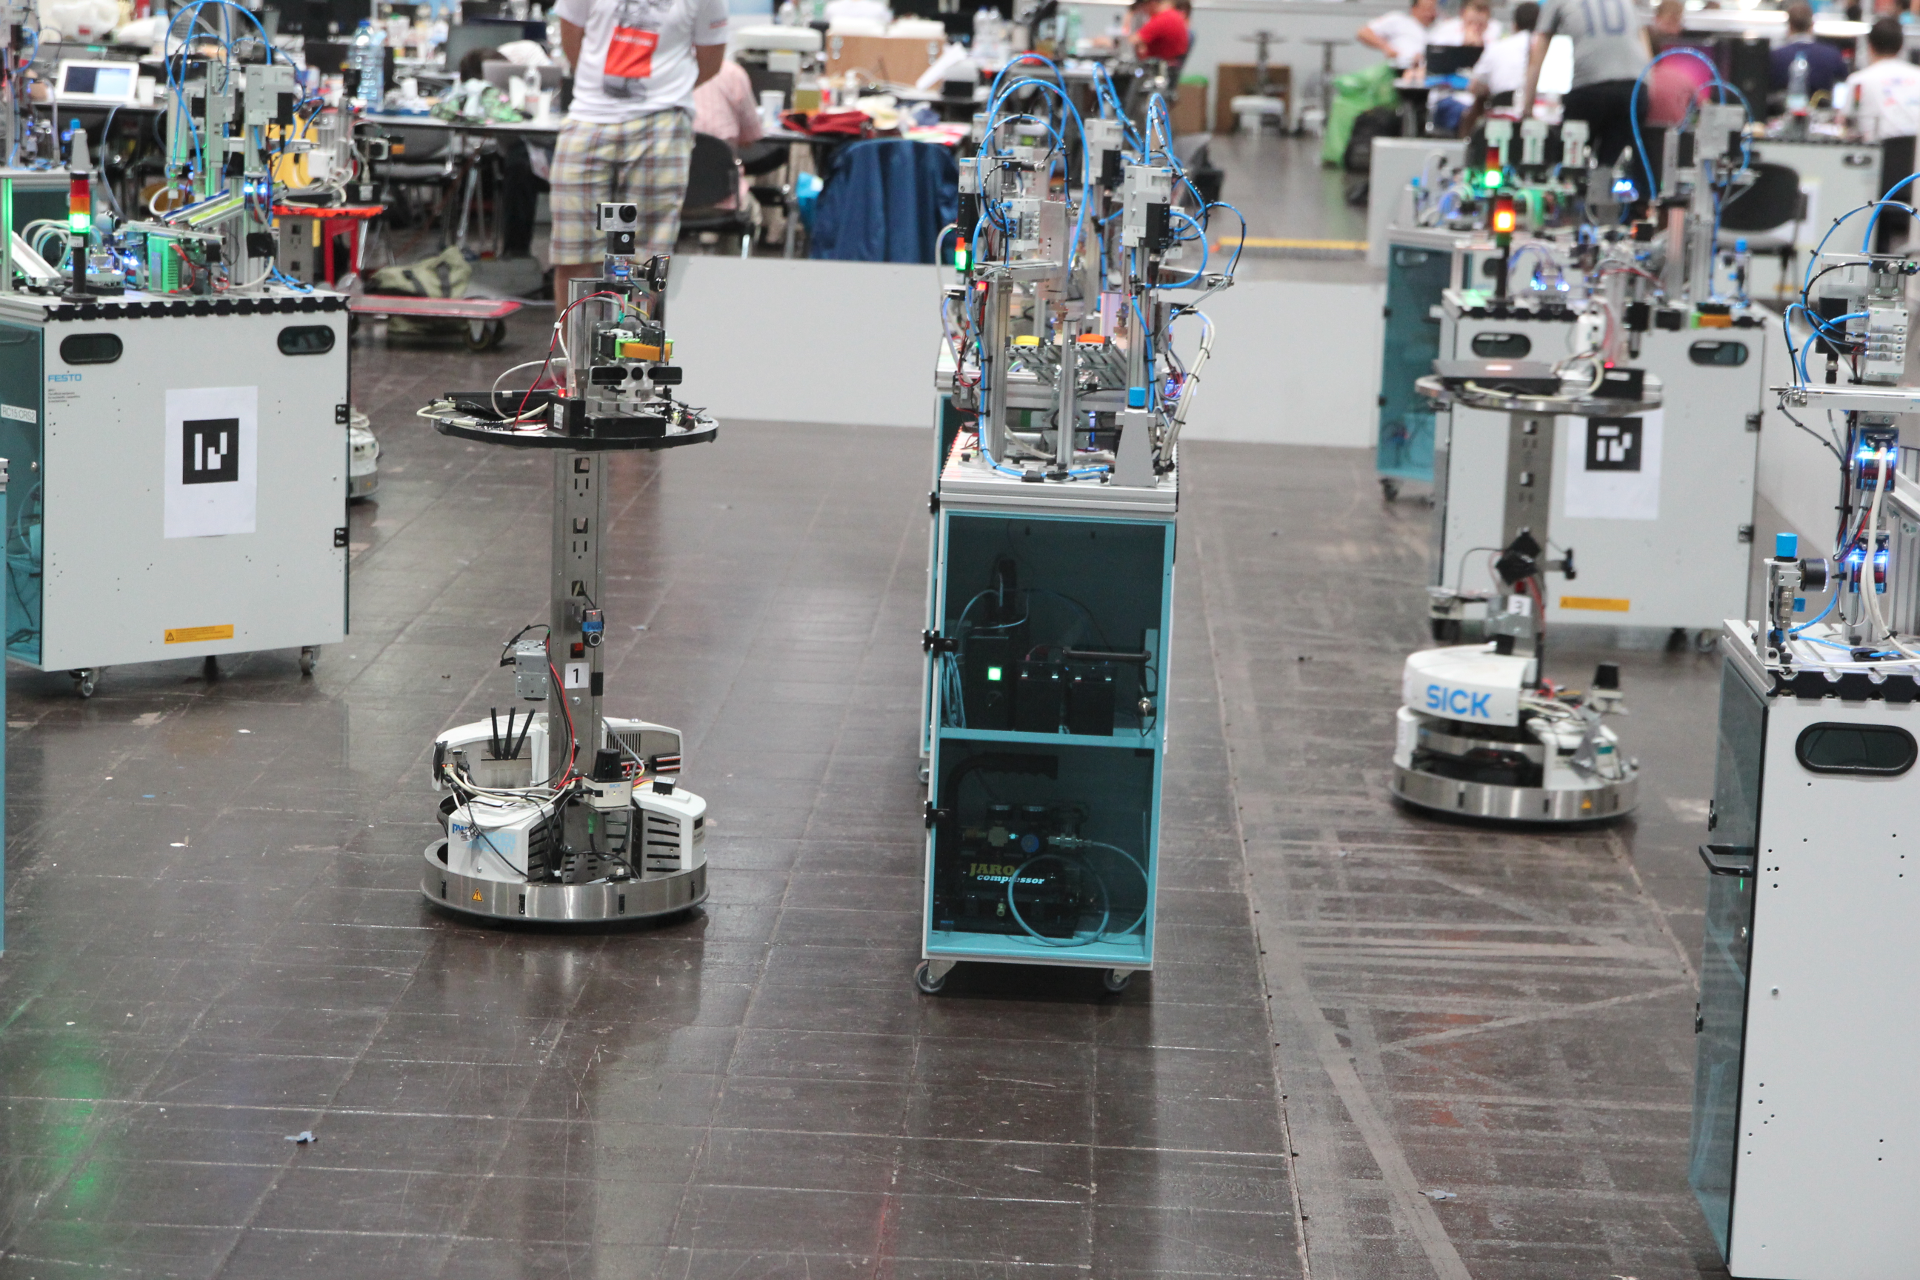
\includegraphics[width=\textwidth]{../thesis/img/rcll-feld}
    \begin{itemize}
    \item Store and reason about world state
    \item Share information in multi-robot system
    \end{itemize}
%% share knowledge to collaborate
    \end{column}
    \begin{column}{0.5\textwidth}
    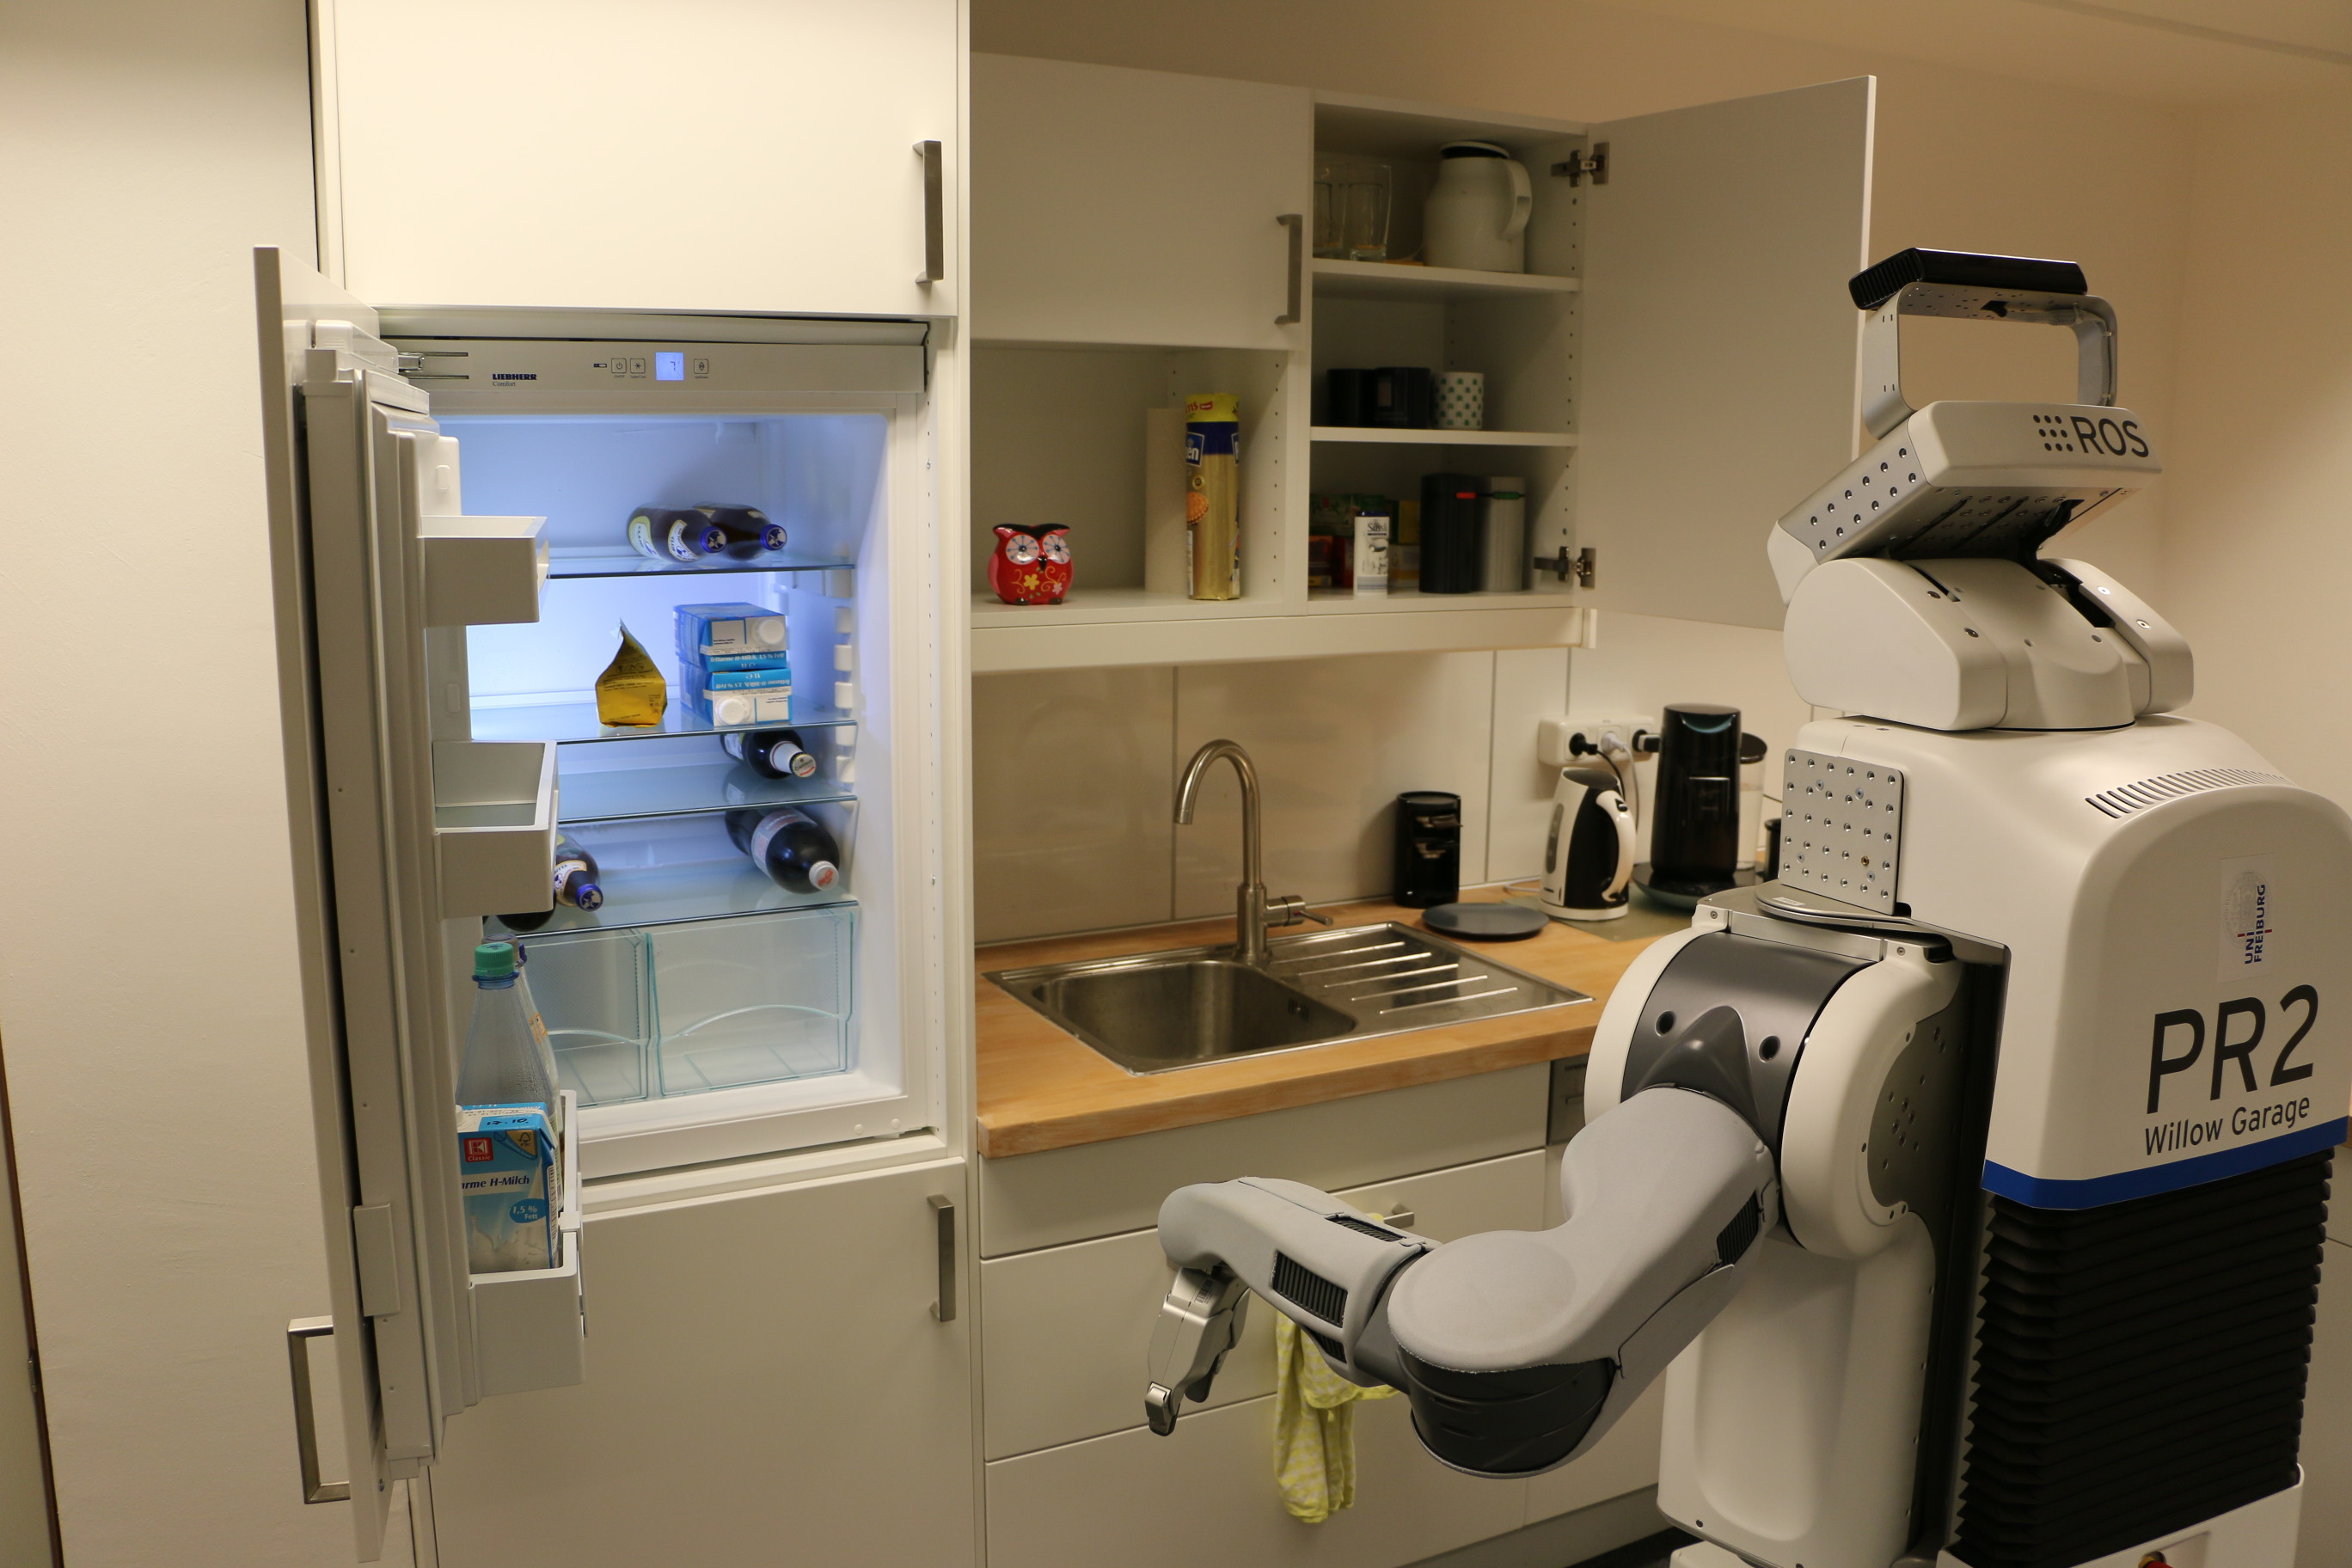
\includegraphics[width=\textwidth]{../thesis/img/pr2-kbsg-kitchen}
    \begin{itemize}
    \item Remember object sights
    \item Persistent storage
    \item Consistent information base for different components
    \end{itemize}
    \end{column}
  \end{columns}
\end{frame}

\begin{frame}
  \frametitle{Robot Memory Goals}
  \begin{itemize}
  \item Flexible storage and retrieval % generic
  \item Spatio-temporal grounding
  \item Persistent storage
  \bigskip
  \item Memory sharing between knowledge-based systems
  %\item Special views for different components
  \item Distributed memory for multi-robot systems
  \bigskip
  \item Computation on demand (\emph{Computables})
  \item Notification about updates (\emph{Triggers})
  %\item Human interface and visualization
  \end{itemize}
\end{frame}


\section{Background}
\begin{frame}[plain]
  \tableofcontents[currentsection]
\end{frame}
\addtocounter{framenumber}{-1}

\begin{frame}
  \frametitle{Application Domains}
  \begin{columns}
    \begin{column}{0.5\textwidth}
      \centering
      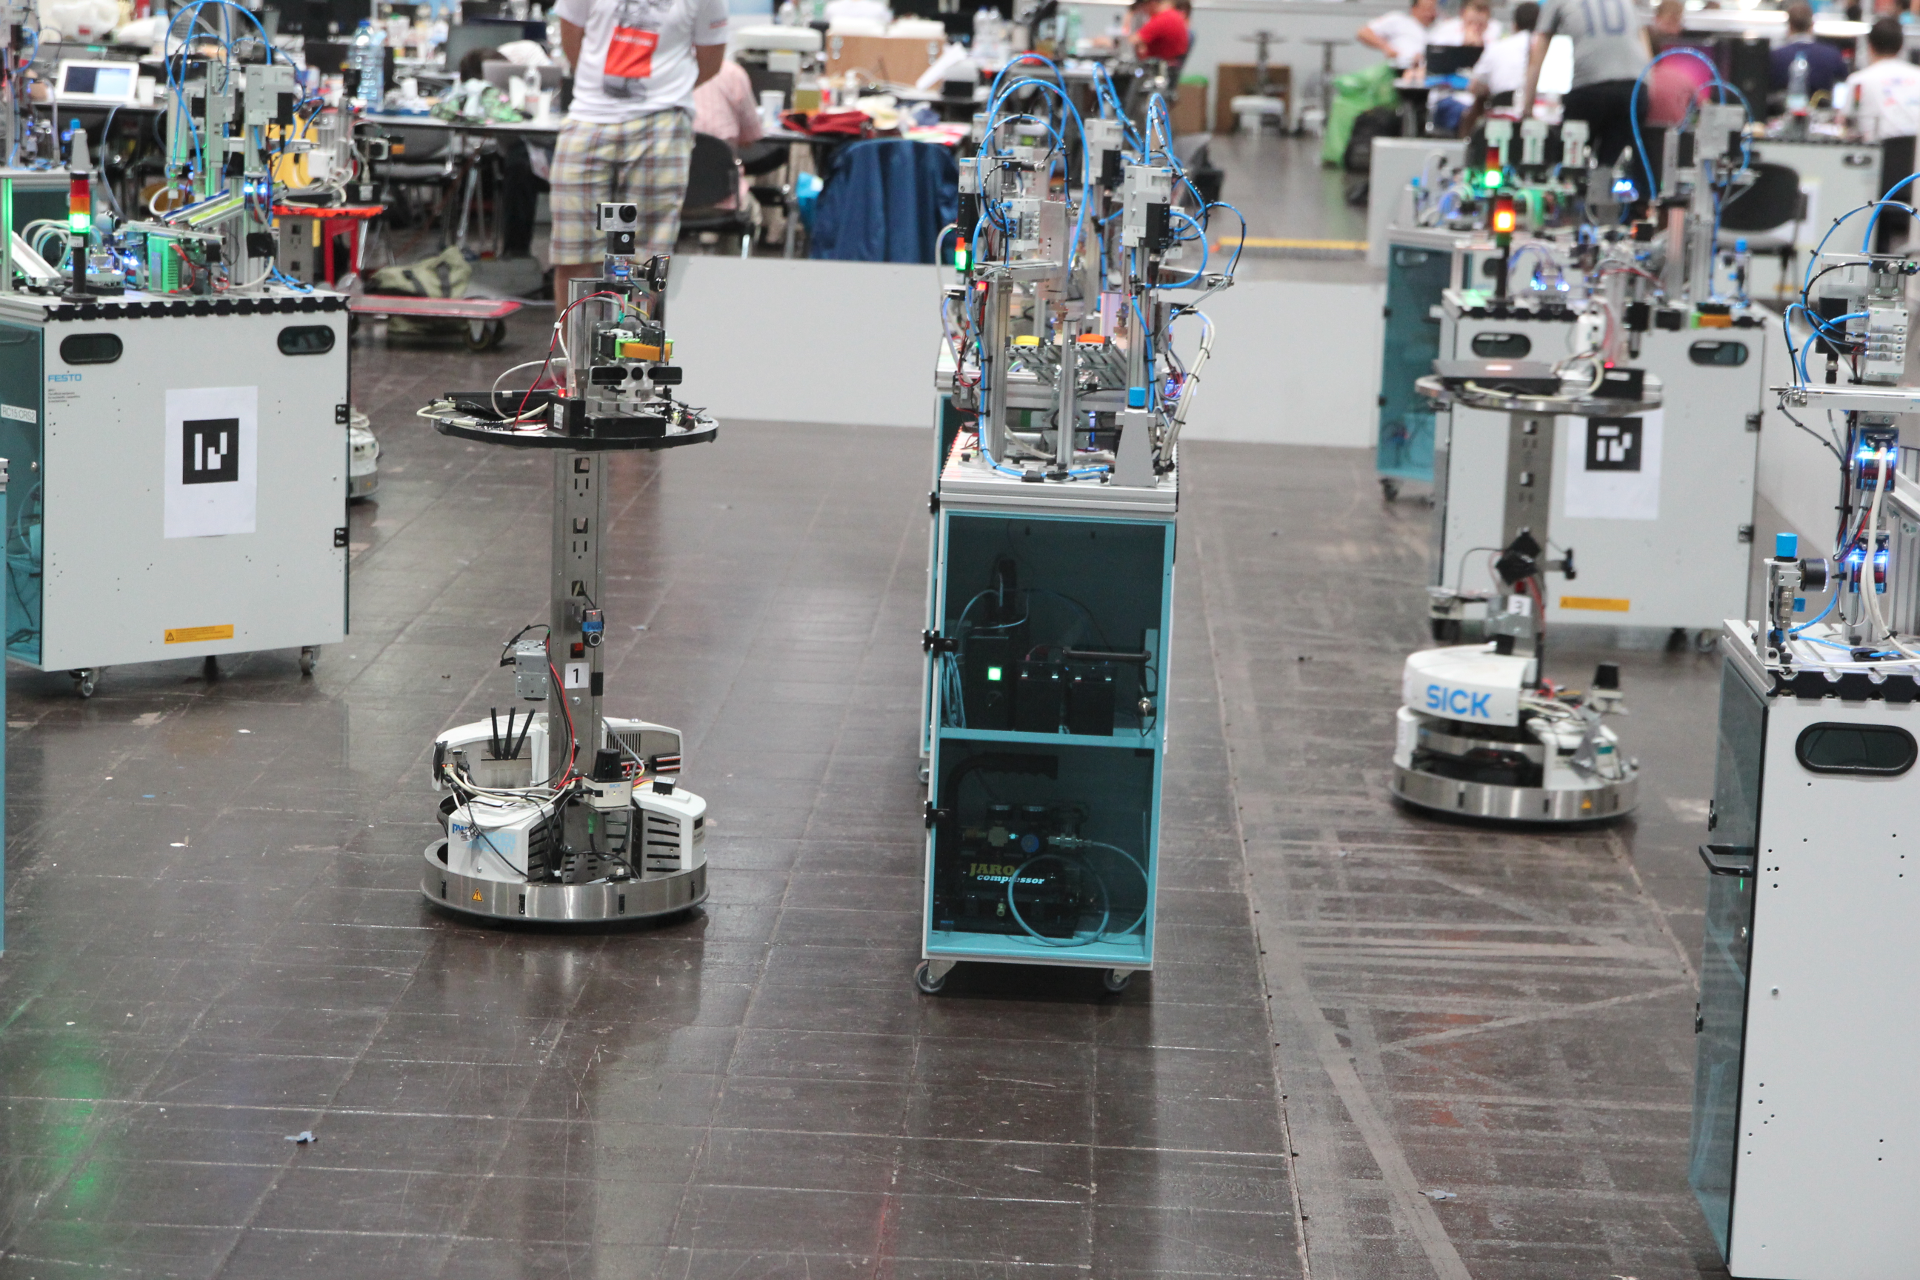
\includegraphics[width=0.7\textwidth]{../thesis/img/rcll-feld}
  \begin{description}[]
  \item[RoboCup Logistics League] \hfill \\
    \begin{itemize}
    \item Production logistics\\ in smart factory
    \item Share world model
    \begin{itemize}
    \item between robots
    \item between global planner and reasoner executive
    \end{itemize}
    \end{itemize}
  \end{description}
    \end{column}
    \begin{column}{0.5\textwidth}
    \centering
    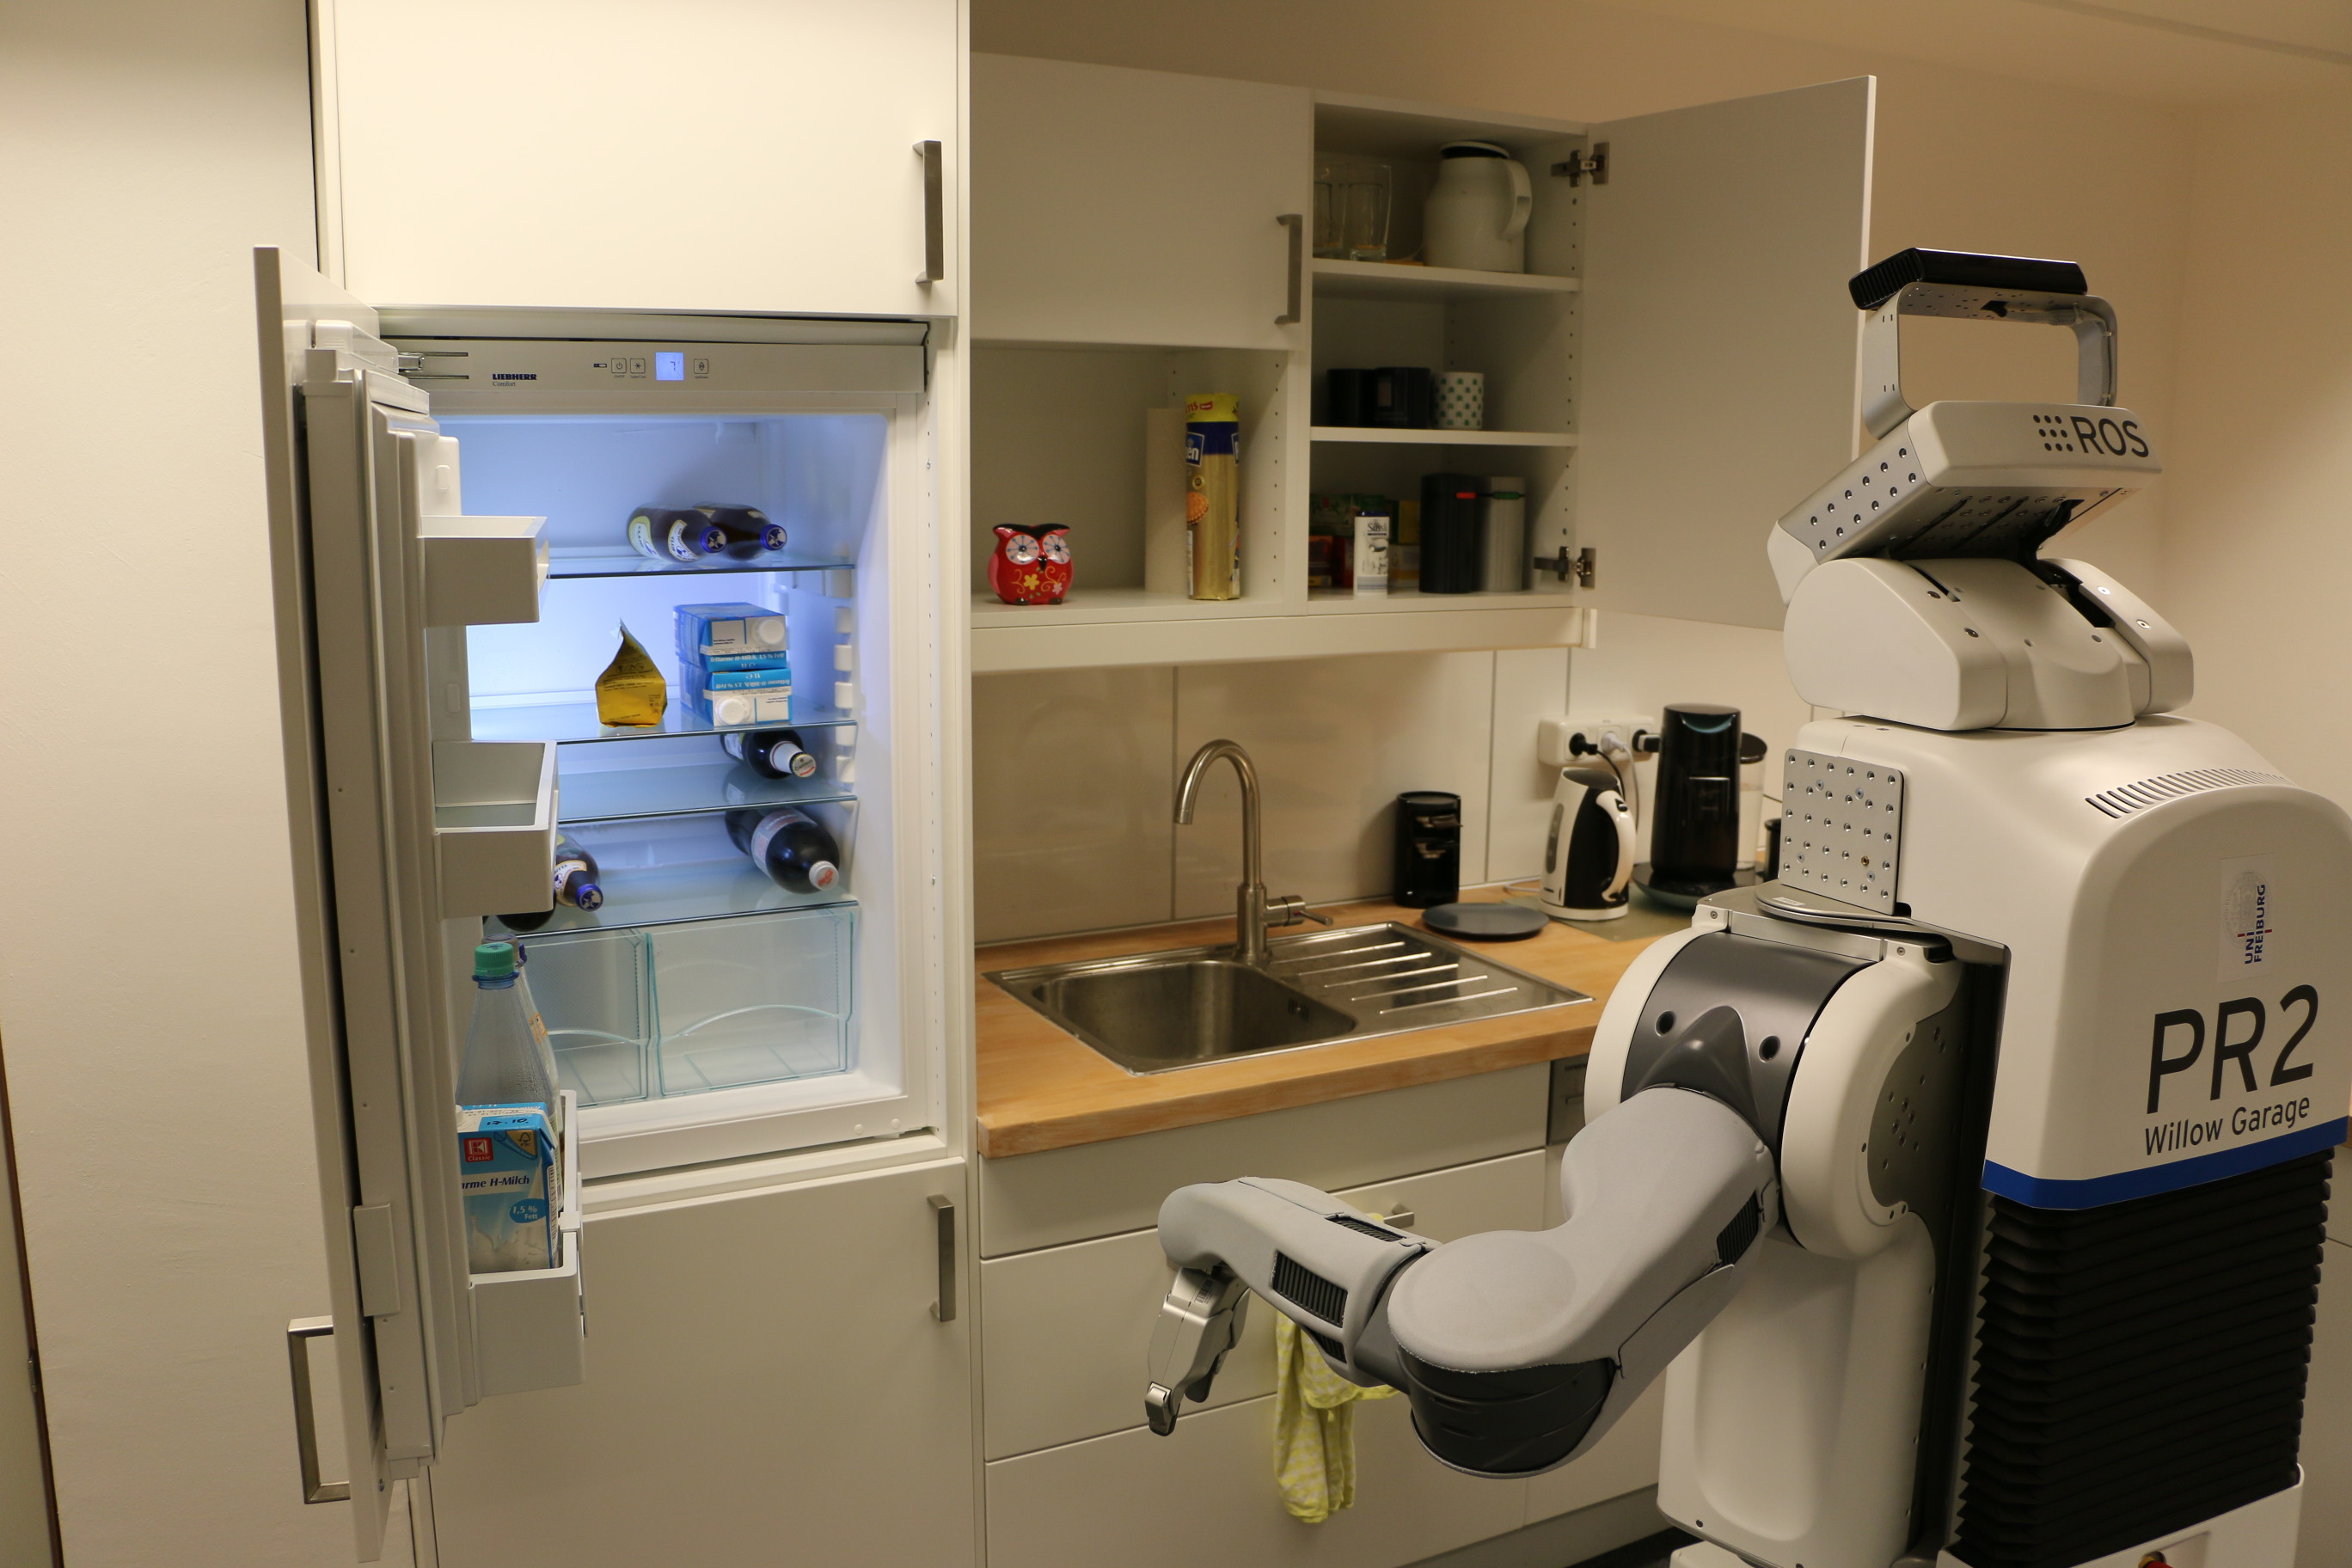
\includegraphics[width=0.7\textwidth]{../thesis/img/pr2-kbsg-kitchen}
  \begin{description}[]
  \item[RoboCup@Home] \hfill \\
    \begin{itemize}
    \item Domestic service robots
    \item Collect knowledge about concrete environment
    \item Hybrid reasoning with spatio-temporal knowledge
    \item Persistent storage
    \end{itemize}
  \end{description}    
    \end{column}
  \end{columns}
%TODO: already intorduce evaluation scenario here?
  \end{frame}

\begin{frame}
  \frametitle{Planners and Reasoners in Fawkes}
  \begin{columns}
  \begin{column}{0.83\linewidth}
  \begin{description}[]
  \item[CLIPS Rules Engine] \hfill \\
  \begin{itemize}
  \item First-Order Logic forward chaining system
  \item Fact base and condition-action rules
  \item[$\Rightarrow$] Used for world model reasoning and\\ execution monitoring
  \end{itemize}
  \item[Planning Domain Definition Language (PDDL)]%<uncover@2->
    \hfill \\
  \begin{itemize}
  \item Standardized language for planning problems
  \item Find action sequence through heuristic search
  \item[$\Rightarrow$] Used for finding global plans
  \end{itemize}
  \item[Motion Planners]%<uncover@3->
    \hfill \\
  \begin{itemize}
  \item Robot arm and locomotion collision avoidance
  \item Depend on geometric data
  \end{itemize}
  \end{description}
  \end{column}
  \begin{column}{0.17\linewidth}
  
\includegraphics[width=\textwidth]{../thesis/img/CLIPS}
  \vspace{3.4cm}
  %\pause\pause
  
\includegraphics[width=\textwidth]{../thesis/img/openrave}
  \end{column}
  \end{columns}
\end{frame}

\section{Related Work}
\begin{frame}[plain]
  \tableofcontents[currentsection]
\end{frame}
\addtocounter{framenumber}{-1}

\begin{frame}
  \frametitle{Robot Information Storage Systems}
  \begin{description}[]
  \item[KnowRob~\cite{KnowRob}]%<uncover@1->
    \hfill \\
    \begin{itemize}
    \item Common sense reasoning with ontologies
          %explain with example (graph, rdf, milk)
    \item Virtual knowledge base to interface perception
    \item Based on Prolog
    \end{itemize}
  \end{description}
  \begin{description}[]
  \item[OpenRobots Ontology~\cite{Oro}]%<uncover@2-> 
    \hfill \\
    \begin{itemize}
    \item Common sense reasoning with ontologies
    \item Events notifying about changes
    \item Based on  Java
    \end{itemize}
  \end{description}
  \begin{block}{}%<uncover@3->
  \begin{itemize}
  \item Not applicable for multi-robot systems
  \item Scalability, efficiency concerns % because storage is interwined with reasoning
  \item Missing events / computation on demand
  \end{itemize}
  \end{block}
\end{frame}

\begin{frame}[fragile]
  \frametitle{Document Orientation}
  \begin{itemize}
  \item Documents: Sets of key-value pairs
    %keys unique, different value types
  \item Java Script Object Notation (JSON)
    \begin{lstlisting}[style=SmallJSON,linewidth=8.5cm,
      label=lst:json,
      framexleftmargin=1pt, xleftmargin=0pt,
      morekeywords={}, numbers=none]
      {
        "key": "value",
        "subdocument": {"x":3, "y":1},
        "array": [{"n":0.1},{"n":2}]
      }
    \end{lstlisting}
  \item Denormalized (information bundled in documents)
  \item Schema free
  \end{itemize}
  \begin{itemize}
  \item[$\Rightarrow$] Allows generic, flexible, and distributable robot memory
  \end{itemize}
\end{frame}

\begin{frame}[fragile]
  \frametitle{MongoDB Database System}
  \hfill
\includegraphics[width=0.3\textwidth]{../thesis/img/mongodb}
  \begin{itemize}
    \item Scalable and widely used
    \item Query language with aggregation, MapReduce, JavaScript % powerful query features
\begin{lstlisting}[style=SmallJSON,linewidth=8.5cm,
  framexleftmargin=2pt, xleftmargin=10pt,
 morekeywords={}, numbers=none]
db.environment.find(
  { object: "cup", color: {$ne: "red"}})
\end{lstlisting}%$
    \item Collections group documents
    \item Indexing for fast querying
    \item Distributable with Replica Sets\\ %explain a bit (Primary, Secondary)
      Operations Log (Oplog) to forward changes
    \item Comparable good performance and scalability\\\cite{arango-vs-mongo,db-comparison}
  \end{itemize}
\end{frame}

\begin{frame}
  \frametitle{Related Work with MongoDB}
  \begin{description}
  \item[Robot Database with MongoDB~\cite{RoboDB}]%<uncover@1->
                \hfill \\
    \begin{itemize}
    \item Data logging for evaluation and fault analysis
    \item Generic and scalable storage with MongoDB
    \item Integration in Fawkes and ROS
    \end{itemize}
\bigskip
  \item[Extensions of  MongoDB]%<uncover@2->
                \hfill \\
    \begin{itemize}
    \item Triggers with replication Oplog~\cite{mongodb-trigger}
    %\item Multi-Master Replication~\cite{mongodb-multi-master}
    \end{itemize}
  \end{description}
\end{frame}


\section{Approach}
\begin{frame}[plain]
  \tableofcontents[currentsection]
\end{frame}
\addtocounter{framenumber}{-1}

\begin{frame}
  \frametitle{Terminology}
  \begin{description}
  \item[Documents] \hfill {\small $\{("object","cup"),("position",{\scriptstyle\{("x",8),("y",4)\}})\}$}\\
    \begin{itemize}
    \item Sets of key-value pairs (unique keys)
    \item Finitely nested sub-documents
    \end{itemize}
\bigskip
  \item[Robot Memory] \hfill \\
    \begin{itemize}
    \item Composed of database and computables
    \item Database: Set of documents
    \item Computables: Functions yielding sets of documents
    \end{itemize}
  \end{description}  
\end{frame}

\begin{frame}
  \frametitle{Computables}
  \only<1>{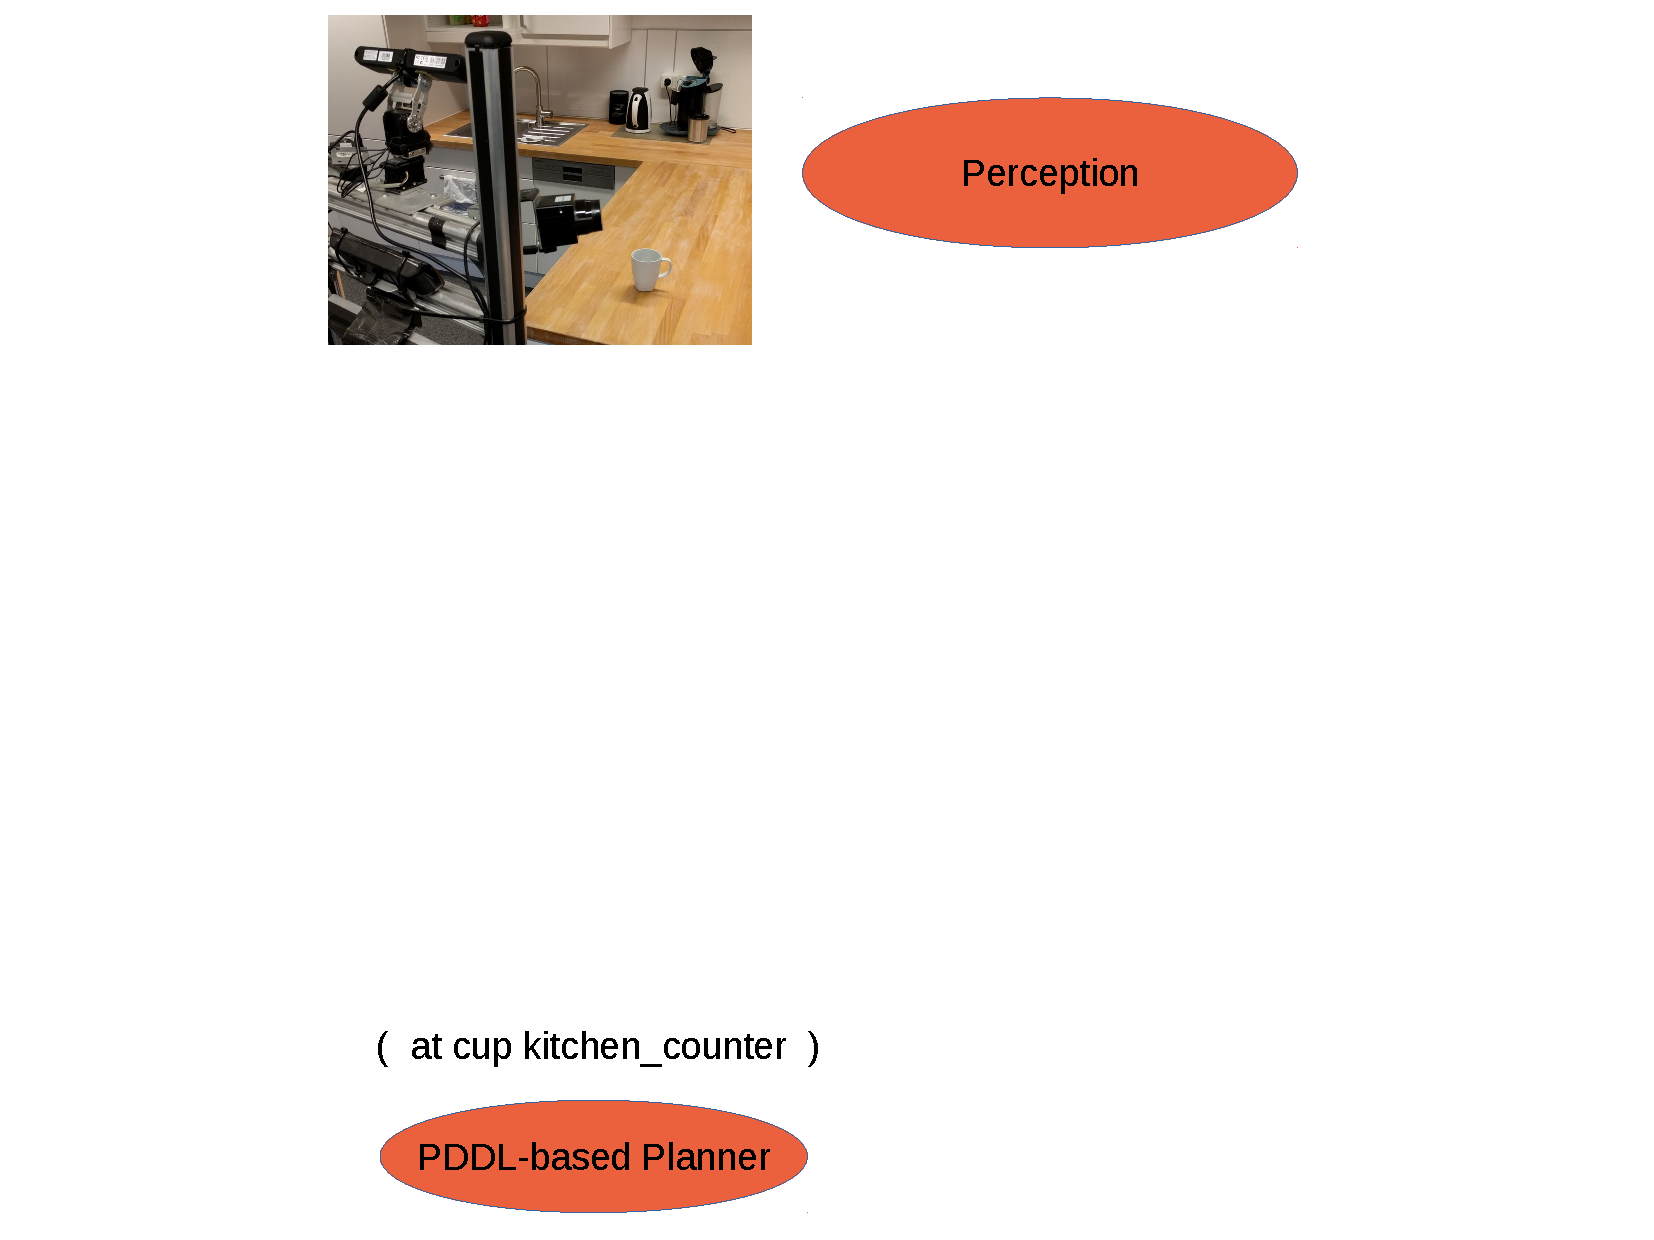
\includegraphics[width=1.03\textwidth]{../thesis/draw/computable-4.pdf}}
  \only<2>{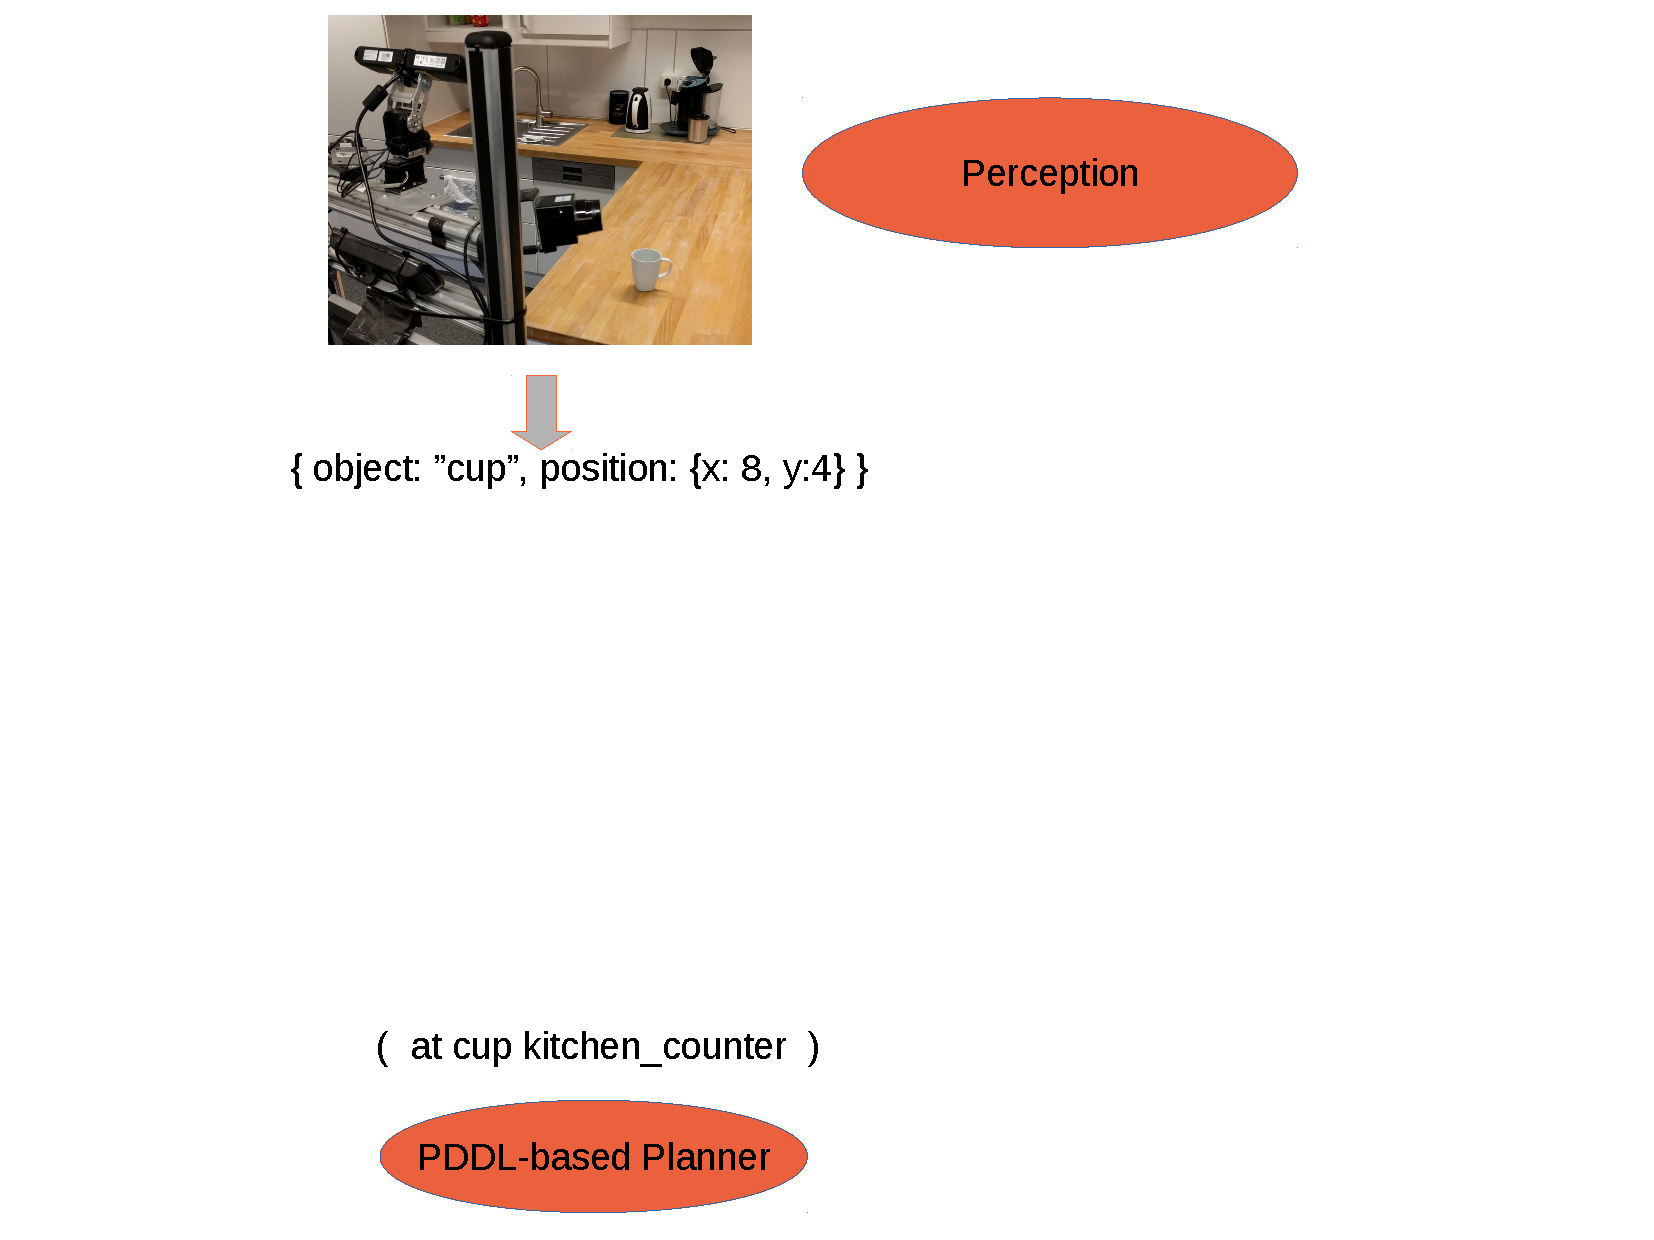
\includegraphics[width=1.03\textwidth]{../thesis/draw/computable-3.pdf}}
  \only<3>{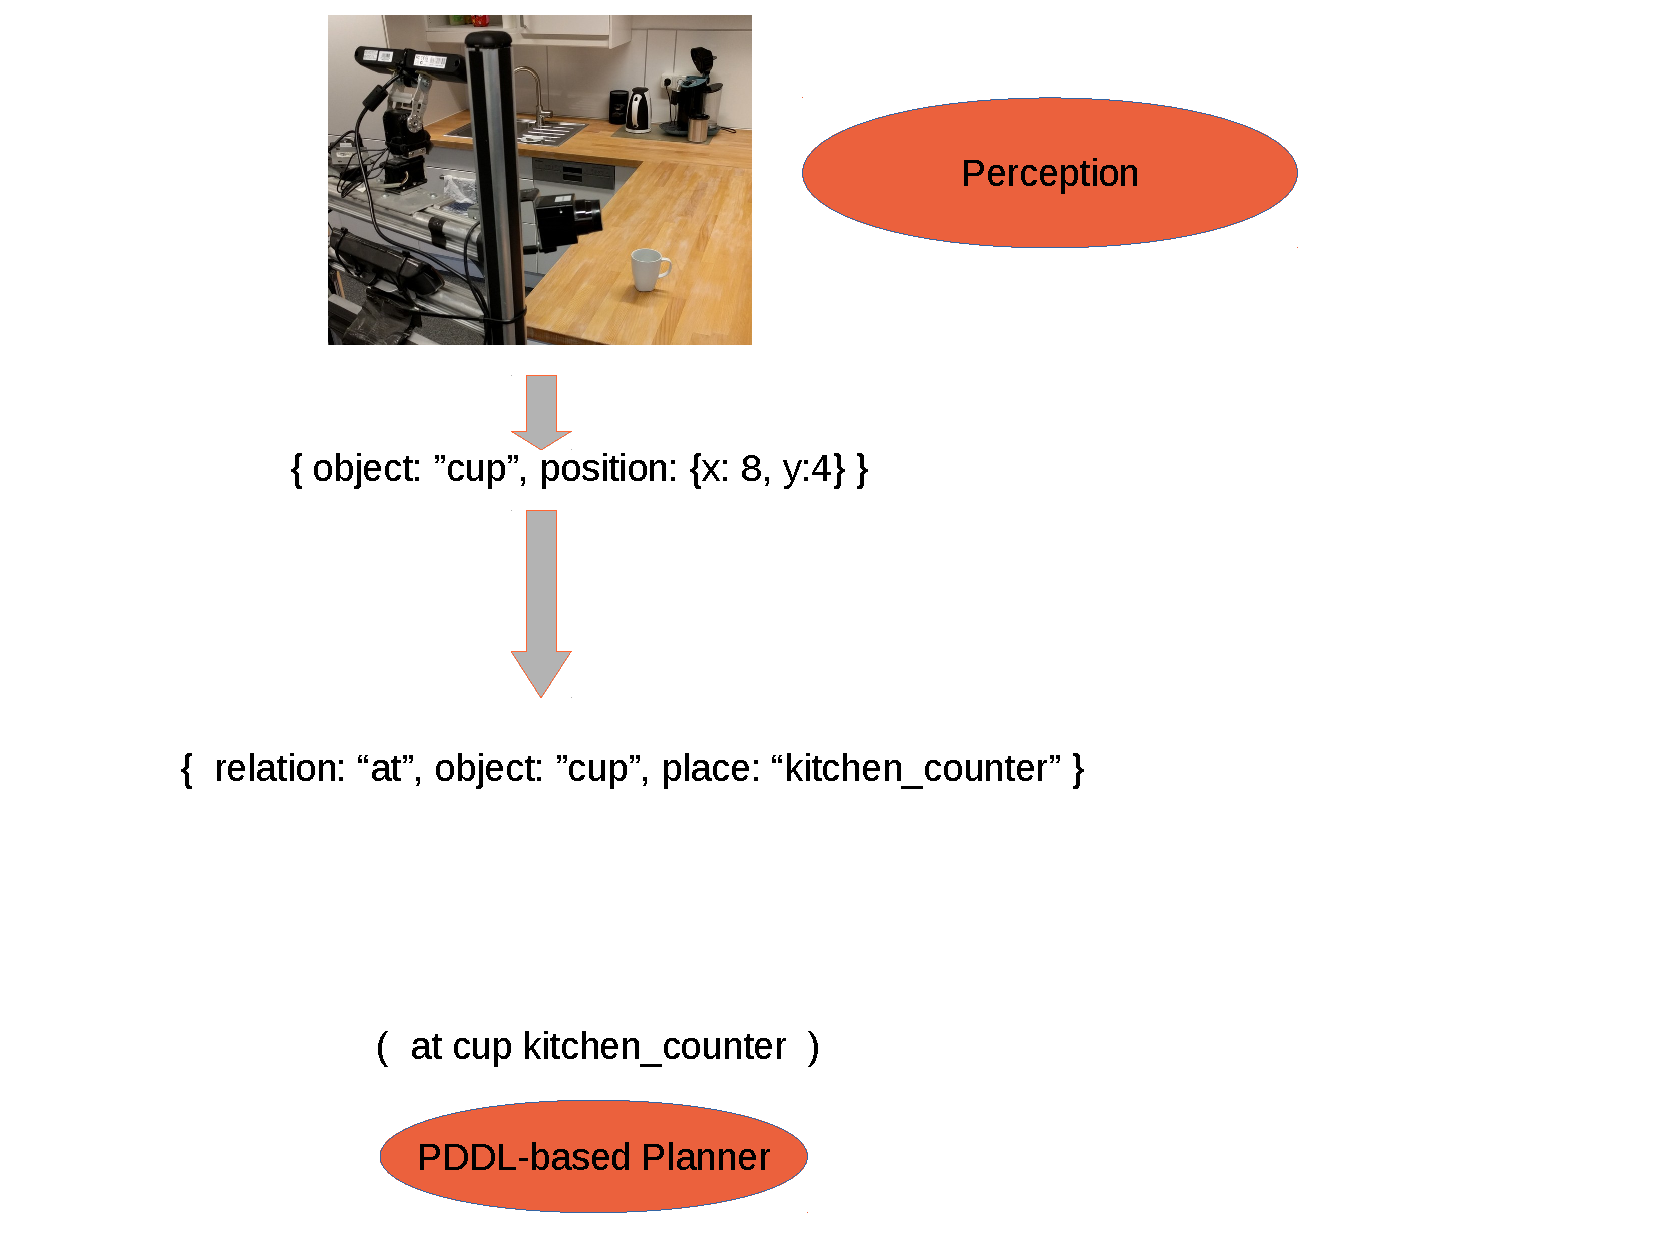
\includegraphics[width=1.03\textwidth]{../thesis/draw/computable-2.pdf}}
  \only<4>{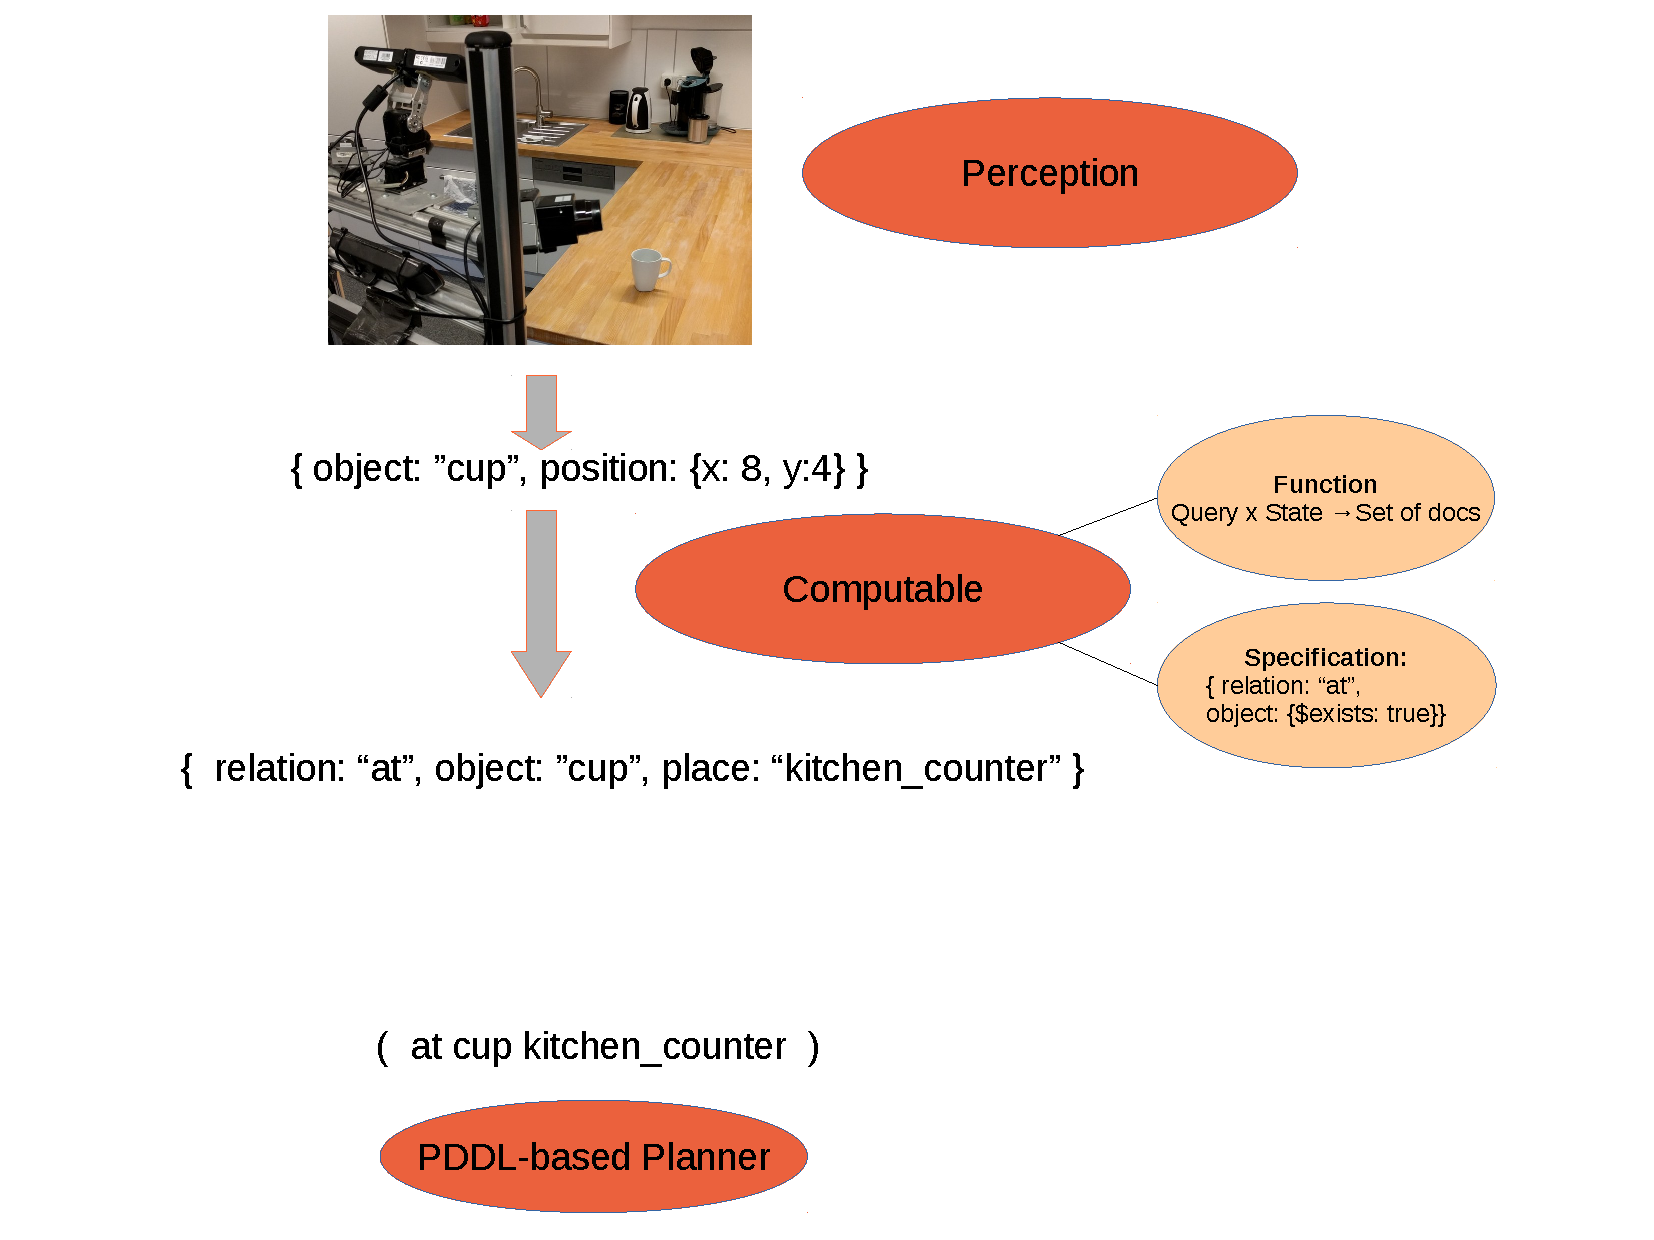
\includegraphics[width=1.03\textwidth]{../thesis/draw/computable-1.pdf}}
  \only<5>{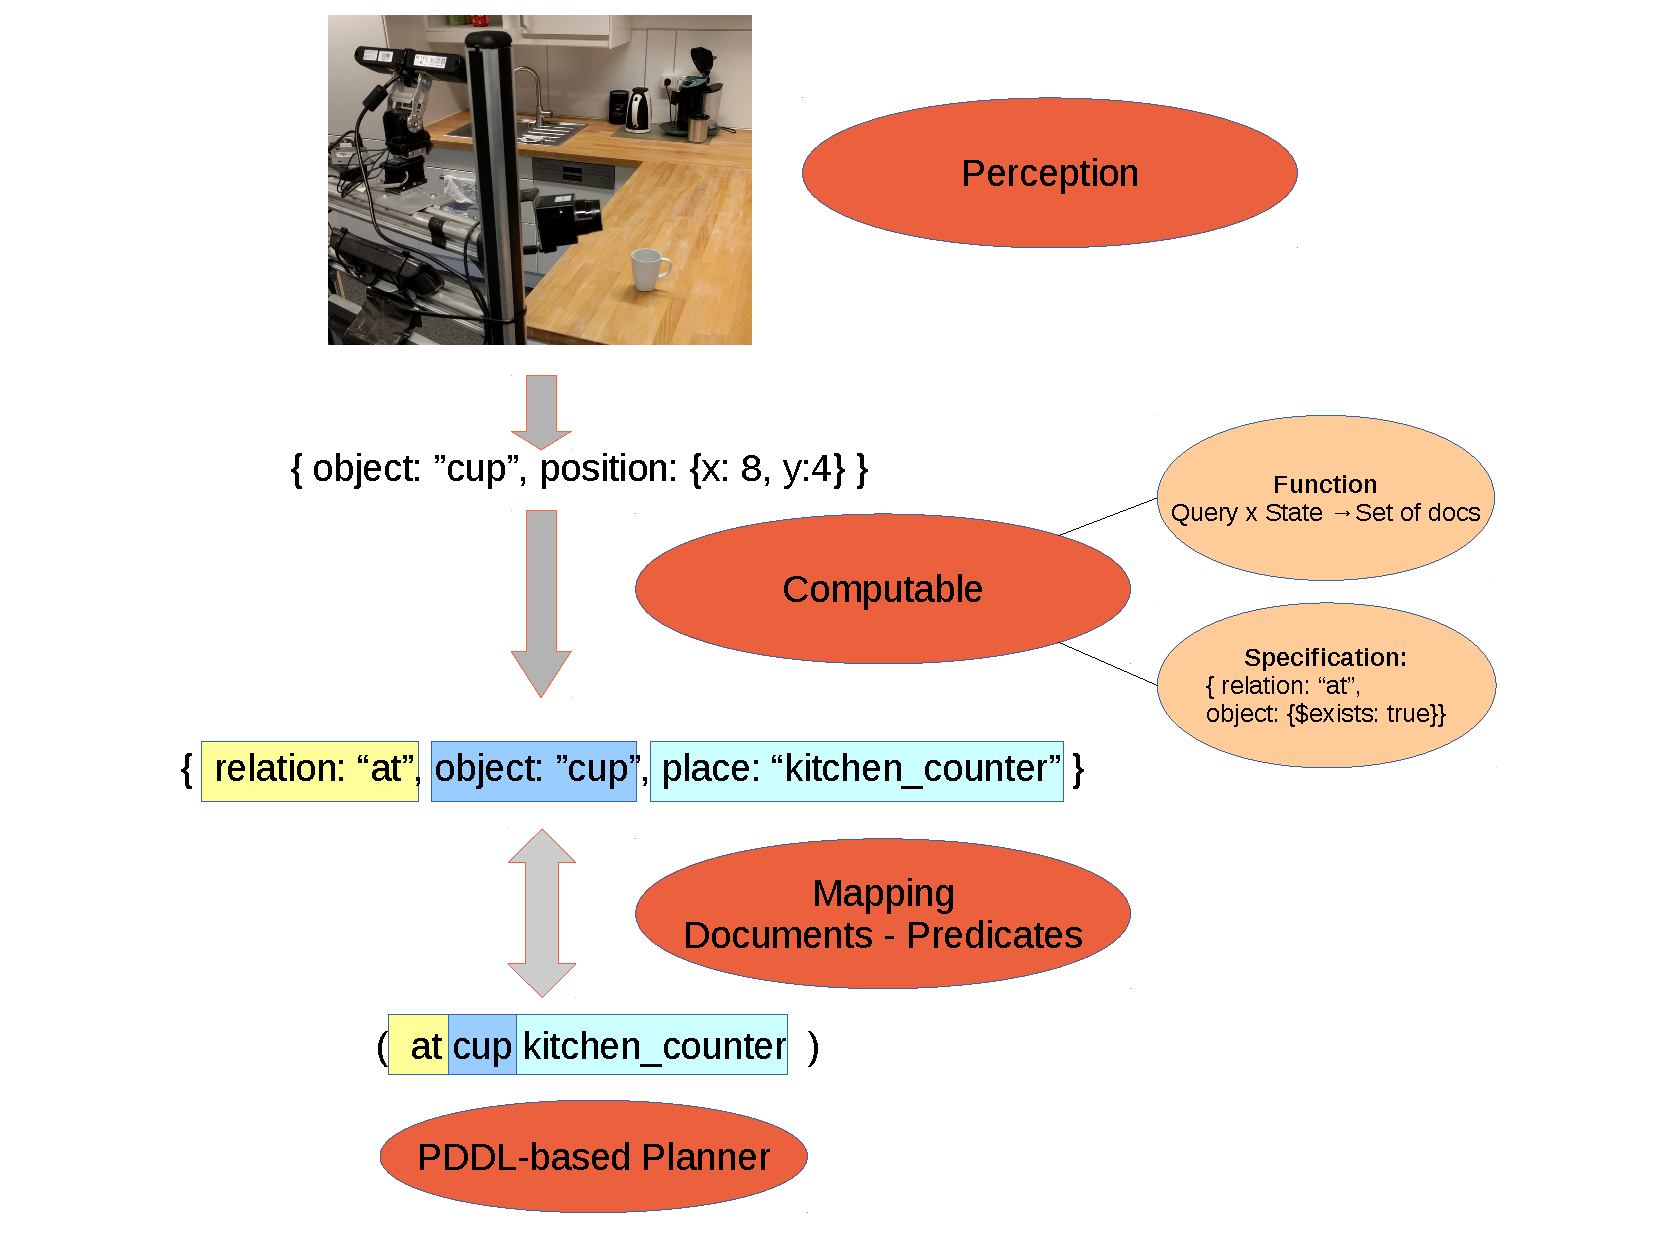
\includegraphics[width=1.03\textwidth]{../thesis/draw/computable.pdf}}
  \pause\pause\pause\pause
\end{frame}

\begin{frame}
  \frametitle{Triggers}
  \only<1>{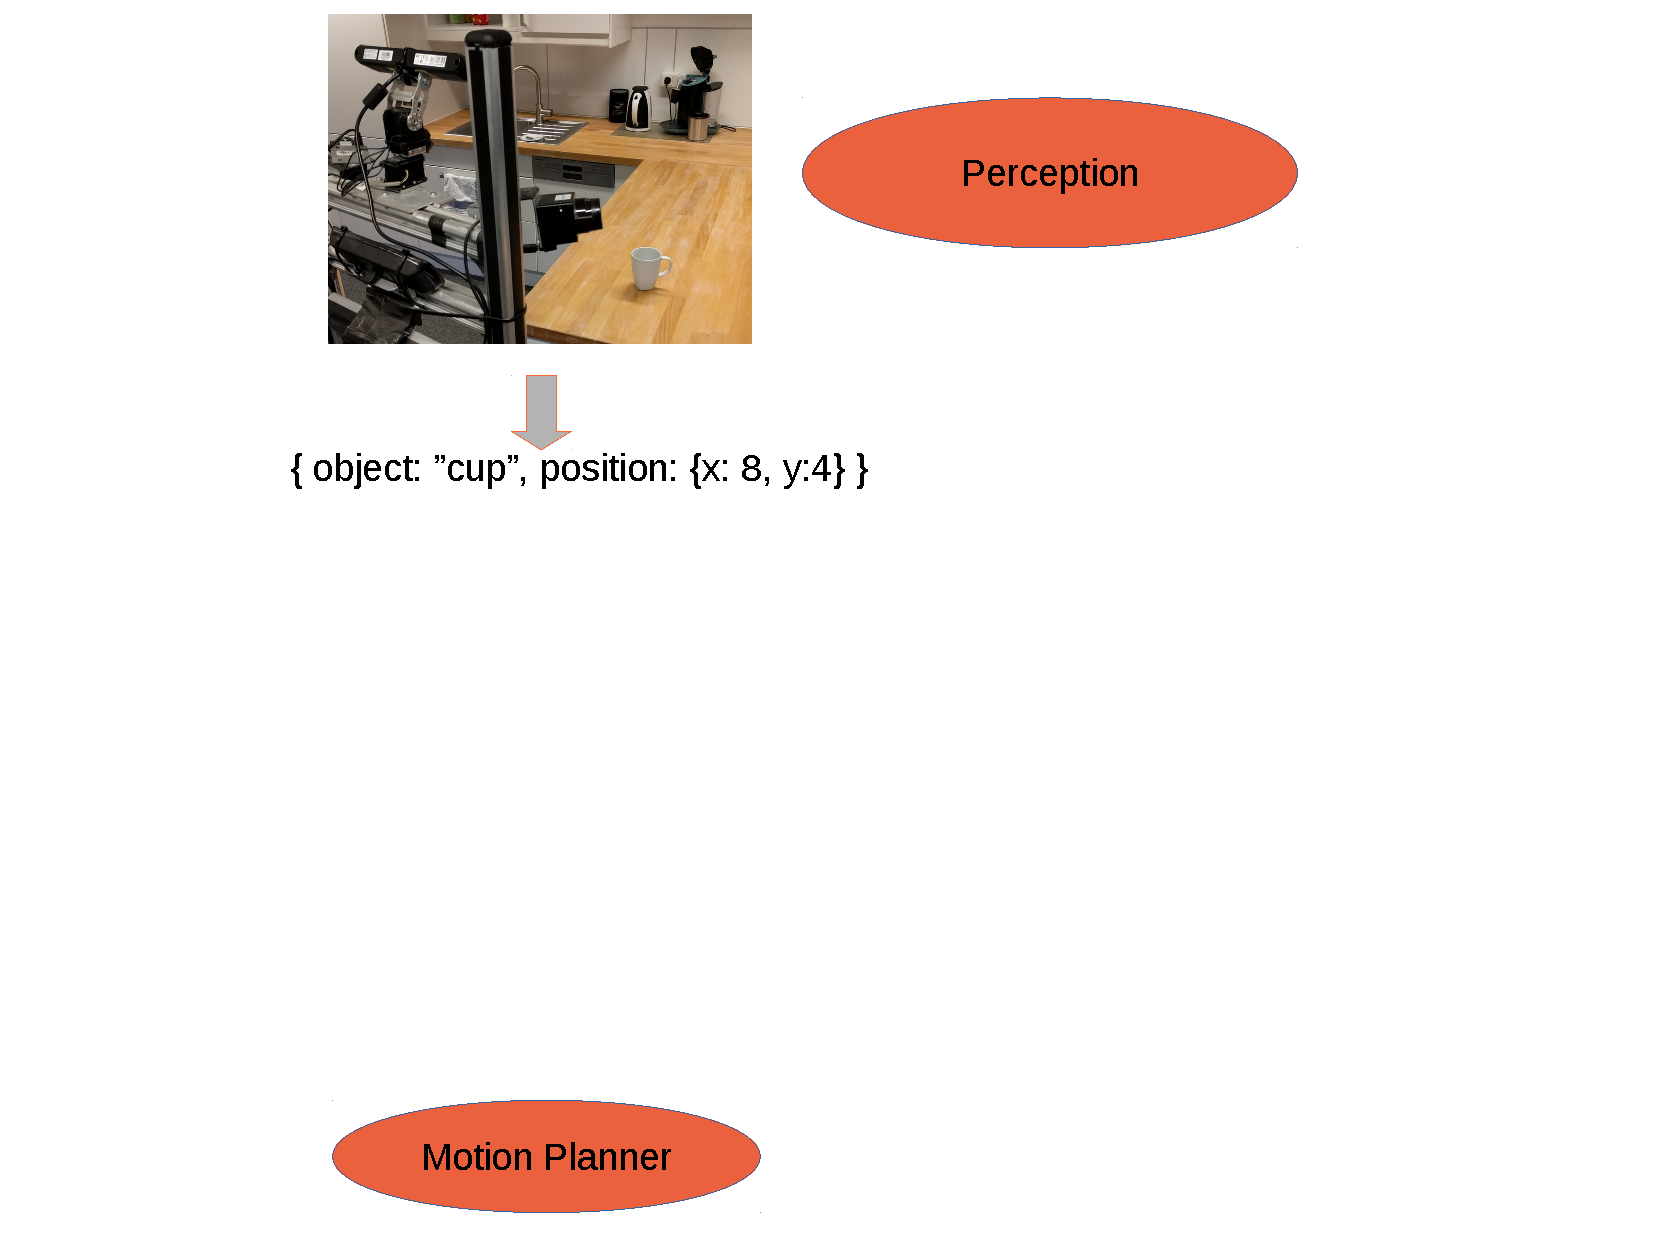
\includegraphics[width=1.03\textwidth]{../thesis/draw/trigger-5.pdf}}
  \only<2>{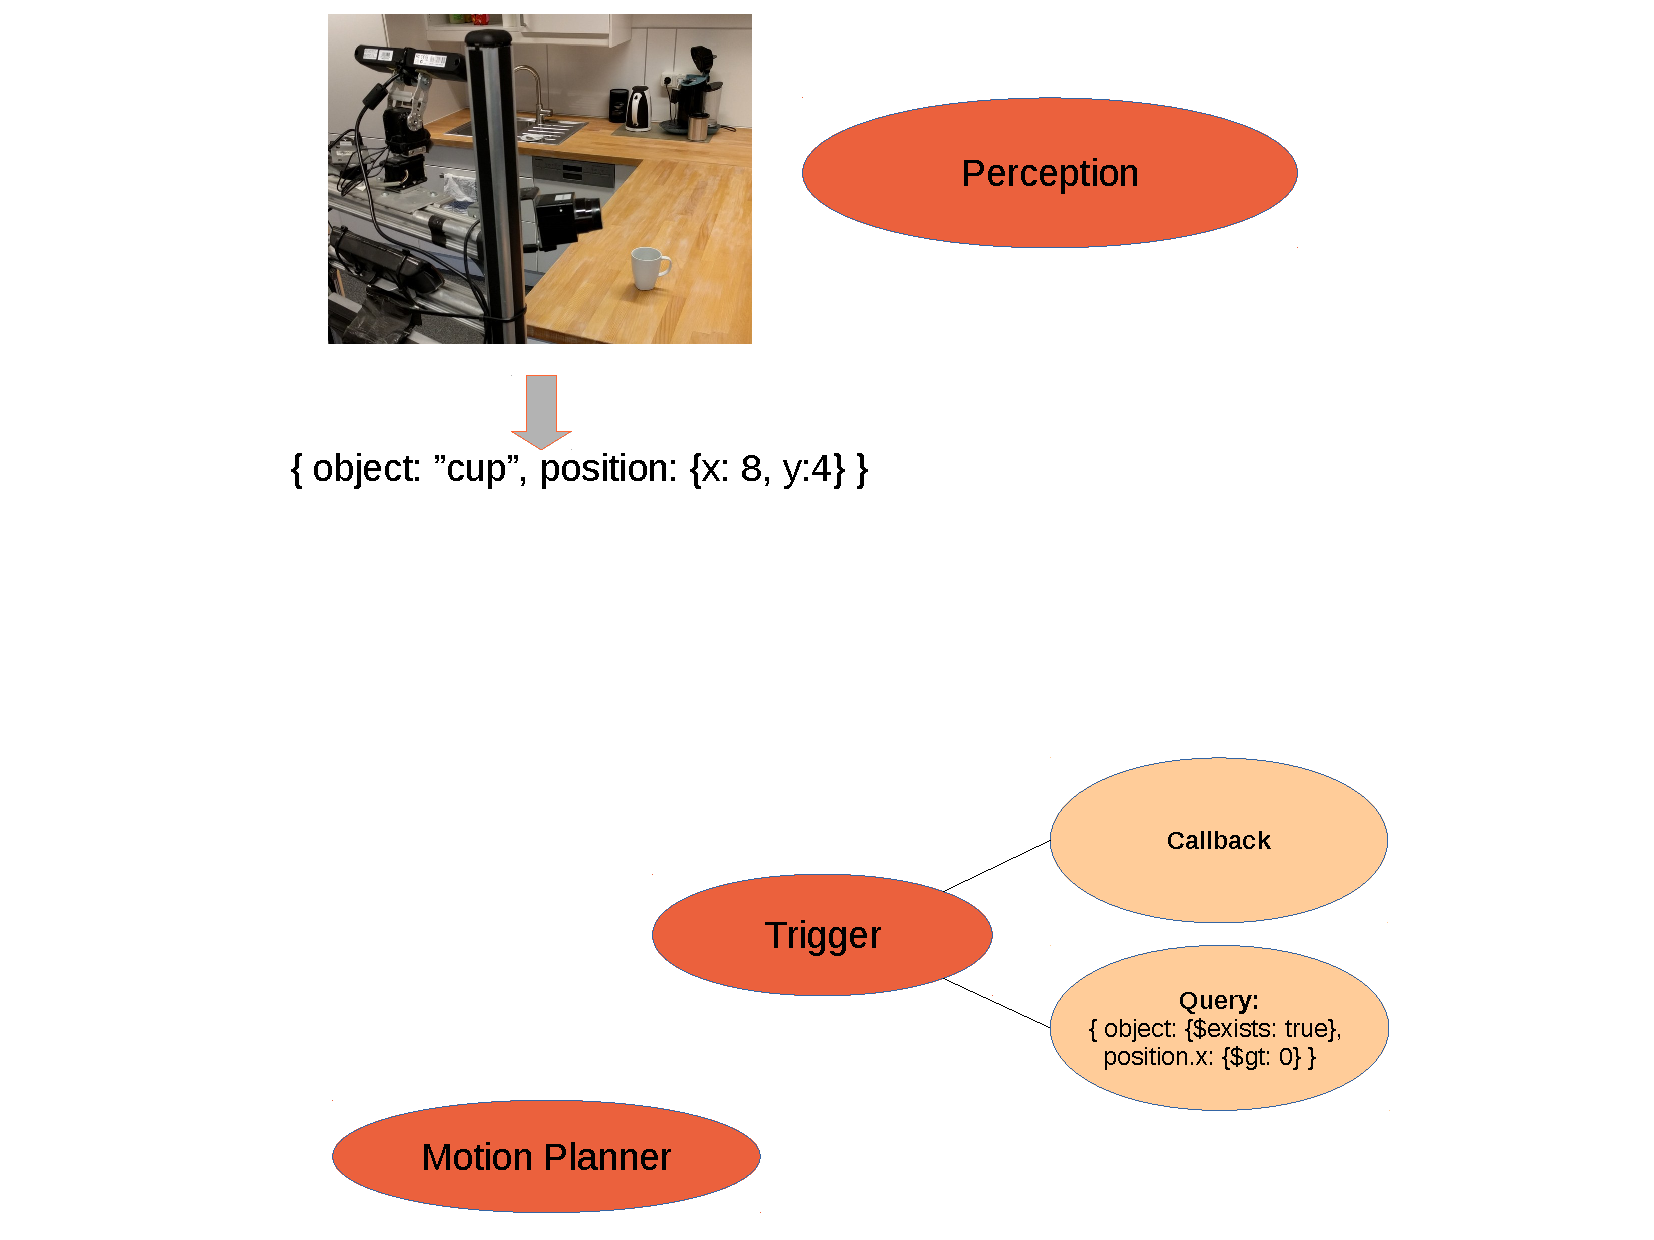
\includegraphics[width=1.03\textwidth]{../thesis/draw/trigger-4.pdf}}
  \only<3>{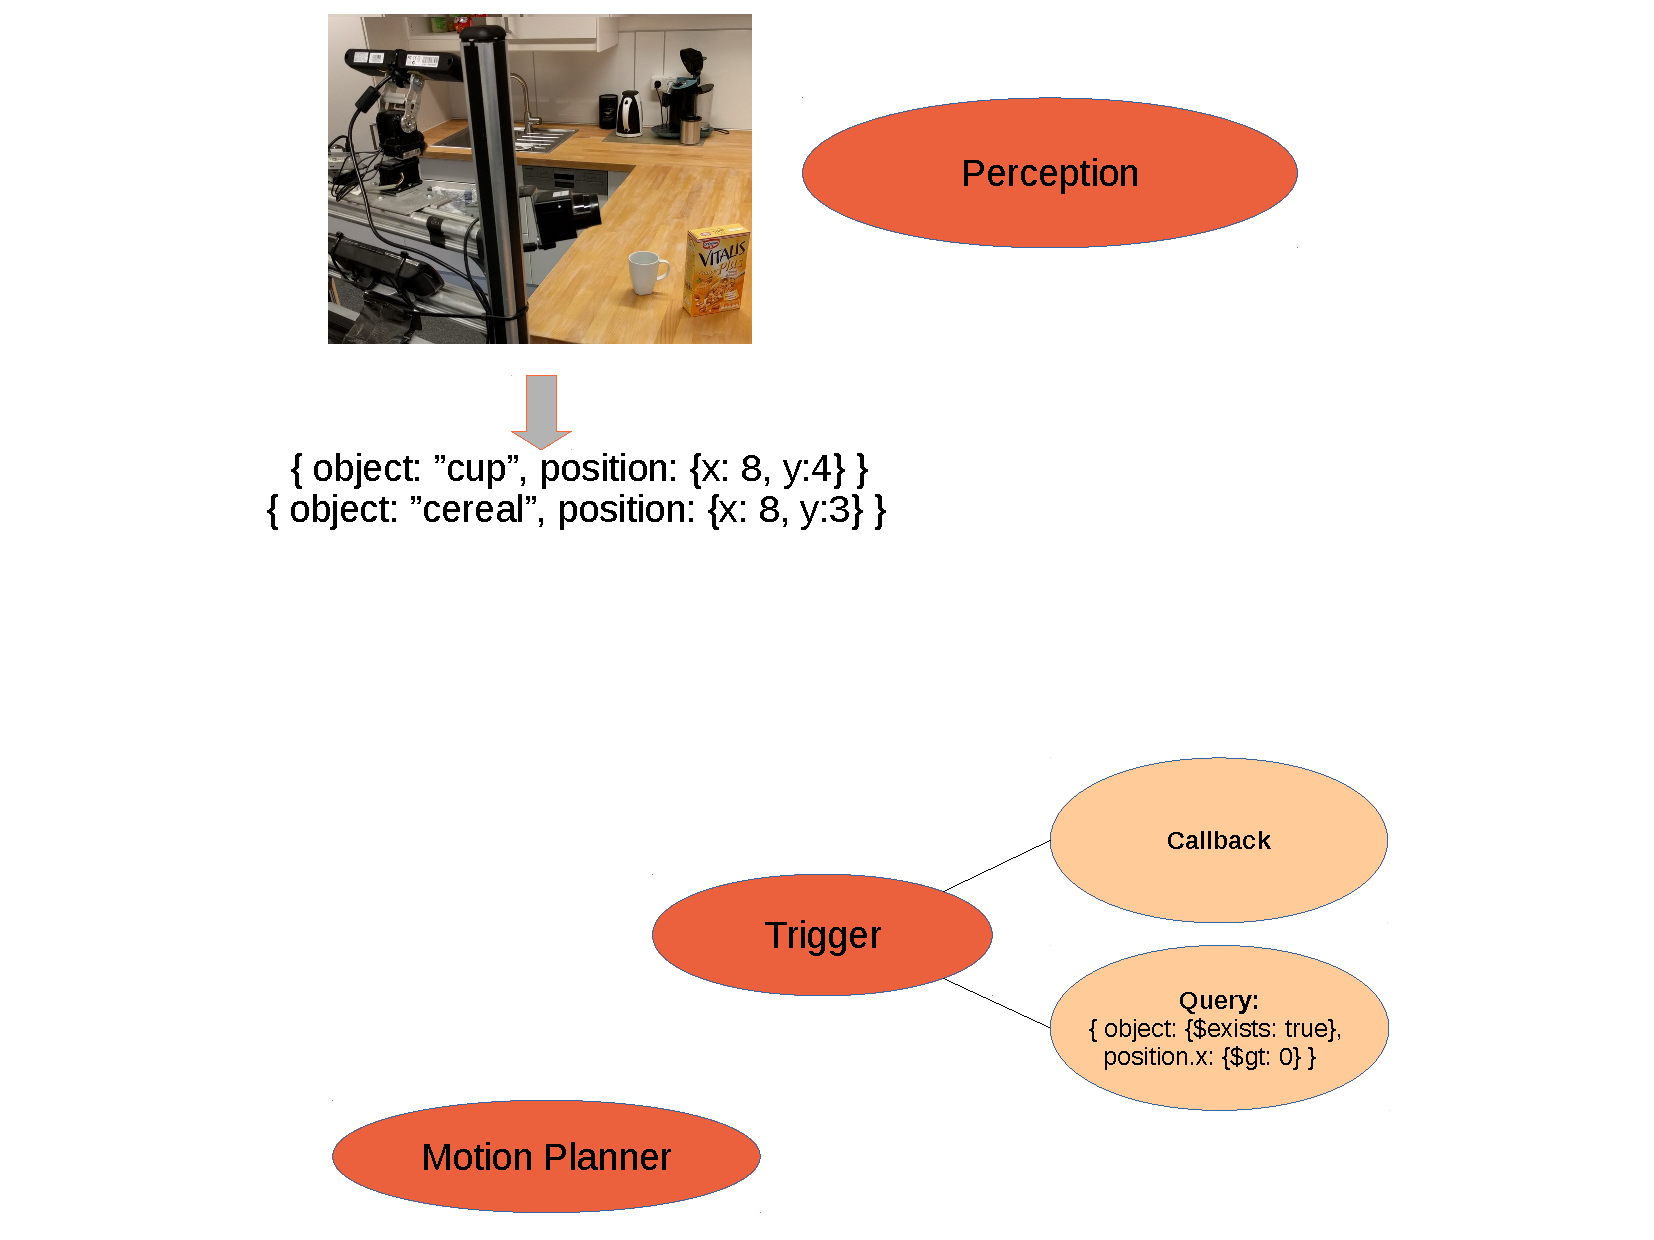
\includegraphics[width=1.03\textwidth]{../thesis/draw/trigger-3.pdf}}
  \only<4>{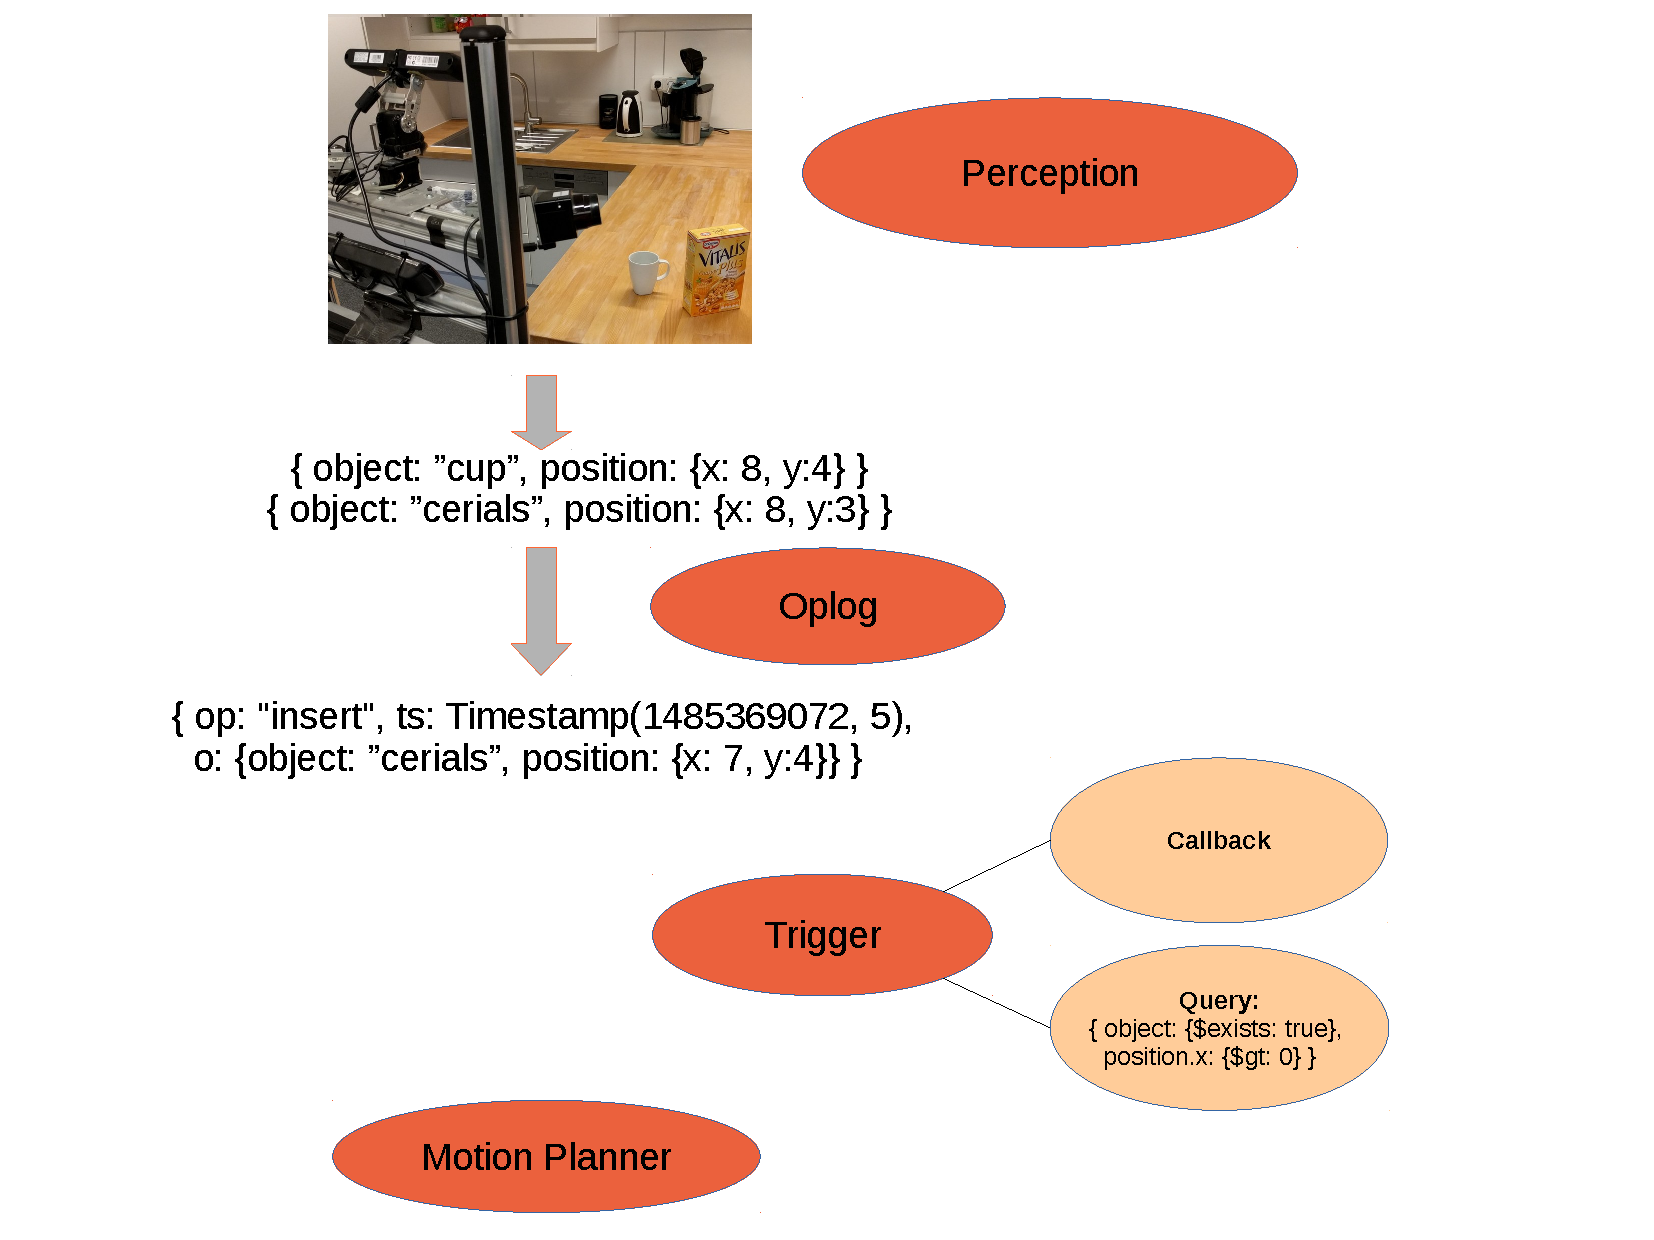
\includegraphics[width=1.03\textwidth]{../thesis/draw/trigger-2.pdf}}
  \only<5>{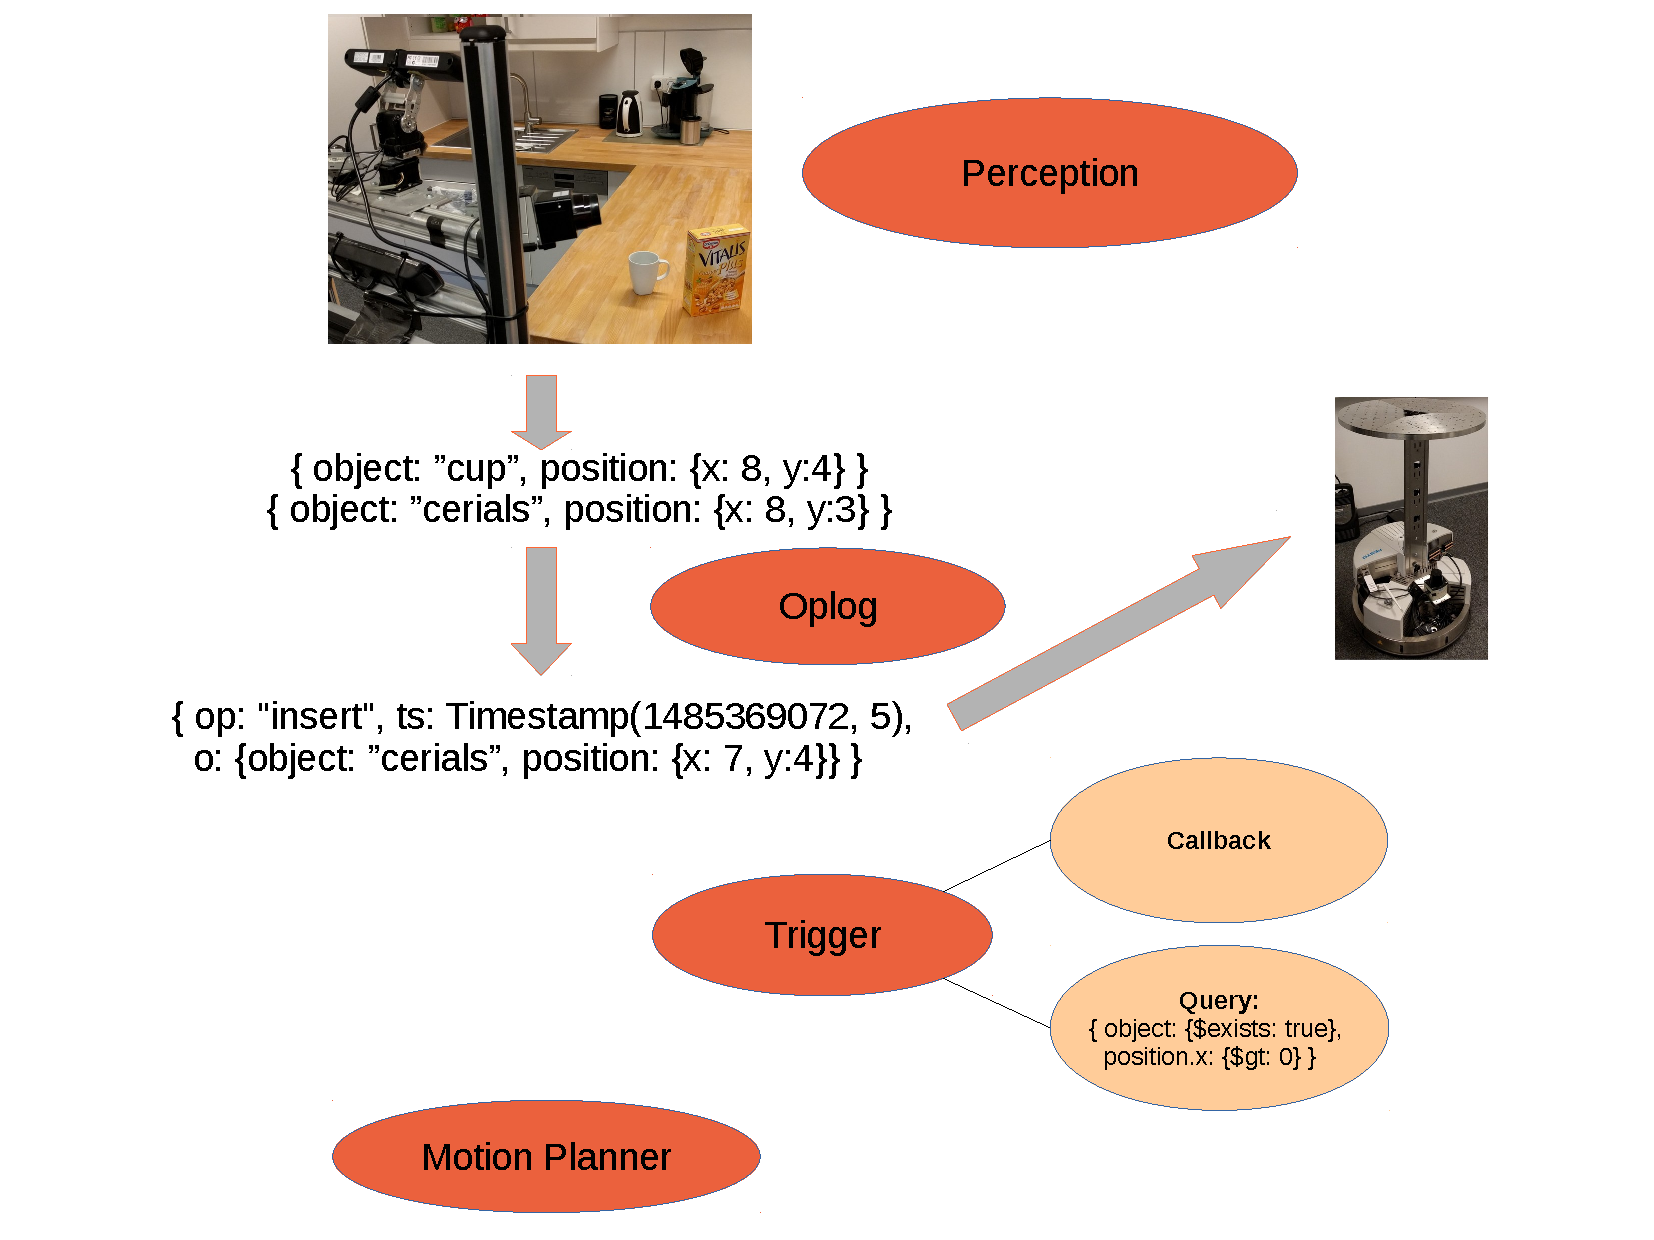
\includegraphics[width=1.03\textwidth]{../thesis/draw/trigger-1.pdf}}
  \only<6>{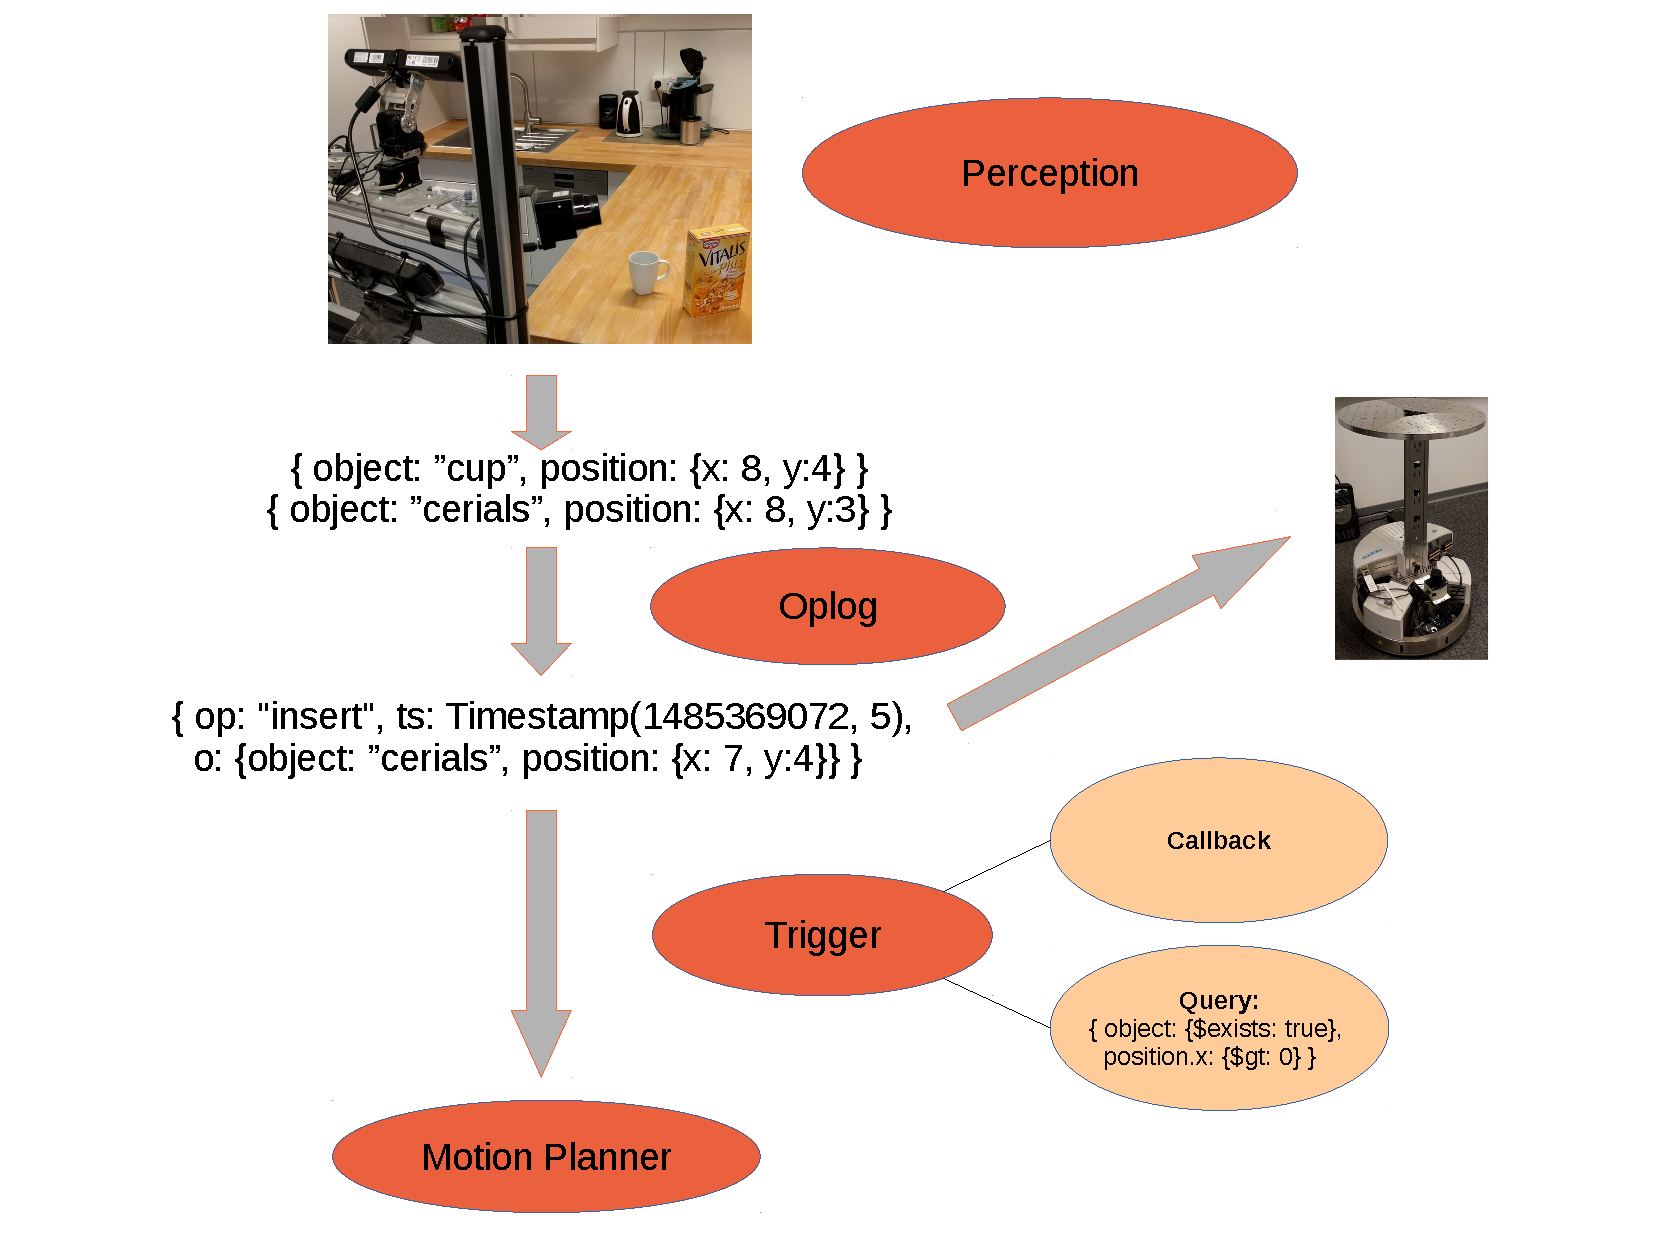
\includegraphics[width=1.03\textwidth]{../thesis/draw/trigger.pdf}}
  \pause\pause\pause\pause\pause
\end{frame}

\begin{frame}
  \frametitle{Architecture}
  \hspace{-1.3cm}
  \only<1>{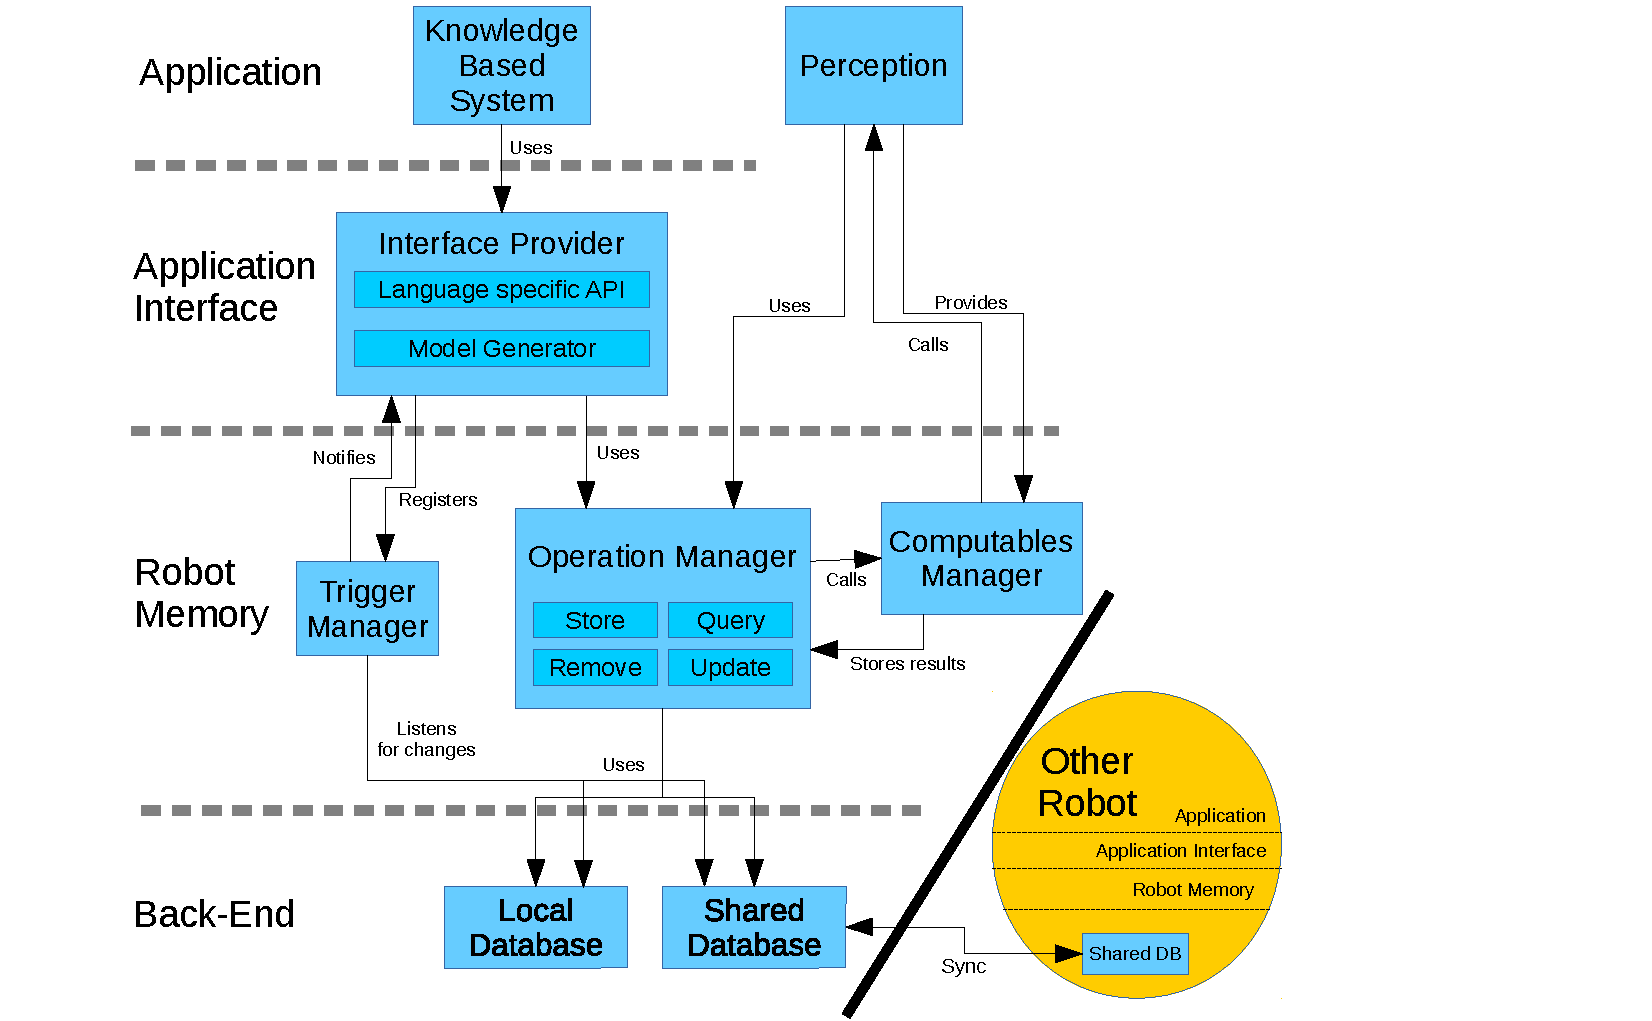
\includegraphics[width=1.1\textwidth]{../thesis/draw/architecture.pdf}}
  \only<2>{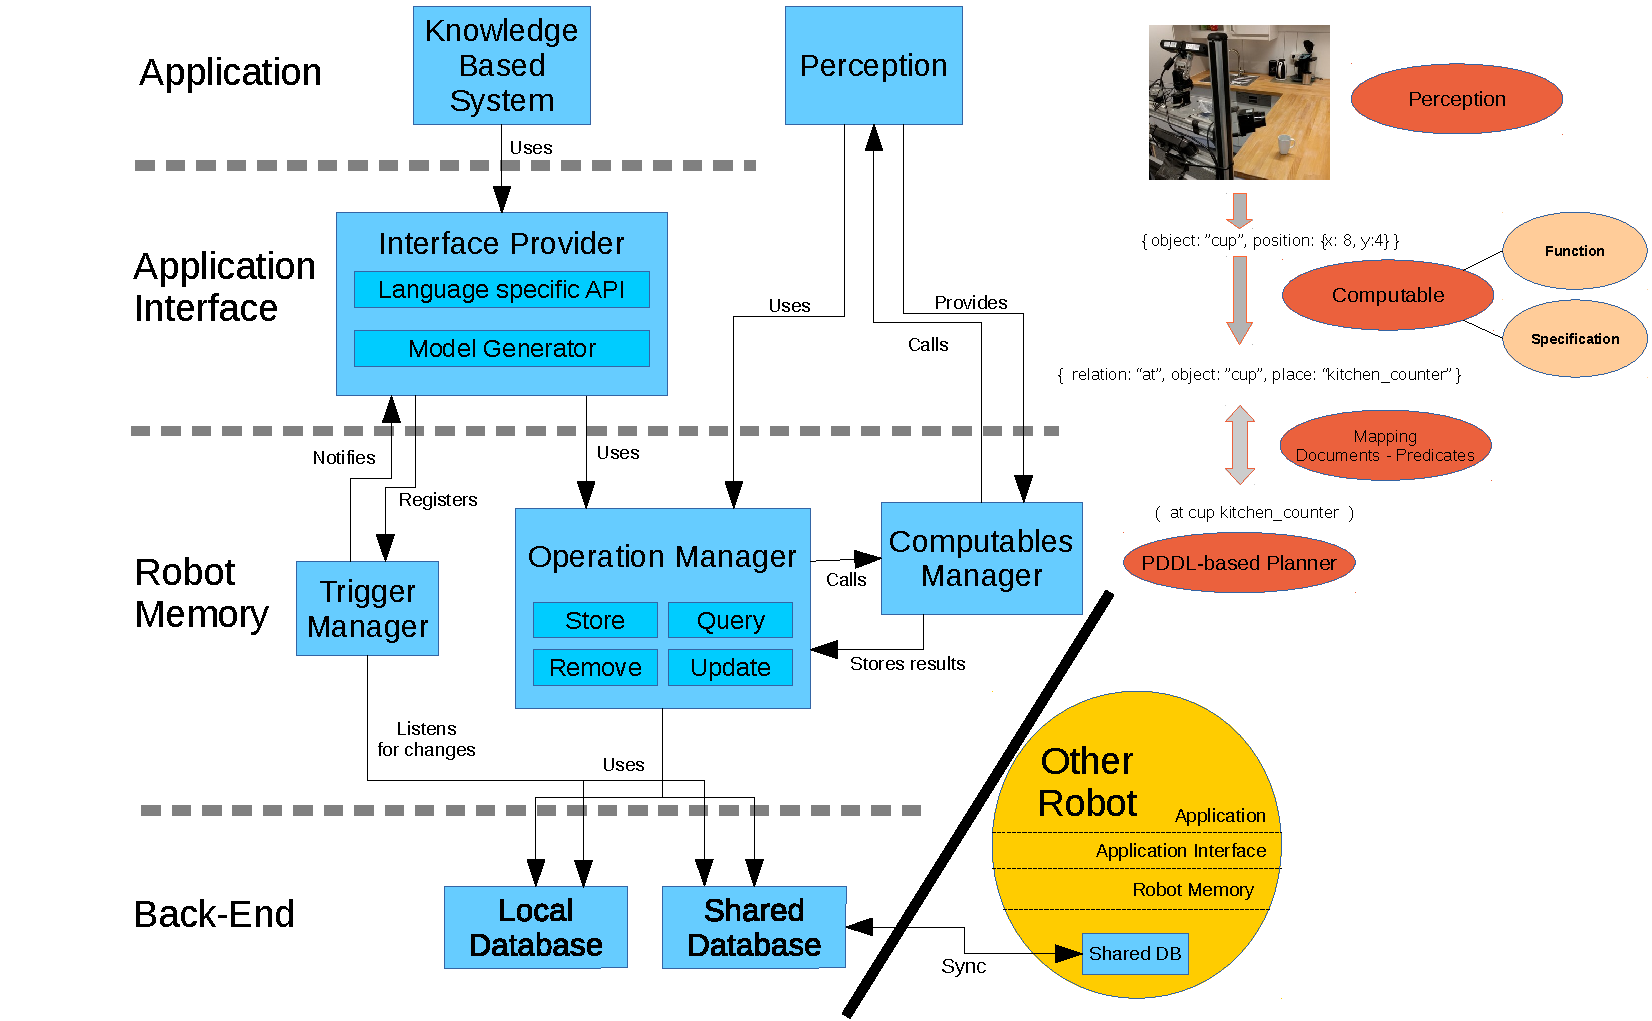
\includegraphics[width=1.1\textwidth]{../thesis/draw/architecture-comp.pdf}}
  \pause
\end{frame}


\section{Implementation}
\begin{frame}[plain]
  \tableofcontents[currentsection]
\end{frame}
\addtocounter{framenumber}{-1}

\begin{frame}
  \frametitle{Back-End and Robot Memory}
  \begin{description}
  \item[Distribution in multi-robot system]
                \hfill \\
    \begin{itemize}
    \item Write operations only on primary instance
    \item Eventual consistency on secondaries %(forwarding changes, denormalization)
    %\item No sharding because WiFi, one robot in breakdown
    \end{itemize}
\bigskip
  \item[Robot Memory]
                \hfill \\
    \begin{itemize}
    \item Modifying queries and inserts
    \item Trigger and computable managers
    \item Caching of computed documents
    \item Automated start-up of MongoDB
    \end{itemize}
  \end{description}
\end{frame}

% how to interface robot memory from planners and reasoners
% and how to map documents into specific concepts

\begin{frame}[fragile]
  \frametitle{CLIPS Interface}
  \begin{description}
  \item[CLIPS Characteristics]%<uncover@1->
                \hfill \\
    \begin{itemize}
    \item Fact base as working memory
  \begin{lstlisting}[showlines,style=ReallySmallCLIPS,
  framexleftmargin=4pt, xleftmargin=0pt,
  emph={skill, args, state, target, res},
  emphstyle=\bfseries\color{green!80!black},
  emph={[2]\?skill, \$\?args, cap-station, \?target, use,
  WAIT-FOR-LOCK, SKILL-EXECUTION, running},
  emphstyle={[2]\bfseries\color{blue!80!black}},
  morekeywords={retract, assert, modify, skill-call, skill-to-execute,
    wait-for-lock},
  numbers=none]
(cap-station (name M-CS1) (loaded NONE) (caps-on-shelf 3))
\end{lstlisting} %$ This is just to fix Emacs highlighting due to dollar sign in code above
    \item Condition-action rules
    \item Procedural functions
    \end{itemize}
  \item[Robot Memory Interface]%<uncover@2->
                \hfill \\
    \begin{itemize}
    \item Provide operation and traversal functions in CLIPS % insert, query, update, get-key, construct document
    \item Mapping between facts and documents
\begin{lstlisting}[style=SmallJSON,
  framexleftmargin=0pt, xleftmargin=0pt,
 morekeywords={}, numbers=none]
 { relation: "cap-station", name: "M-CS1",
   loaded: "NONE", caps-on-shelf: NumberLong(3)}
\end{lstlisting}
    \item Assert trigger events as facts
    \end{itemize}
  \end{description}
\end{frame}

\begin{frame}[fragile]
  \frametitle{PDDL Interface}
  \begin{description}
  \item[PDDL Characteristics]%<uncover@1->
                \hfill \\
    \begin{itemize}
    \item Domain definition and problem description as input %for PDDL-based planner
    \item Predicates represent information
\begin{lstlisting}[style=SmallSlidePDDL,
  framexleftmargin=1pt, xleftmargin=1pt,linewidth=9.5cm,
 morekeywords={}, numbers=none]
  (:goal (on A B))
  (:init (on-table A) (on-table B))
\end{lstlisting}
    \end{itemize}
  \item[Robot Memory Interface]%<uncover@2->
                \hfill \\
    \begin{itemize}
    \item Mapping of documents to predicates
    \item Generation of problem description from template
\begin{lstlisting}[style=SmallSlidePDDL,
  framexleftmargin=1pt, xleftmargin=1pt,linewidth=9.5cm,
 morekeywords={}, numbers=none]
  (:goal <<GOAL>>)
  (:init  <<#ONTABLE|{relation:'on-table'}>>
            (on-table <<object>>) <</ONTABLE>>))
\end{lstlisting}
\begin{lstlisting}[style=SmallJSON,
  framexleftmargin=0pt, xleftmargin=0pt,linewidth=9.5cm,
 morekeywords={}, numbers=none]
 { relation: "on-table", object: "A"},
 { relation: "on-table", object: "B"}
\end{lstlisting}
    \item Parses resulting plans and inserts them as documents % used Fast Forward in thesis
    \end{itemize}
  \end{description}
\end{frame}

\begin{frame}[fragile]
  \frametitle{OpenRAVE Interface}
  \begin{columns}
    \begin{column}{0.6\textwidth}
  \begin{description}
  \item[OpenRAVE Characteristics]%<uncover@1->
                \hfill \\
    \begin{itemize}
    \item Geometric motion planner
    \item Operates in continuous space
    \end{itemize}
  \item[Robot Memory Interface]%<uncover@2->
                \hfill \\
    \begin{itemize}
    \item Updates planner scene\\ based on positions\\ represented in documents
\begin{lstlisting}[style=SmallJSON,
  framexleftmargin=5pt, xleftmargin=0pt,linewidth=5cm,
 morekeywords={}, numbers=none]
{
  block: "B",
  frame: "map",
  translation:
    [0.43, -0.04, 0.01]
}
\end{lstlisting}
    %\item Configurable models and queries
    \end{itemize}
  \end{description}
    \end{column}
    \begin{column}{0.4\textwidth}
    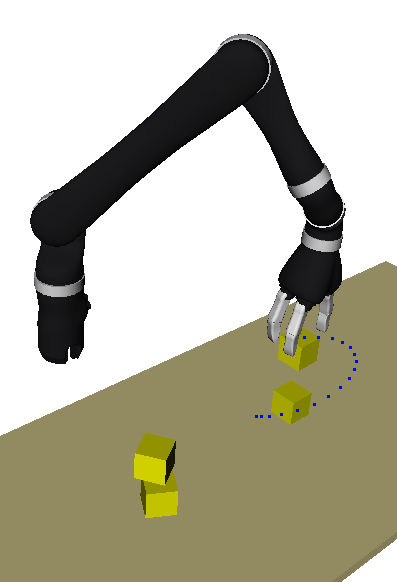
\includegraphics[width=\textwidth]{../thesis/img/openrave-blocks}
    \end{column}
  \end{columns}
\end{frame}

\begin{frame}
  \frametitle{Application and evaluation scenarios}
  \begin{columns}
    \begin{column}{0.5\textwidth}
    \textbf{World model synchronization between robots in the RCLL}\\
    \vspace{0.6cm}
    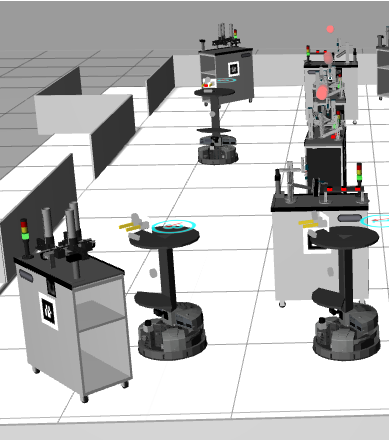
\includegraphics[width=0.9\textwidth]{../thesis/img/rcll-sim-slim}
%% share knowledge to collaborate
    \end{column}
    \begin{column}{0.4\textwidth}
    \textbf{Blocks world with a robot arm}\\
    \vspace{0.6cm}
    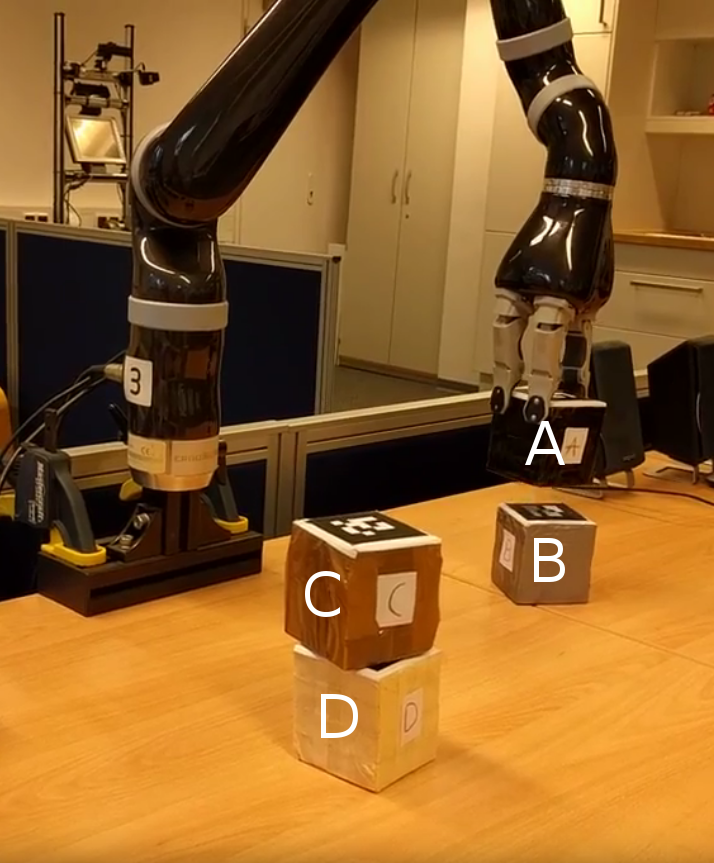
\includegraphics[width=\textwidth]{../thesis/img/blocks-world-annotated}
    \end{column}
  \end{columns}
\end{frame}


\section{Evaluation}
\begin{frame}[plain]
  \tableofcontents[currentsection]
\end{frame}
\addtocounter{framenumber}{-1}

\begin{frame}
  \frametitle{Qualitative Evaluation}
  \begin{description}
  \item[Experience from evaluation scenarios]%<uncover@1->
                \hfill \\
    \begin{itemize}
    \item Flexible storage and expressive querying
    \item Convenient memory sharing between KBS\\ and in distributed system
    % \item Planner specific views on a common\\ and thus consistent information basis
      % (geometric for motion planner, symbolic for pddl)
    \item Allows hybrid reasoning with computables\\(e.g. \texttt{on-table} derived from geometric position)
      % Transformation of geometric block position to on-table predicate
    \item Triggers useful for worldmodel updates and messages
    \end{itemize}
  \end{description}
\begin{block}{}%<uncover@2->
  \begin{itemize}
  \item Beneficial for AI/robot software development
  \item Especially for combining different planners/reasoners
  \end{itemize}
  \end{block}
\end{frame}

\begin{frame}
  \frametitle{Qualitative Evaluation: Limitations}
  \begin{description}
  \item[Trade-offs / Limitations]
                \hfill \\
\bigskip
    \begin{itemize}
    \item Trigger only for changes of single documents % (ok because of denormalization)
\vspace{0.15cm}
    \item No direct trigger evaluation for computables % mention complexity, posisble with workaround
\vspace{0.15cm}
    \item Query complexity determined by application % formulation important
    \end{itemize}
  \end{description}
\end{frame}

\begin{frame}[fragile]
  \frametitle{Quantitative Evaluation}
  \begin{columns}
    \begin{column}{0.55\textwidth}
      \begin{description}
      \item[Tidy up scenario] \hfill \\
        \begin{itemize}
        \item Robot Memory with information about objects
          \begin{lstlisting}[style=SmallJSON,
            framexleftmargin=5pt, xleftmargin=0pt,
            morekeywords={}, numbers=none]
{ name: "coffee machine",
  position: "counter",
  tidied: "counter" },
{ name: "milk",
  position: "counter",
  tidied: "fridge" }
          \end{lstlisting}
        \item Measure operation durations with increasing domain size
        \item With / without indexing
        \end{itemize}
      \end{description}
    \end{column}
    \begin{column}{0.45\textwidth}
      \centering
    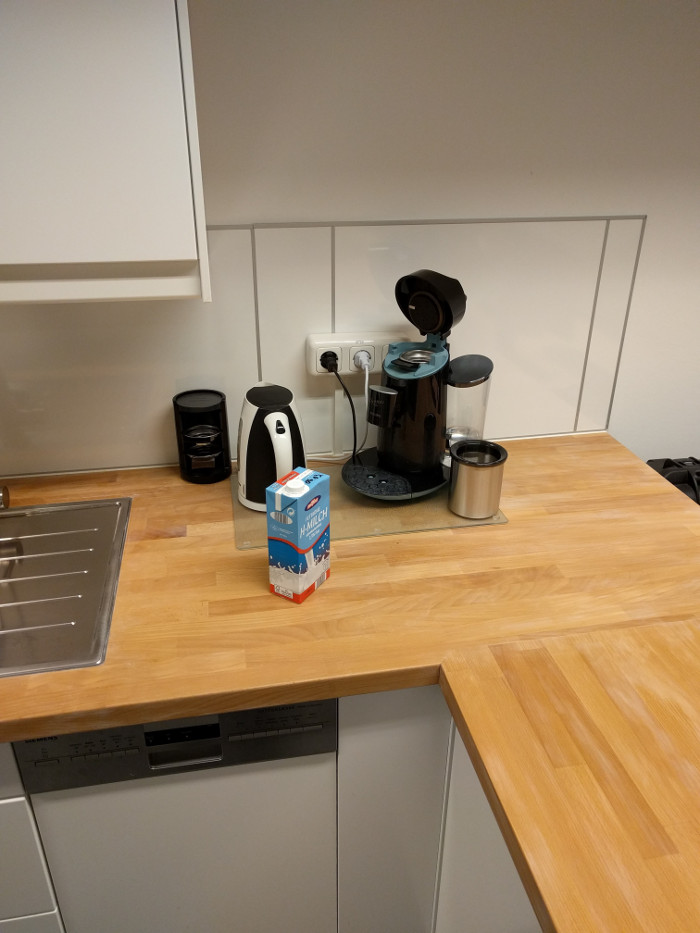
\includegraphics[width=0.9\textwidth]{../thesis/img/tidy-up}\\
    \end{column}
  \end{columns}
\end{frame}

\begin{frame}
  \frametitle{Duration of Robot Memory Operations I}
  \centering
  \begin{columns}
    \begin{column}{0.55\textwidth}
  \centering
    \small
    \\\vspace{-0.15cm}
    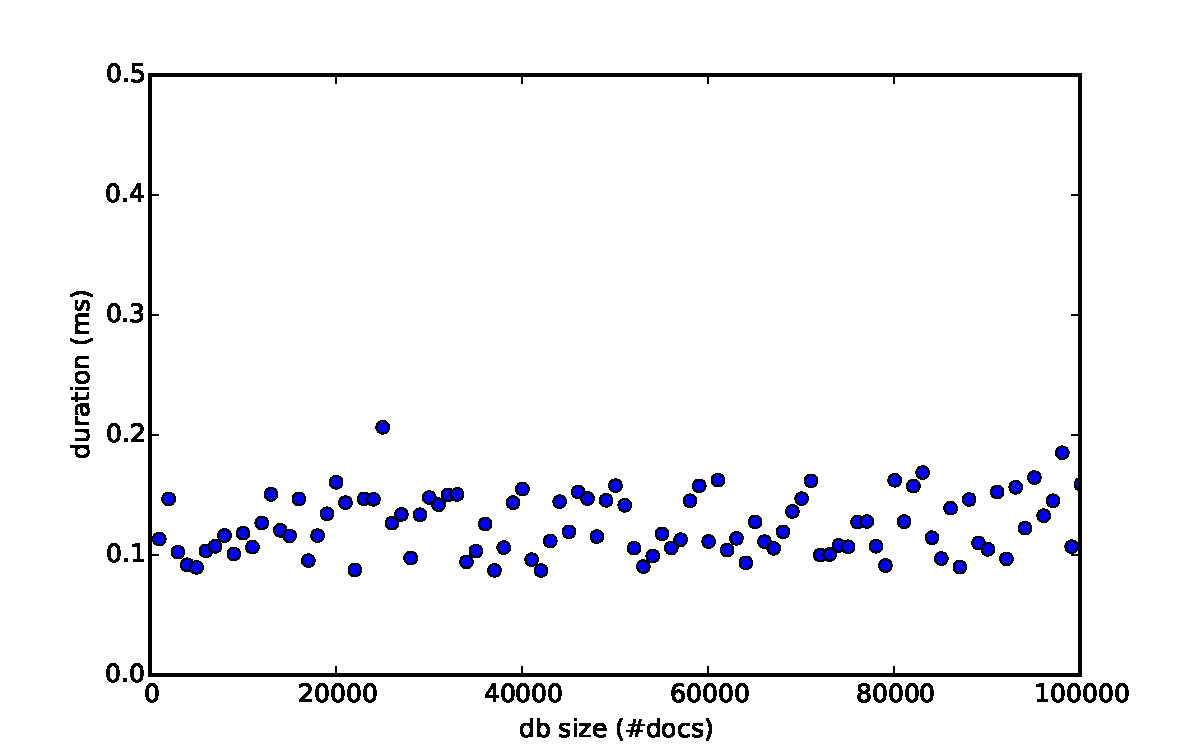
\includegraphics[width=\textwidth]{../thesis/plots/insert-durations}\\
    \\\vspace{-0.05cm}
    Insertions
    \\\vspace{-0.05cm}
    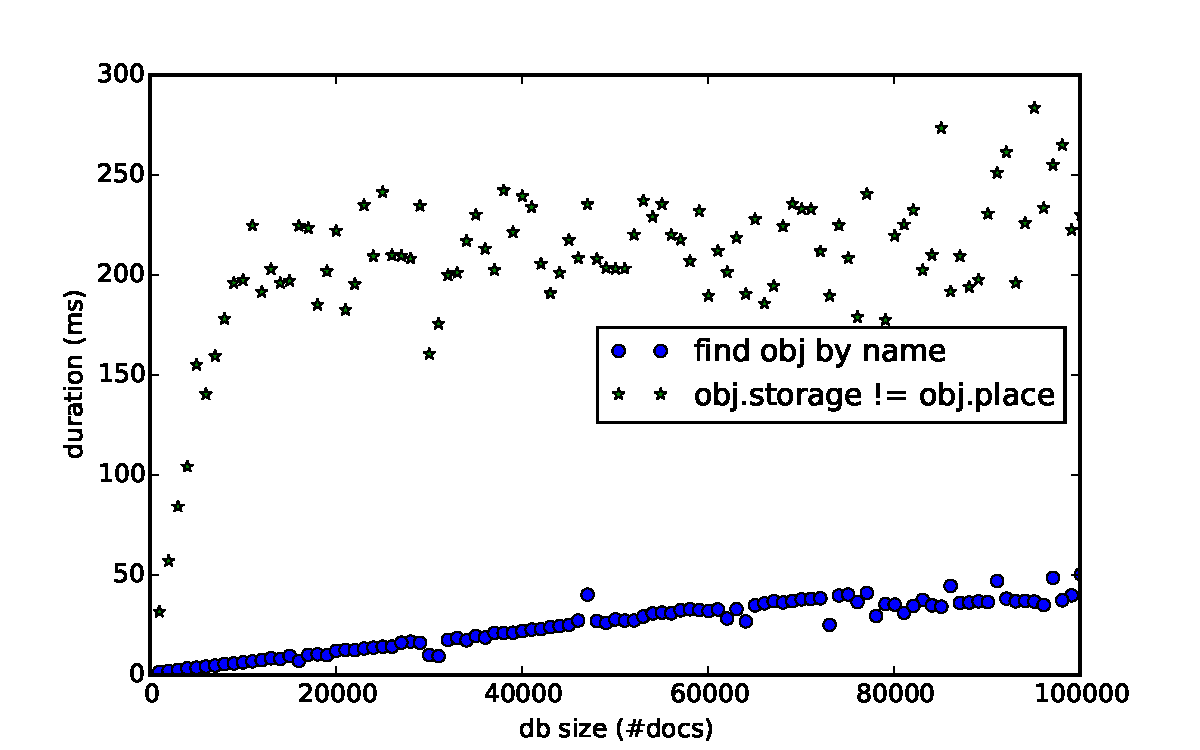
\includegraphics[width=\textwidth]{../thesis/plots/query-durations}\\
    \\\vspace{-0.08cm}
    Queries
    \end{column}
    \begin{column}{0.55\textwidth}
  \centering
    \small
    \\\vspace{-0.15cm}
    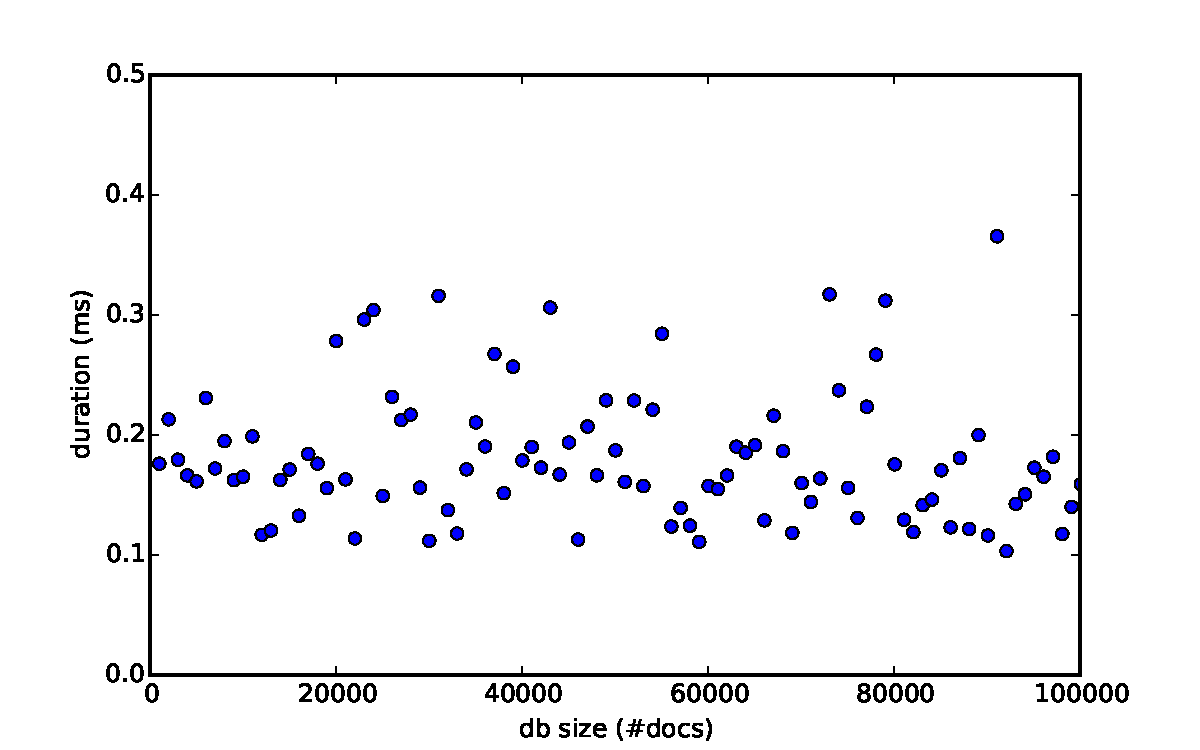
\includegraphics[width=\textwidth]{../thesis/plots/insert-durations-index}\\
    \\\vspace{-0.05cm}
    Insertions with Indexing
    \\\vspace{-0.08cm}
    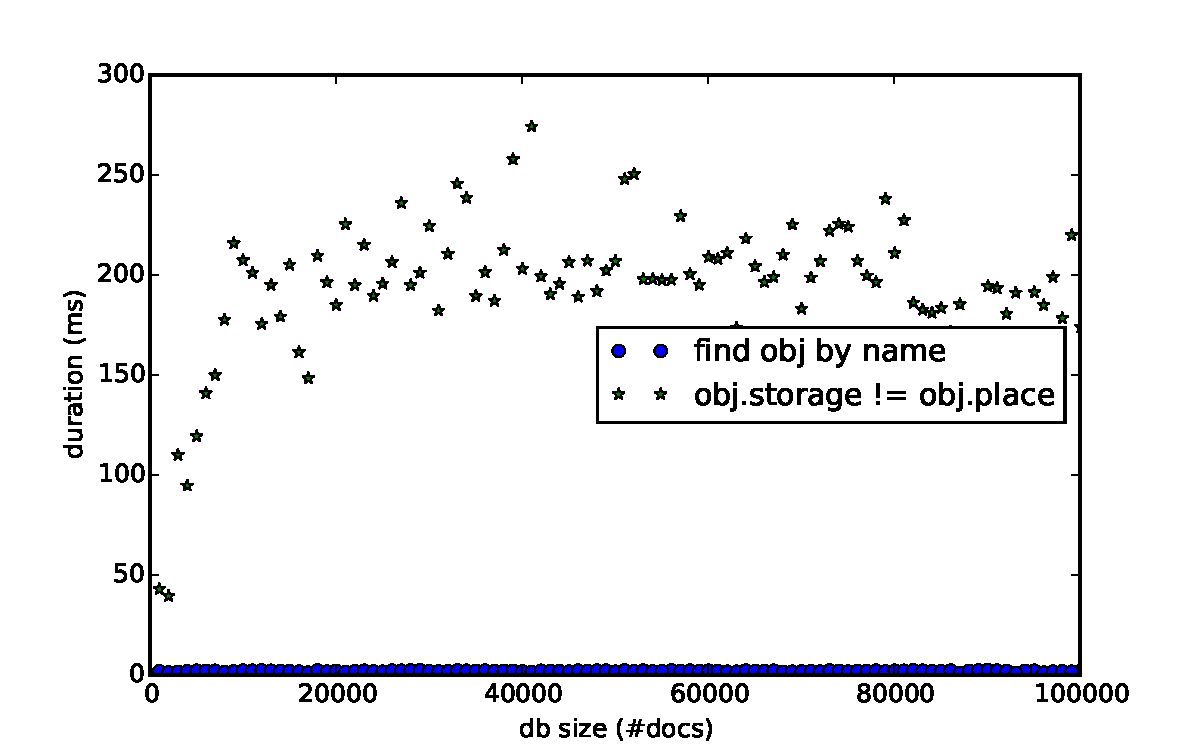
\includegraphics[width=\textwidth]{../thesis/plots/query-durations-index}\\
    \\\vspace{-0.05cm}
    Queries with Indexing
    \end{column}
  \end{columns}
\end{frame}

\begin{frame}
  \frametitle{Duration of Robot Memory Operations II}
  \centering
  \begin{columns}
    \begin{column}{0.55\textwidth}
  \centering
    \small
    \\\vspace{-0.17cm}
    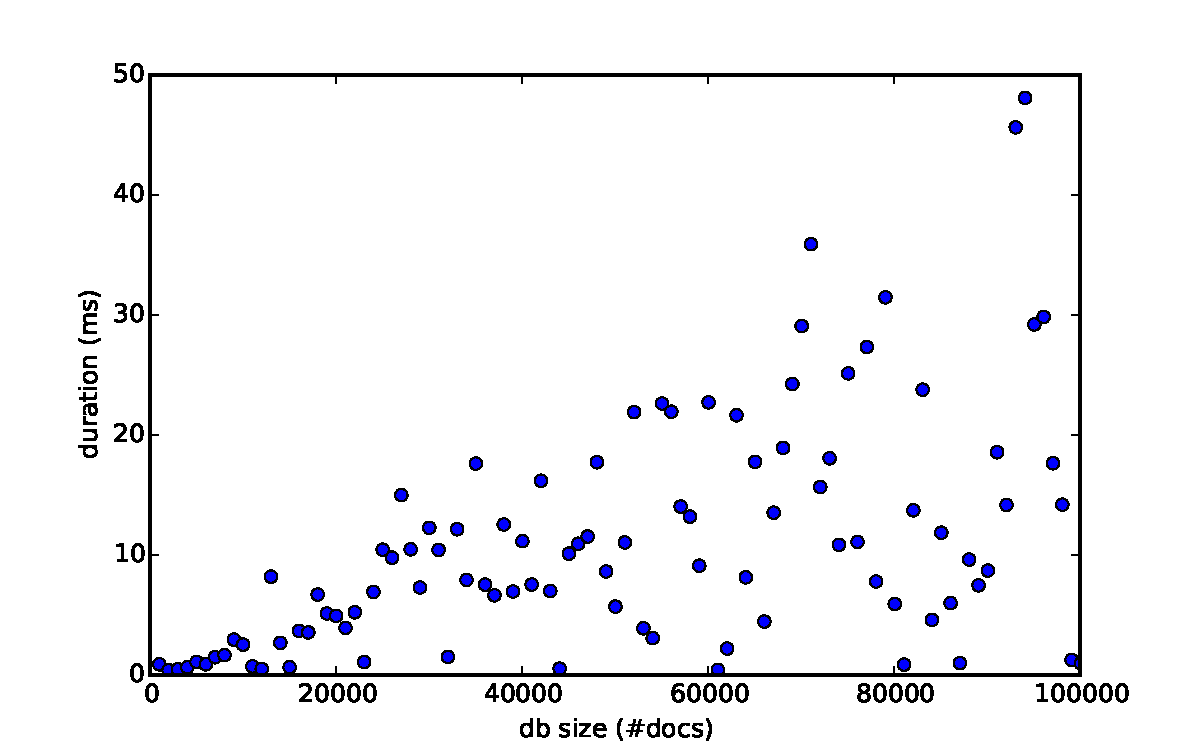
\includegraphics[width=\textwidth]{../thesis/plots/update-durations}\\
    \\\vspace{-0.08cm}
    Updates
    \\\vspace{-0.05cm}
    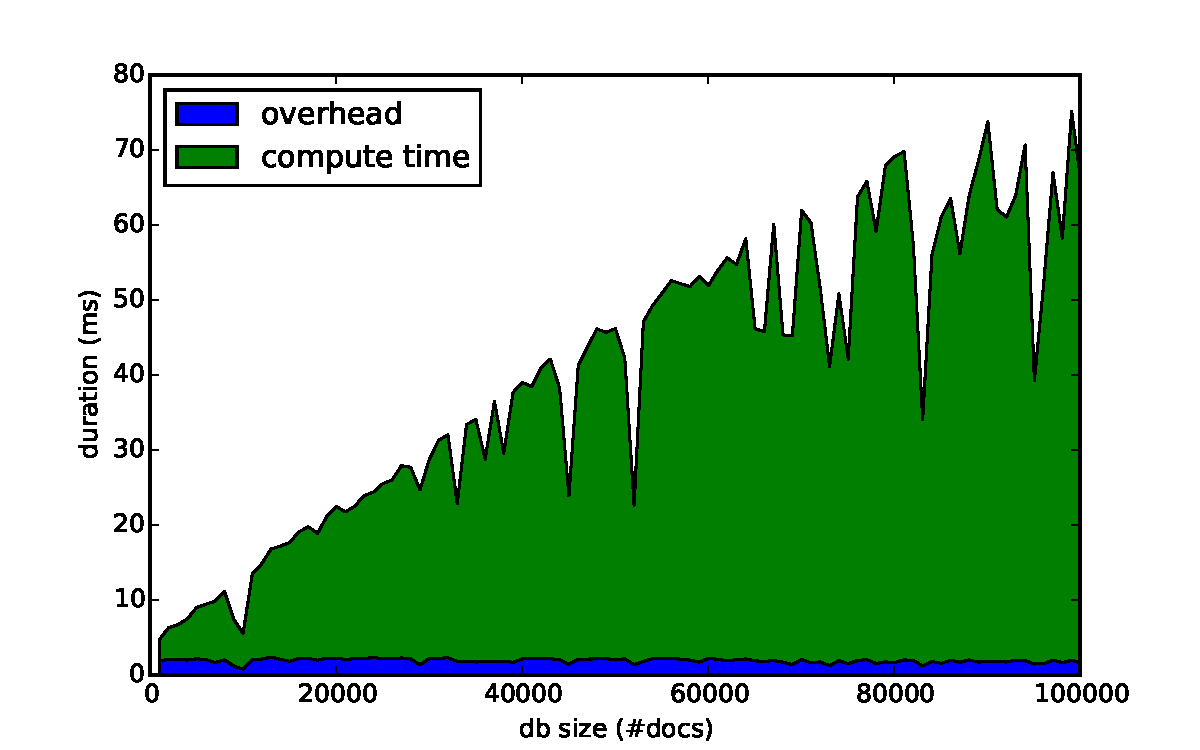
\includegraphics[width=\textwidth]{../thesis/plots/computable-durations}\\
    \\\vspace{-0.05cm}
    Computables
    \end{column}
    \begin{column}{0.55\textwidth}
  \centering
    \small
    \\\vspace{-0.17cm}
    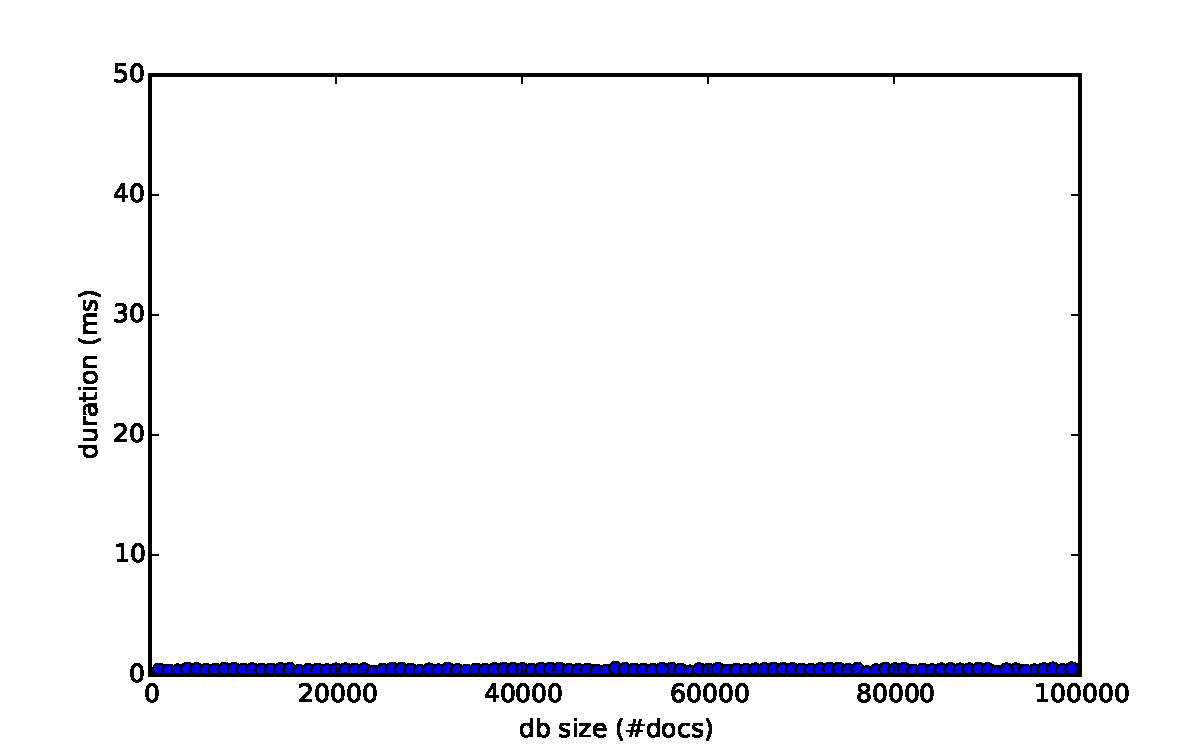
\includegraphics[width=\textwidth]{../thesis/plots/update-durations-index}\\
    \\\vspace{-0.08cm}
    Updates with Indexes
    \\\vspace{-0.05cm}
    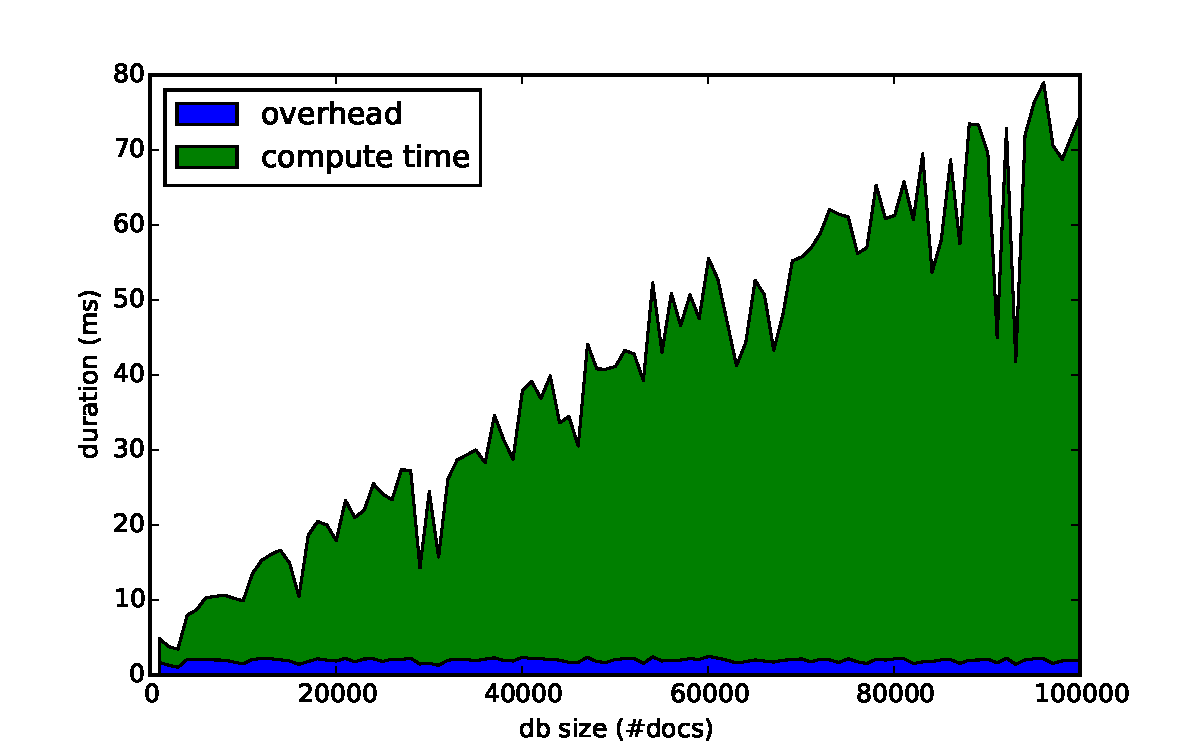
\includegraphics[width=\textwidth]{../thesis/plots/computable-durations-index}\\
    \\\vspace{-0.05cm}
    Computables with Indexes
    \end{column}
  \end{columns}
\end{frame}


\section{Conclusion}
\begin{frame}[plain]
  \tableofcontents[currentsection]
\end{frame}
\addtocounter{framenumber}{-1}

\begin{frame}
  \frametitle{Foundation for Future Projects}
  \begin{description}
  \item[Two projects currently using the Robot Memory]\hfill\\
    \begin{itemize}
    \item Both for centralized global task planning in the RCLL
    \item Reactive ASP and real-time constraints
    \item PDDL with temporal aspects
    \end{itemize}
  \item[Beneficial features] \hfill \\
    \begin{itemize}
    \item Distributed memory shared by planner and executives
    \item CLIPS agent integration
    \item Triggers for notifications
    \item PDDL problem definition generation
    \end{itemize}
  \end{description}
\end{frame}

\begin{frame}
  \frametitle{Conclusion and Questions}
  \begin{block}{Generic Robot Memory } \centering\bfseries
    flexible storage and expressive querying for hybrid reasoning and world model sharing between different KBS
  \end{block}
  \bigskip
  \begin{columns}
    \begin{column}{0.5\textwidth}
      \begin{itemize}
      \item Document-oriented representation and querying
      \item Distributable and persistent
      \item Theoretical foundation
      \item Triggers for notification
      % \item Architectural design
      % \item Interfaces for KBS
      %\item Hybrid reasoning with computables
      \end{itemize}
    \end{column}
    \begin{column}{0.5\textwidth}
      \begin{itemize}
      \item Computables
      \item Symbolic/spatio-temporal
      \item Beneficial and efficient in application scenarios
      \item Foundation for future projects
      \end{itemize}
    \end{column}
  \end{columns}
\end{frame}



%%%%%%%%%%%%%%%%%%%%%%%%%%%%%%%%%%%%%%%%%%%%%%%%%%%%%%%%%%%%%%%%%%%%%%%%%%%%%%%%%%%%%%%%%%%%%%%%%%%%
%%%%%%%%%%%%%%%%%%%%%%%%%%%%%%%%%%%%%%%%%%%%%%%%%%%%%%%%%%%%%%%%%%%%%%%%%%%%%%%%%%%%%%%%%%%%%%%%%%%%
%%%%%%%%%%%%%%%%%%%%%%%%%%%%%%%%%%%%%%%%%%%%%%%%%%%%%%%%%%%%%%%%%%%%%%%%%%%%%%%%%%%%%%%%%%%%%%%%%%%%

\newcounter{finalframe}
\setcounter{finalframe}{\value{framenumber}}


\begin{frame}[allowframebreaks]
  \frametitle{References}
  \small
  \bibliographystyle{apalike}
  \bibliography{../references}
\end{frame}

% Backup Slides

\begin{frame}
  \frametitle{Theoretical Foundation}
\begin{description}[]
  \item[Definition of documents representing knowledge] \hfill \\
  \small e.g.~$\{("object","cup"),("room","kitchen"),("position",{\scriptstyle\{("x",8),("y",4)\}})\}$
  \begin{enumerate}
\item \textbf{Keys:} $\mathcal{K} := \Sigma^*$
\item  \textbf{Atomic values:} $\mathcal{V}_0$ are constants
\item \textbf{Unnested key-value pairs:} $\mathcal{P}_0:=\mathcal{K}\times\mathcal{V}_0$
\item \textbf{Unnested documents:} \vspace{-0.3cm}
%are sets of key-value pairs with unique keys and thus included in the power set of $\mathcal{P}_0$:\\
\begin{align*}
\mathcal{D}_0:=\{
  d\in\mathbb{P}(\mathcal{P}_0)|
  \forall (k,v),(k',v')\in d , k\neq k' \vee (k,v)=(k',v')
  \}
\end{align*}
\end{enumerate}
  \item[With nesting] \hfill \\
  \begin{enumerate}
\item  \textbf{Values:} $\mathcal{V}_n := \mathcal{V}_{n-1} \cup \mathcal{D}_{n-1}$
\item \textbf{Key-Value Pairs:} $\mathcal{P}_n:=\mathcal{K}\times\mathcal{V}_n$
\item \textbf{Documents:} \vspace{-0.3cm}
\begin{align*}
  \mathcal{D}_n:=\{
  d\in\mathbb{P}(\mathcal{P}_n)|
  \forall (k,v),(k',v')\in d , k\neq k' \vee (k,v)=(k',v')
  \}
\end{align*}
\end{enumerate}
  \end{description}
  \textbf{Finitely nested documents:} $\mathcal{D}=\cup_{n\in\mathbb{N}}\mathcal{D}_n$\\
  \textbf{Values:} $\mathcal{V}=\cup_{n\in\mathbb{N}}\mathcal{V}_n$
\end{frame}

\begin{frame}
  \frametitle{Theoretical Foundation}
  \begin{description}[]
  \item[Definition Robot Memory] \hfill \\
    \begin{enumerate}
      \item \textbf{Database:} finite set $\mathcal{DB} \subset \mathcal{D}$
      \item \textbf{Query:} represented by document $q\in\mathcal{D}$\\
      yields set of documents $r\subset\mathcal{DB}$ as result\\
      e.g. $q=\{("object","cup"),("room","kitchen")\}$
      \item \textbf{Computable:} $f: \mathcal{D} \rightarrow \mathbb{P}(\mathcal{D})$
      % providing computable knowledge on demand
      %computability and termination ensured by providing component
      \item \textbf{Set of Computables:} $\mathcal{C}$
      \item \textbf{Robot Memory:} $\mathcal{RM}=(\mathcal{DB},\mathcal{C})$
      \item \textbf{Memorized Documents:} $mem(\mathcal{RM})=\mathcal{DB} \cup \bigcup_{f\in\mathcal{C}}f(\mathcal{D})$
    \end{enumerate}
  \end{description}  
\end{frame}

\begin{frame}
  \frametitle{Theoretical Foundation}
    \begin{description}[]
  \item[Mapping into PDDL] \hfill \\
\vspace{-0.5cm}
\small\begin{align*}
\text{e.g. } map_p&(\{("predicate", "at"),("object", "cup"),("room","kitchen")\})\\
             &= at(map_f("cup"), map_f("kitchen")) = at(cup, kitchen) \text{.}
\end{align*}
  \begin{enumerate}
      \item \textbf{Predicate symbols} $\mathcal{R}$, \textbf{Function symbols} $\mathcal{F}$
      \item \textbf{Name mapping:}
      \begin{align*}
        name_{pred}: \mathcal{R} \rightarrow \Sigma^* &\text{ and } name_{func}: \mathcal{F} \rightarrow \Sigma^*\\
        %injective, disjunct
        name_{pred-atr}: \mathcal{R} \times \mathbb{N} \rightarrow \mathcal{K} &\text{ and } name_{func-atr}: \mathcal{F} \times \mathbb{N} \rightarrow
\mathcal{K}
      \end{align*}
      \only<1>{
      \item \textbf{Map to predicate:}
      \begin{align*}
        map_p(d)=&\text{ }p(map_f(v_1), ..., map_f(v_n)), \text{ iff } p \text{ is a n-array predicate in } \mathcal{R},\\
  ("predica&te", name_{pred}(p))\in d, \forall i \in \{1..n\} (name_{pred-atr}(p,i), v_i)\in d\\
  map_p(d)=& \text{ }nil_p, otherwise
      \end{align*}}
      \only<2>{
      \item \textbf{Map to predicate}
      \item \textbf{Map to function term:}
      \begin{align*}
        map_f(v)= &\text{ }v, v \in \mathcal{V}_0\\
        map_f(d)= &\text{ }f(map_f(v_1), ..., map_f(v_n)), \text{ iff } f \text{ is a n-array function in } \mathcal{F},\\
  ("functio&n", name_{func}(f))\in d, \forall i \in \{1..n\} (name_{func-atr}(f,i), v_i)\in d\\
  map_f(d)= &\text{ } nil_f, otherwise
      \end{align*}}
    \end{enumerate}
  \end{description}
\end{frame}
\begin{frame}[fragile]
  \frametitle{Trigger/Oplog document}
\begin{lstlisting}[style=SmallJSON,
  label=lst:Oplog,
  framexleftmargin=2pt, xleftmargin=0pt,
 morekeywords={}, numbers=none]
{
  ns: "syncedrobmem.clipswm",
  ts: Timestamp(1485369072, 5),
  op: "i",
  o: {
    _id : ObjectId("58c14a14"),
    relation: "order",
    id: 2,
    complexity: "C0",
    delivery-gate: 3,
    quantity-requested: 1,
    quantity-delivered: 0,
    begin: 209,
    end: 282 }
}
\end{lstlisting}
\end{frame}


\begin{frame}
  \frametitle{Evaluation: Duration without Indexing}
  \centering
  \begin{columns}
    \begin{column}{0.55\textwidth}
  \centering
    \small
    \\\vspace{-0.15cm}
    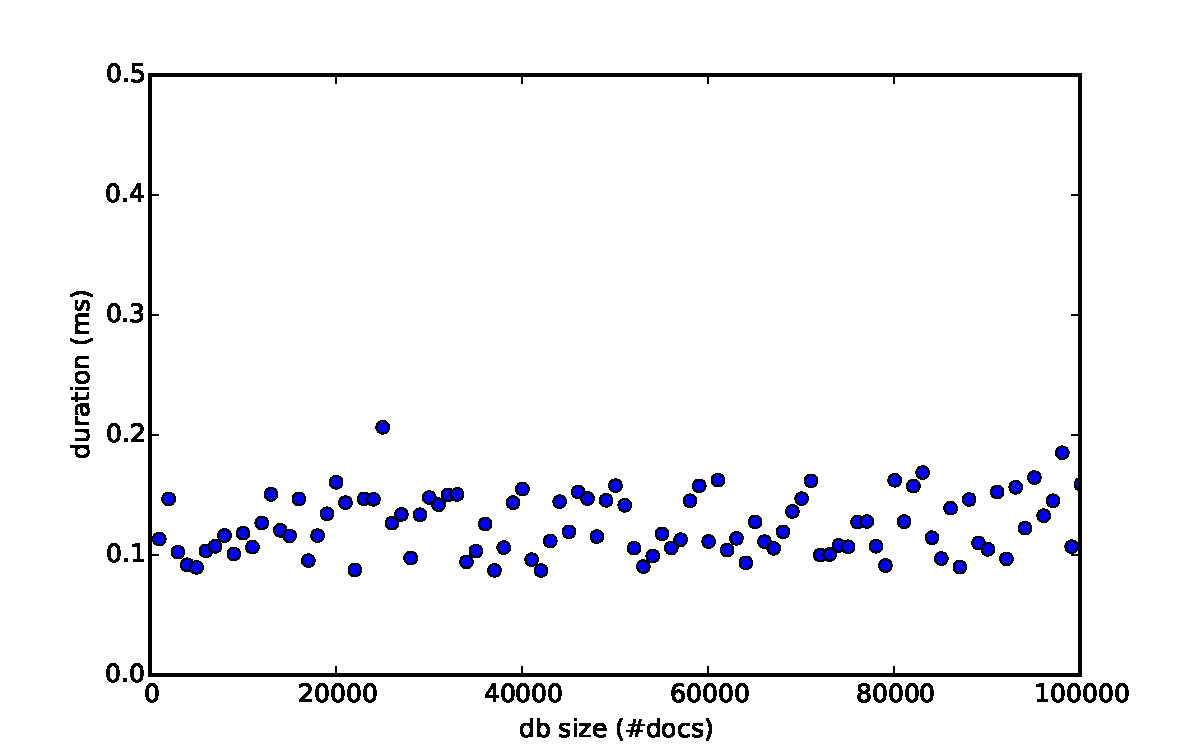
\includegraphics[width=\textwidth]{../thesis/plots/insert-durations}\\
    \\\vspace{-0.05cm}
    (a) Insertions
    \\\vspace{-0.1cm}
    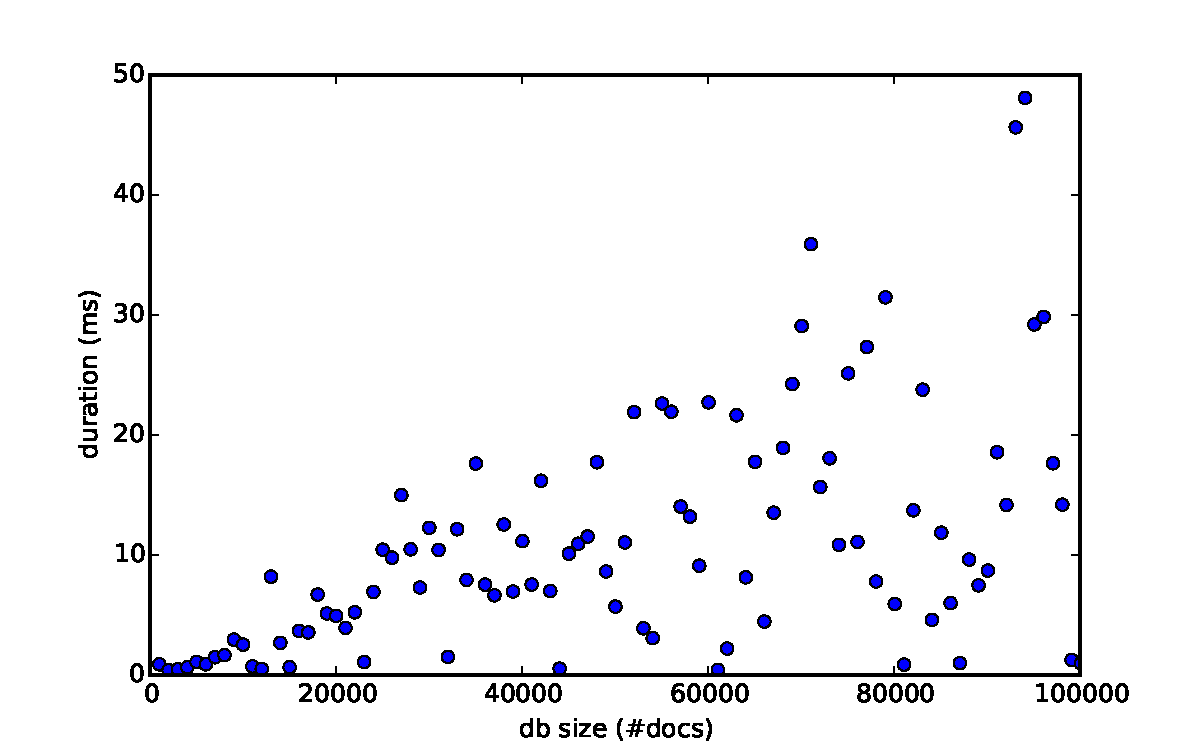
\includegraphics[width=\textwidth]{../thesis/plots/update-durations}\\
    \\\vspace{-0.05cm}
    (c) Updates
    \end{column}
    \begin{column}{0.55\textwidth}
  \centering
    \small
    \\\vspace{-0.15cm}
    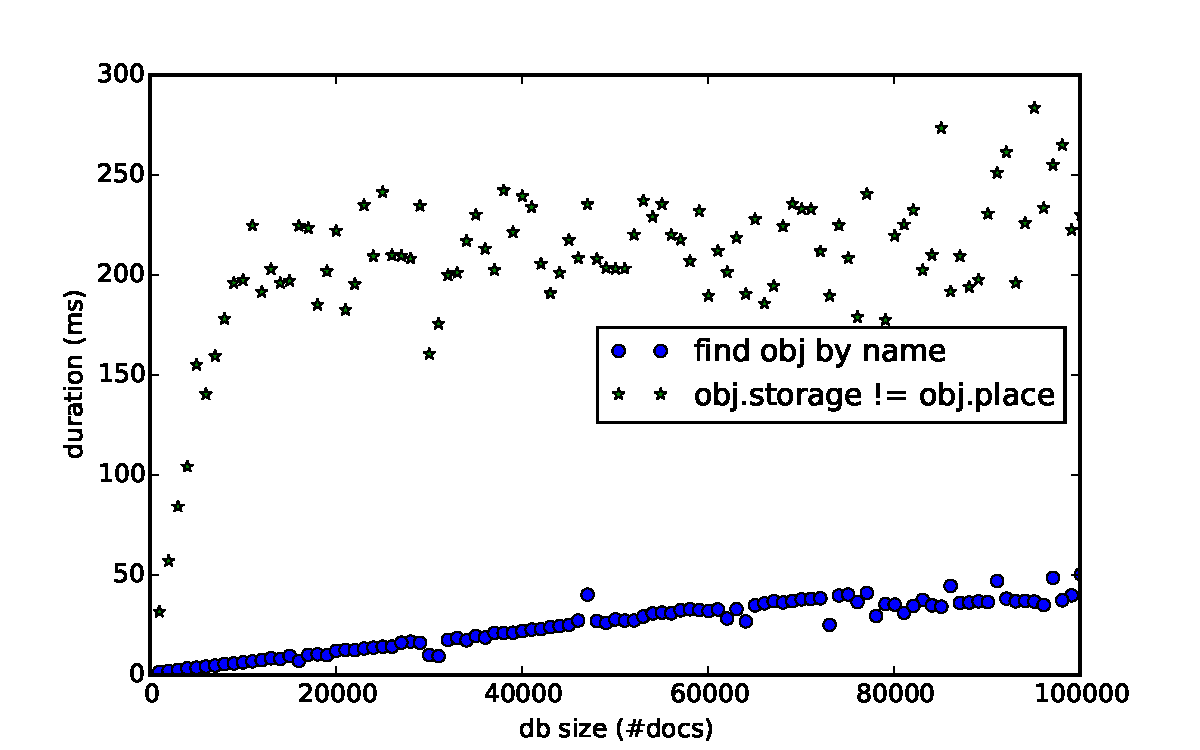
\includegraphics[width=\textwidth]{../thesis/plots/query-durations}\\
    \\\vspace{-0.05cm}
    (b) Queries
    \\\vspace{-0.1cm}
    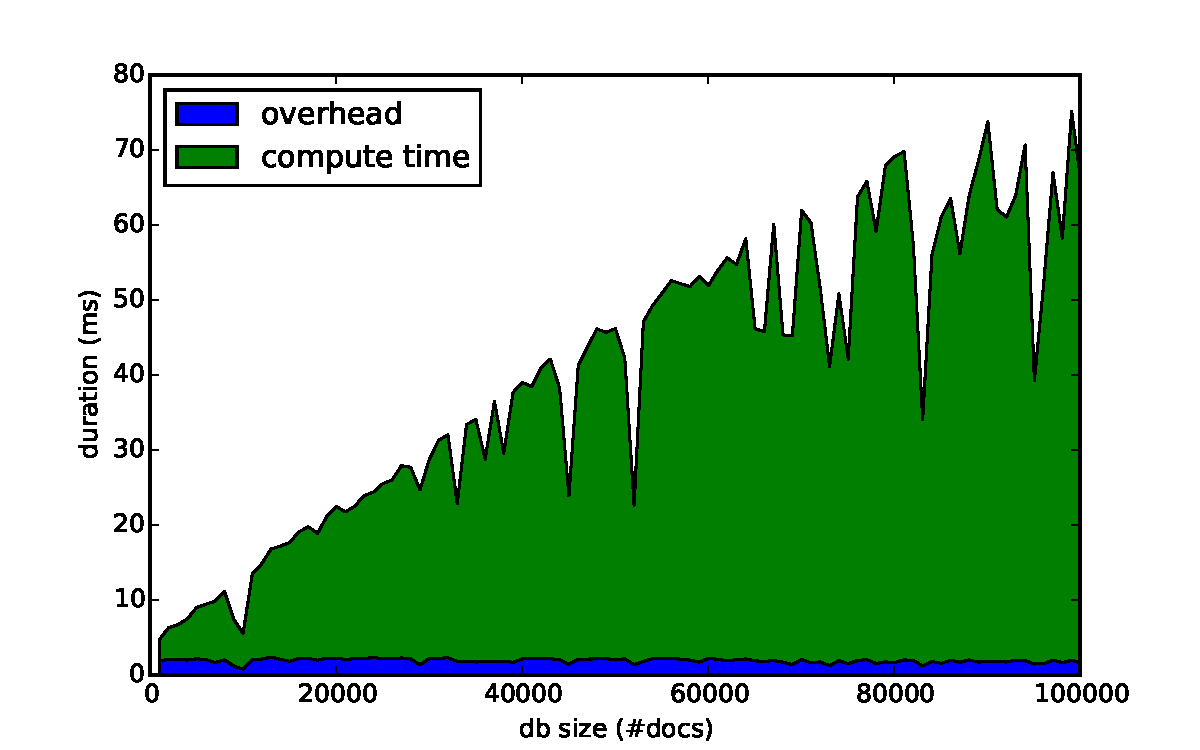
\includegraphics[width=\textwidth]{../thesis/plots/computable-durations}\\
    \\\vspace{-0.05cm}
    (d) Computables
    \end{column}
  \end{columns}
\end{frame}

\begin{frame}
  \frametitle{Evaluation: Durations with Indexing}
  \centering
  \begin{columns}
    \begin{column}{0.55\textwidth}
  \centering
    \small
    \\\vspace{-0.15cm}
    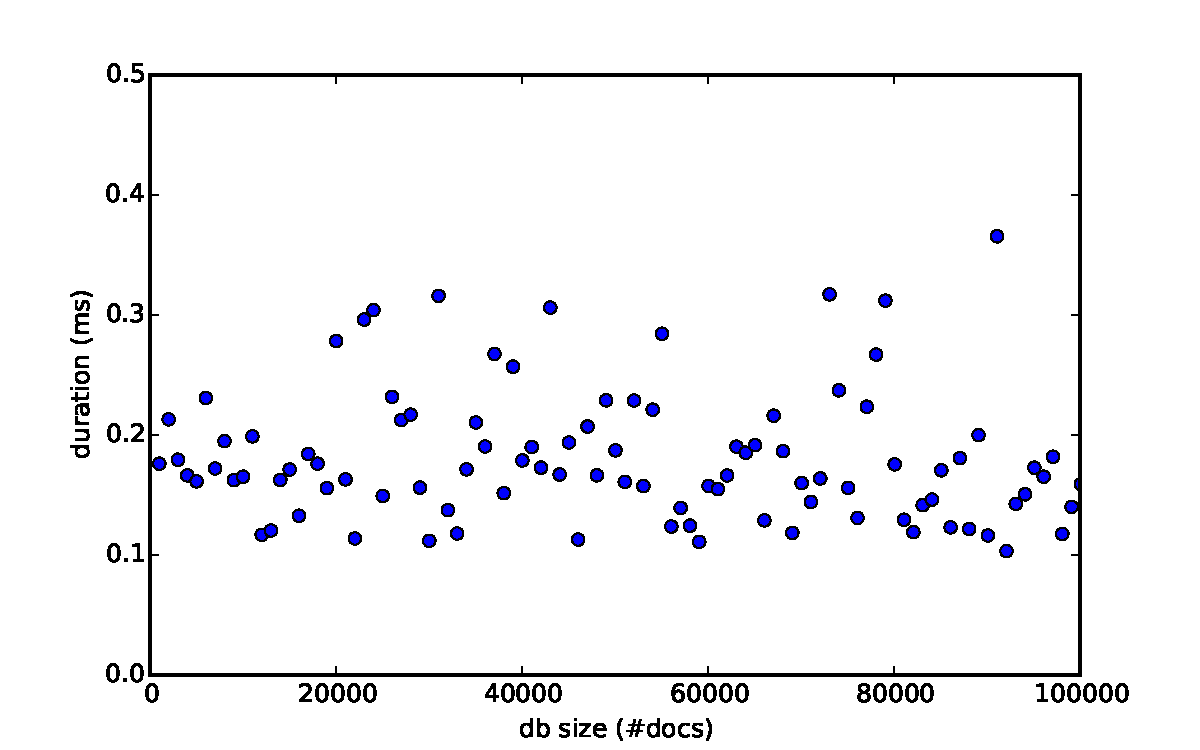
\includegraphics[width=\textwidth]{../thesis/plots/insert-durations-index}\\
    \\\vspace{-0.05cm}
    (a) Insertions
    \\\vspace{-0.1cm}
    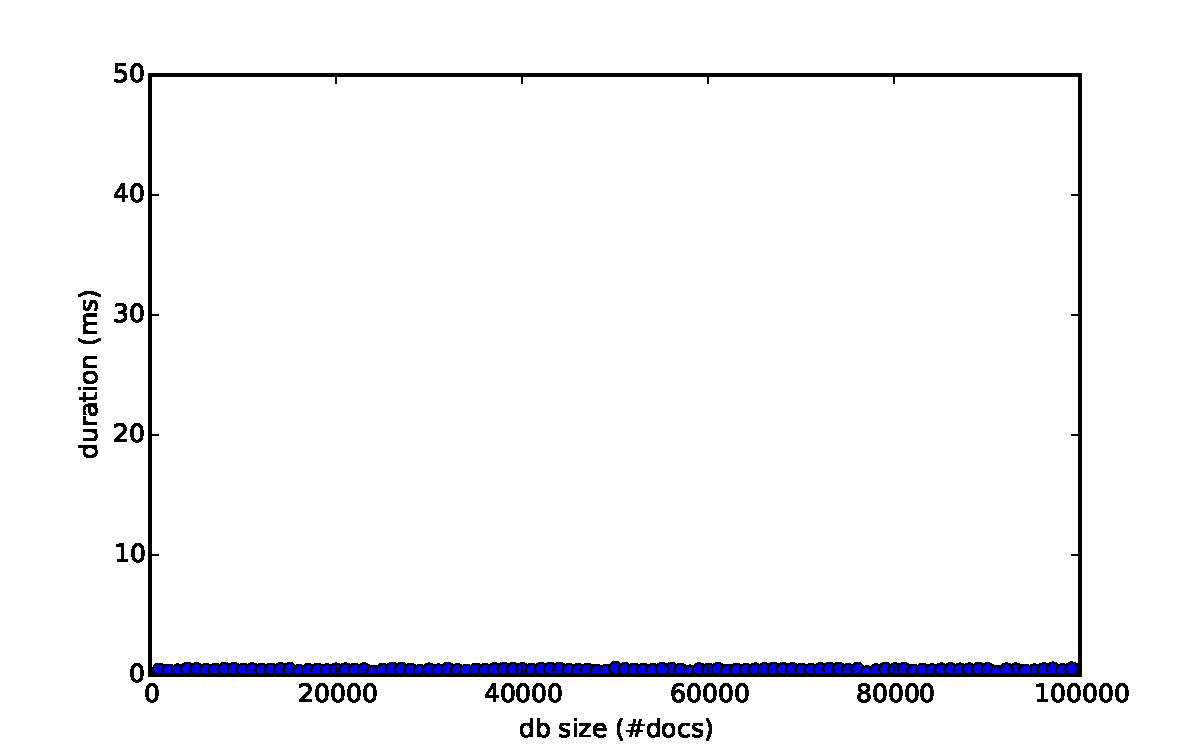
\includegraphics[width=\textwidth]{../thesis/plots/update-durations-index}\\
    \\\vspace{-0.05cm}
    (c) Updates
    \end{column}
    \begin{column}{0.55\textwidth}
  \centering
    \small
    \\\vspace{-0.15cm}
    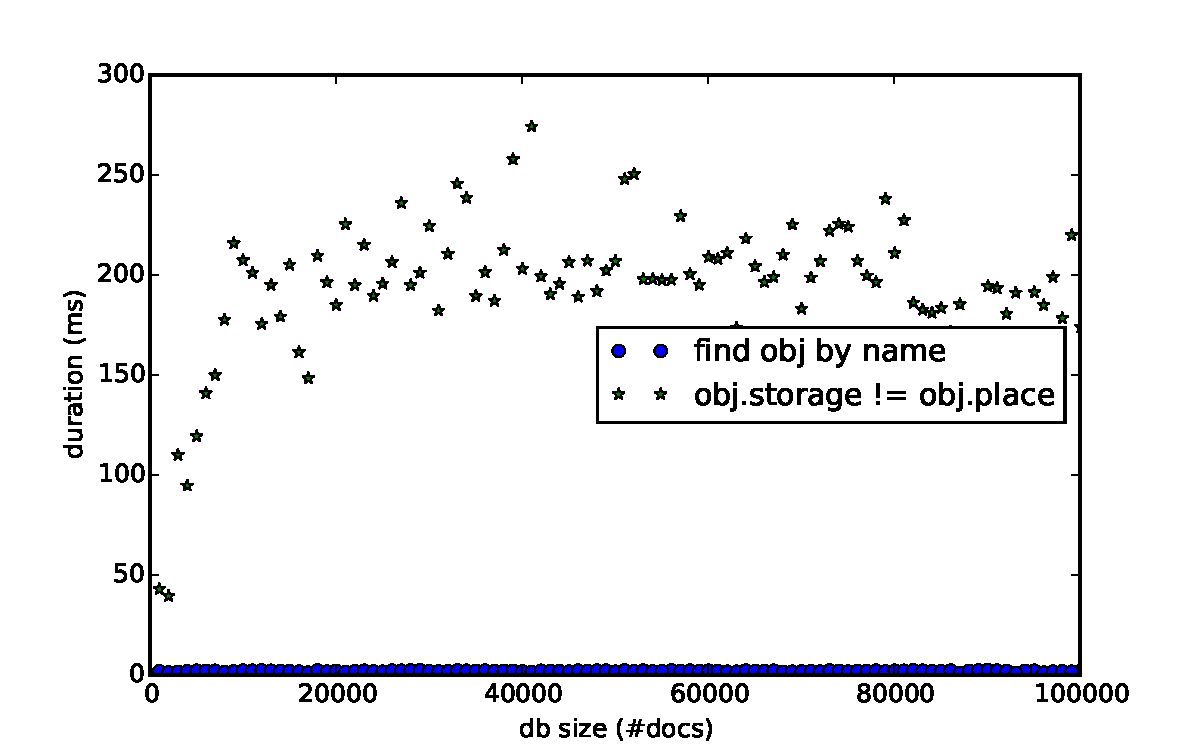
\includegraphics[width=\textwidth]{../thesis/plots/query-durations-index}\\
    \\\vspace{-0.05cm}
    (b) Queries
    \\\vspace{-0.1cm}
    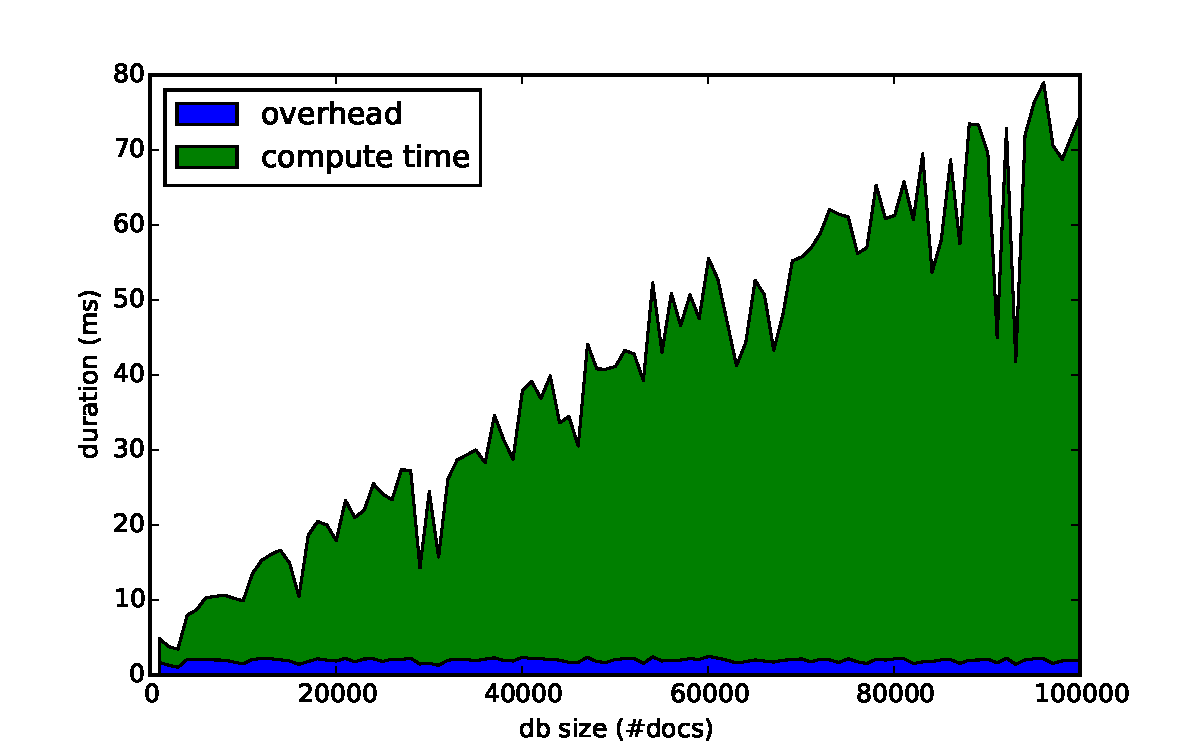
\includegraphics[width=\textwidth]{../thesis/plots/computable-durations-index}\\
    \\\vspace{-0.05cm}
    (d) Computables
    \end{column}
  \end{columns}
\end{frame}

\begin{frame}
  \frametitle{Evaluation: Benchmarks RCLL}
  \centering
  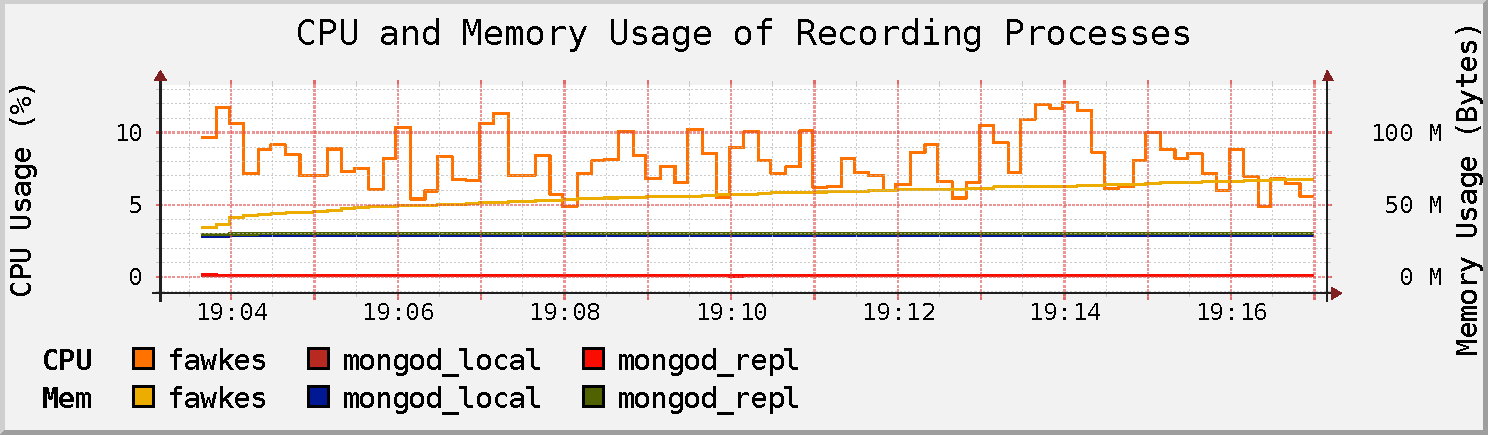
\includegraphics[width=0.8\textwidth]{../thesis/plots/rcll-local/cpu-mem}\\
  \vspace{0.1cm}
  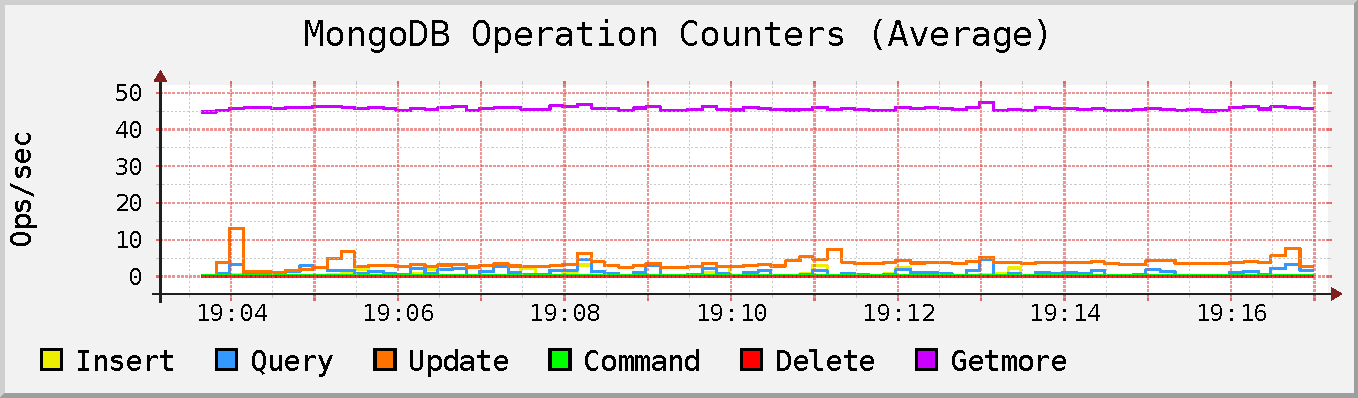
\includegraphics[width=0.8\textwidth]{../thesis/plots/rcll-local/operations}\\
  \vspace{0.1cm}
  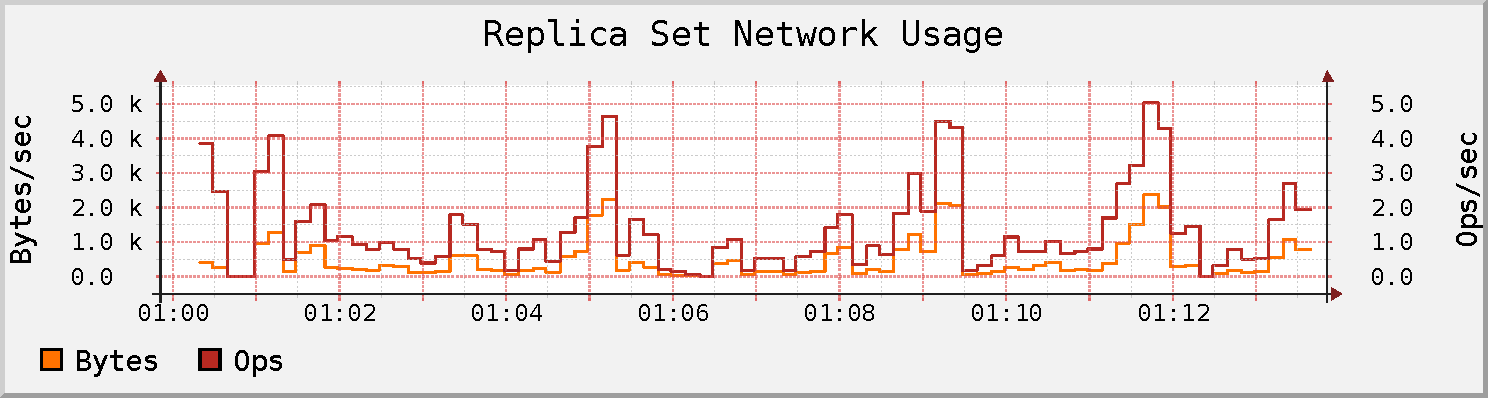
\includegraphics[width=0.8\textwidth]{../thesis/plots/rsnetwork}
\end{frame}

\begin{frame}
  \frametitle{Evaluation: Benchmarks Blocks World}
  \centering
  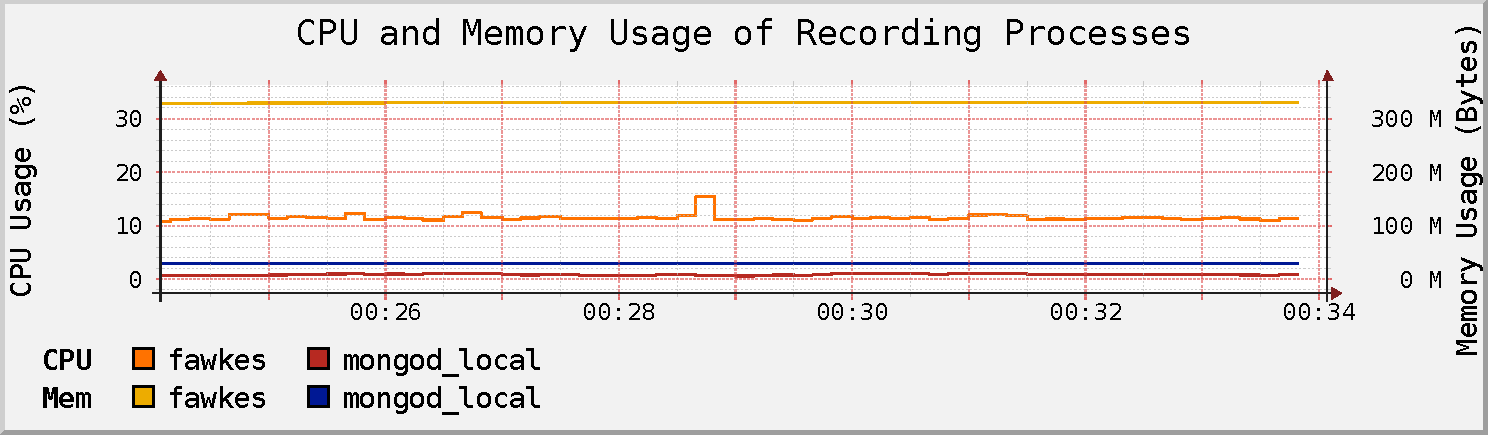
\includegraphics[width=0.8\textwidth]{../thesis/plots/blocksworld/cpu-mem}\\
  \vspace{0.1cm}
  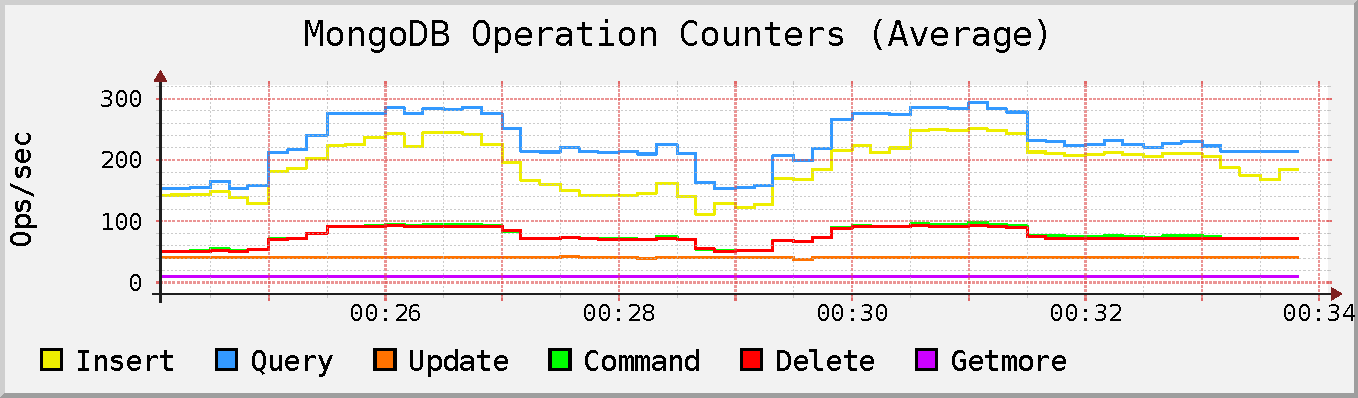
\includegraphics[width=0.8\textwidth]{../thesis/plots/blocksworld/operations}
\end{frame}

\begin{frame}
  \frametitle{Fawkes}
  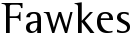
\includegraphics[width=0.25\textwidth]{../thesis/img/fawkes}  
  \bigskip
  \begin{itemize}
    \item Robot Software Framework % used in application domains
    \item Component-based software design % RM one of those components
    \item Hybrid blackboard communication infrastructure\\ with specific interfaces/messages % but no generic memory
      \skip
    \item[$\Rightarrow$] Robot Memory available as Fawkes plugin
  \end{itemize}
\end{frame}

\setcounter{framenumber}{\value{finalframe}}

\end{document}
